\documentclass[a4paper]{article}
%% Language and font encodings
\usepackage[english]{babel}
\usepackage[utf8x]{inputenc}
\usepackage[T1]{fontenc}
\usepackage{float}
%% Sets page size and margins
\usepackage[a4paper,top=3cm,bottom=2cm,left=3cm,right=3cm,marginparwidth=1.75cm]{geometry}

%% Useful packages
\usepackage{tensor}
\usepackage{tikz}
\usepackage{fancyhdr}
\pagestyle{fancy}
\usepackage{amsmath}
\usepackage{mathtools}
\usepackage{amstext}
\usepackage{amsthm}
\usepackage{enumitem}
\usepackage{eqnarray}
\usepackage{float}
\usepackage{esint}
\usepackage{wrapfig}
\usepackage{gensymb}
\usepackage{lipsum}
\usepackage{amssymb}
\usepackage{array}
\usepackage{tikz}
\usepackage[colorlinks=true, allcolors=blue]{hyperref}
\usepackage{graphicx}
\usepackage{amsmath}
\usepackage{amssymb}

\usepackage{graphicx}
\usepackage{mathtools}
\usepackage[caption=false]{subfig}
\DeclareMathOperator{\Sym}{Sym}
\DeclareMathOperator{\Auto}{Aut}
\DeclareMathOperator{\lcm}{lcm}
\DeclareMathOperator{\Tr}{Tr}
\DeclareMathOperator{\R}{Im}
\DeclareMathOperator{\Ker}{Ker}
\DeclareMathOperator{\sech}{sech}
\DeclareMathOperator{\diag}{diag}
\DeclareMathOperator{\sgn}{sgn}
\DeclareMathOperator{\Mod}{mod}
\DeclareMathOperator{\cl}{cl}
\newcommand{\iso}{\xrightarrow{
   \,\smash{\raisebox{-0.65ex}{\ensuremath{\scriptstyle\sim}}}\,}}
\newtheorem{post}{Postulate}[section]
\newtheorem{eg}{Example}[section]
\newtheorem{remarks}{Remarks}[section]
\newtheorem{notation}{Notation}[section]
\newtheorem{Note}{Note}[section]
\definecolor{darkblue}{RGB}{	0, 0, 139}
\newtheoremstyle{new}% <name>
{2pt}% <Space above>
{2pt}% <Space below>
{\color{darkblue}}% Body font
{}% <Indent amount>
{\bfseries\color{black}}% Theorem head font
{:}% <Punctuation after theorem head>
{.5em}% <Space after theorem headi>
{}% <Theorem head spec (can be left empty, meaning `normal')>
\theoremstyle{new}
\newtheorem{law}{Law}[section]
\newtheorem{defi}{Definition}[section]
\newtheorem{thm}{Theorem}[section]
\newtheorem{prop}{Proposition}[section]
\newtheorem{lemma}{Lemma}[section]
\newtheorem{cor}{Corollary}[section]


\title{\textbf{Part II REL Summary Notes}}
\author{Tai Yingzhe, Tommy (ytt26)}
\date{}
\setlength{\parindent}{0cm}
\begin{document}
\maketitle
\tableofcontents
\subsection*{Acknowledgements:}
Many thanks to my supervisor Mohammadreza Noormandipour, and the lecturer Anthony Challinor for their guidance. Some parts of this notes are heavily influenced by the Part II DAMTP course General Relativity (taught by Ulrich Sperhake).
\newpage
\section{Introduction}
\subsection{Units}
Traditionally, you may be familiar with the widespread usage of the SI units. Here, we adopt the natural units, where all the constants of nature are set as 1. This unifies physical dimensions and may highlight possible breakdowns of classical (Newtonian) theories. 
\begin{eg}[Speed of Light]
From now on, $c=1$. For speeds $v<<c$, we recover Newtonian mechanics. But this becomes problematic at $v$ close to 1, and we thus need Special Relativity.
\end{eg}
\begin{eg}[Gravitational Constant]
In addition, we further set $G=1$. In that case, 1 s $=3\times10^8$ m (from earlier) and 1 m $=1.3466\times10^{27}$ kg. In this case, the Solar mass is roughly 1.47 km (This is the Schwarzschild radius of the Sun, as we will see later). For $\frac{M}{R}<<\frac{c^2}{G}=1$, Newtonian gravity is accurate. But for $\frac{M}{R}\approx 1$, we will require General Relativity.
\end{eg}
\begin{eg}[Planck's Constant]
While we do not need $\hbar$ in this course, we further demonstrate the idea of natural units by setting $\hbar=1$. In that case, $\frac{\hbar}{mc}\approx R$ regime requires Quantum Mechanics, where $\frac{\hbar}{mc}=\frac{1}{m}$ is the Comptom wavelength.
\end{eg}
\subsection{Newtonian gravity}
\begin{defi}[Passive gravitational mass]
Passive gravitational mass $m_P$ is a measure of the strength of an object's interaction with a gravitational field.
\end{defi}
\begin{defi}[Poisson's equation/Gauss' Law for gravity]
The mass density of a gravitational source determines the divergence of gravitational field $\mathbf{g}$, or the Laplacian of the gravitational potential $\Phi$.
\begin{equation}4\pi G\rho=\boldsymbol{\nabla}\cdot\mathbf{g}=\nabla^2\Phi\label{Poisson}
\end{equation}
\end{defi}
\begin{defi}[Active gravitational mass]
Active gravitational mass $m_A$ is a measure of the strength of an object's gravitational flux (equal to the surface integral of gravitational field over an enclosing surface).
\end{defi}
\begin{prop}
The ratio of passive to active gravitational mass is the same for all particles.
\end{prop}
\begin{proof}
For a point particle at position $\mathbf{y}(t)$ at time $t$ is $\rho(\mathbf{x},t)=m_A\delta^{(3)}(\mathbf{x}-\mathbf{y}(t))$. The corresponding solution to Eqn.~\ref{Poisson} would be
$$\nabla^2\Phi=4\pi G\rho\implies\Phi(\mathbf{x},t)=-\frac{Gm_A}{|\mathbf{x}-\mathbf{y}(t)|}$$
The force on a test particle of passive mass $m_{P,1}$ at position $\mathbf{x_1}$ at time $t$ due to a particle of active mass $m_{A,2}$ at position $\mathbf{x_2}$ at the same time $t$ is
$$\mathbf{f_{2,1}}=-Gm_{P,1}m_{A,2}\frac{\mathbf{x_1}-\mathbf{x_2}}{|\mathbf{x_1}-\mathbf{x_2}|^3}$$
Similarly, $\mathbf{f_{1,2}}=-Gm_{P,2}m_{A,1}\frac{\mathbf{x_2}-\mathbf{x_1}}{|\mathbf{x_1}-\mathbf{x_2}|^3}$. The conservation of momentum gives $\mathbf{f_{2,1}}=-\mathbf{f_{1,2}}$, hence we have $\frac{m_{P,1}}{m_{P,2}}=\frac{m_{A,1}}{m_{A,2}}$.
\end{proof}
More generally, we have:
\begin{prop}
For mutual collinear forces, the magnitude of the passive source is equal to that of the active source.
\end{prop}
\begin{proof}
Follow from Newton's Third Law, together with the relevant force law.
\end{proof}
\begin{defi}[Inertial mass]
Inertial mass is the inertial resistance to acceleration of the body when responding to a force.
\end{defi}
\begin{prop}
Inertial mass is also the same as the active and passive mass.
\end{prop}
\newpage
\begin{remarks}\leavevmode
\begin{enumerate}
\item The equality of gravitational mass (passive source which determines the gravitational force on the particle) and inertial mass has been experimentally verified to one part in $10^{13}$. The many experiments that verified this, led to the equivalence principles.
\item Proposition 1.2 is true for both masses and electric charges, but not true for Proposition 1.3 since there is no concept of inertial charge.
\end{enumerate}
\end{remarks}
\begin{prop}[Weak Equivalence Principle (WEP)]
Freely falling bodies with negligible gravitational self-interaction follow the same path if they have the same initial velocity and position, independent of composition.
\end{prop}
\begin{defi}[Local Inertial Frame]
Local inertial frame is defined by a freely falling observer in the same way as an inertial frame is defined in Minkowski spacetime. Local means that the frame is much smaller than the length scale of gravitational field variations. 
\end{defi}
\begin{remarks}
For length scales large enough to observe gravitational field variations, we will experience tidal effects, which are physical manifestation of the gravitational field.
\end{remarks}
Einstein promoted the Weak Equivalence Principle.
\begin{prop}[Einstein Equivalence Principle]
In a local inertial frame, the results of all non-gravitational experiments are indistinguishable from those of the same experiment performed in an inertial frame in Minkowski spacetime.
\end{prop}
\begin{prop}[Strong Equivalence Principle (SEP)]
In an arbitrary gravitational field, all the laws of physics (not just the dynamics of free-falling particles) in a free-falling, non-rotating laboratory occupying a
sufficiently small region of spacetime look locally like
special relativity (with no gravity).
\end{prop}
\begin{remarks}
In particular, the SEP implies that a constant gravitational field is unobservable – observations in a reference frame at rest in such a field would be indistinguishable from those in a uniformly-accelerating reference frame in the absence of gravity.
\end{remarks}
\begin{defi}[General Relativity]
General relativity abandons the idea of gravity as a force defined on the fixed spacetime of special relativity, replacing it with a geometric theory in which the geometry of spacetime determines the trajectories of free-falling particles, the geometry itself being curved by the presence of matter.
\end{defi}
\begin{remarks}\leavevmode
\begin{enumerate}
\item The SEP implies the WEP, but not the other way round.
\item In the SEP, we require the test body to be small, so that tidal effects are negligible. 
\item The SEP is related to the equality of active and passive mass. 
\item The SEP implies that Newton’s gravitational constant G is the same everywhere in the universe, and suggests that gravity is entirely of geometrical nature. Otherwise, the gravitational binding energy of an extended object would depend on its position.
\item If the response of a body’s motion to gravitational forces is independent of the properties of the body, it suggests that the gravitational force is not a feature of the body but exclusively of the spacetime in which it moves. To be more precise, gravity is a feature of the spacetime’s geometry.
\end{enumerate}
\end{remarks}
\newpage
\subsection{Gravitational waves}
In the regime $|\Phi|<<c^2$, gravitational fields are weak and Newtonian gravity holds. But, this is not a good approximation. One experimental evidence that suggests Newtonian gravity is a poor model for gravity, is gravitational waves.
\begin{defi}[Gravitational Waves]
Gravitational waves are wavelike disturbances in the geometry of spacetime, which can be detected by looking for their characteristic quadrupole distortion (i.e., a shortening in one direction and stretching in an orthogonal direction) of the two arms of a laser interferometer.\\[5pt]
Gravitational waves propagate at the speed of light and are a natural prediction of general relativity; they do not arise in Newtonian gravity where the potential responds instantly to distant rearrangements of mass.
\end{defi}
\begin{eg}
The first LIGO signal was generated by a truly extreme astrophysical source: two merging black holes each with a mass around 30 times that of the Sun at a distance from us of around 2 Gly.\\[5pt]
As the black holes orbited their common centre of mass, the system radiated gravitational waves causing the black holes to spiral inwards and increase their speed until they merged to form a single black hole.\\[5pt]
Such sources probe the strong-field regime of general relativity during the merger phase and involve highly relativistic speeds. At its peak, the source was losing energy to gravitational waves at a rate of $3.6\times10^{49}$ W, which is equivalent to 200 times the rest mass energy of the Sun per second!
\end{eg}
\begin{remarks}
The Nobel Prize in Physics 2017 was divided, one half awarded to Rainer Weiss, the other half jointly to Barry C. Barish and Kip S. Thorne `for decisive contributions to the LIGO detector and the observation of gravitational waves'.
\end{remarks}
\newpage
\section{Special relativity recap}
We recap the concepts from IA Special Relativity.
\subsection{Galilean transformations}
\begin{defi}[Inertial frames]
  Inertial frames are frames of references in which the frames themselves are not accelerating. Newton's Laws only hold in inertial frames.
\end{defi}
\begin{defi}[Galilean transformations]
  Two inertial frames are related by
  \begin{itemize}
  \item Translations of space:
    \[
      \mathbf{r}' = \mathbf{r} - \mathbf{r}_0
    \]
  \item Translations of time:
    \[
      t' = t - t_0
    \]
  \item Rotation (and reflection):
    \[
      \mathbf{r}' = R\mathbf{r}
    \]
    with $R\in O(3)$.
\end{itemize}
\end{defi}
They are simply symmetries of space itself.
\begin{defi}[Galilean boost]
  A Galilean boost is a change in frame of reference by
  \begin{align*}
    \mathbf{r}' &= \mathbf{r} - \mathbf{v}t\\
    t' &= t
  \end{align*}
  for a fixed, constant $\mathbf{v}$, i.e. uniform motion.
\end{defi}
All these transformations together generate the Galilean group, which describes the symmetry of Newtonian equations of motion.
\begin{law}[Galilean relativity]
  The principle of relativity asserts that the laws of physics are the same in all inertial frames.
\end{law}
\begin{remarks}
The equations of Newtonian physics must have Galilean invariance. Since the laws of physics are the same regardless of your velocity, velocity must be a relative concept, and there is no such thing as an ``absolute velocity'' that all inertial frames agree on. However, all inertial frames must agree on whether you are accelerating or not (even though they need not agree on the direction of acceleration since you can rotate your frame). So acceleration is an absolute concept.
\end{remarks}
\begin{remarks}[Special Relativity]
In special relativity, we abandon the notion of absolute time. It is replaced by a new postulate: The speed of light $c$ is the same in all inertial frames.
\end{remarks}
\subsection{The Lorentz transformation}
\begin{prop}
  Consider inertial frames $S$ and $S'$ whose origins coincide at $t = t' = 0$, and that $S'$ moves with velocity $v$ relative to $S$, then the Lorentz transformation must be of the form
  $$x'=\gamma(x-vt)$$
  for some factor $\gamma$.
\end{prop}
\begin{proof}
 For now, neglect the $y$ and $z$ directions, and consider the relationship between $(x, t)$ and $(x', t')$. The general form is
$$x' = f(x, t),\quad t' = g(x, t)$$
for some functions $f$ and $g$. In any inertial frame, a free particle moves with constant velocity. So straight lines in $(x, t)$ must map into straight lines in $(x', t')$. Therefore the relationship must be linear. The line $x = vt$ must map into $x'= 0$, hence the result. We can use symmetry arguments to show that $\gamma$ should take the same value for velocities $v$ and $-v$).
\end{proof}
\begin{remarks}
Now reverse the roles of the frames. From the perspective $S'$, $S$ moves with velocity $-v$. A similar argument leads to $x=\gamma(x'+vt')$ for the same $\gamma$, which is only dependent on $|v|$.
\end{remarks}
\begin{prop}
  The factor $\gamma$ is called the Lorentz factor and it is called
  $$\gamma=\frac{1}{\sqrt{1-v^2/c^2}}$$
\end{prop}
\begin{proof}
Now consider a light ray (or photon) passing through the origin $x = x' = 0$ at $t = t' = 0$. Its trajectory in $S$ is
$x = ct$. We want a $\gamma$ such that the trajectory in $S'$ is $x' = ct'$ as well, so that the speed of light is the same in each frame. Substitute these into the Lorentz transformation equation and its inverse transform, and multiply them together, and finally divide by $tt'$ to obtain
$$ct'ct=\gamma(ct-vt)\gamma(ct'+vt')\implies c^2 = \gamma^2(c^2 - v^2)\implies \gamma = \sqrt{\frac{c^2}{c^2 - v^2}} = \frac{1}{\sqrt{1 - (v/c)^2}}$$
\end{proof}
\begin{prop}
  The Lorentz transformation between times in two inertial frames is
  $$t'=\gamma(t-vx/c^2)$$
\end{prop}
\begin{proof}
Eliminate $x$ between the Lorentz transformation equation and its inverse,
$$x = \gamma(\gamma(x - vt) + vt')\implies
t' = \gamma t - (1 - \gamma^{-2})\frac{\gamma x}{v} = \gamma\left(t - \frac{v}{c^2}x\right)$$
\end{proof}
\begin{defi}[Standard Lorentz boosts]
\begin{equation}
x'=\gamma(x-vt),\quad t'=\gamma(t-vx/c^2)\label{boost}
\end{equation}
\end{defi}
\begin{remarks}
Directions perpendicular to the relative motion of the frames are unaffected.
\end{remarks}
\begin{remarks}[Generic Lorentz boosts]
More generally, the relation between two Cartesian inertial frames $S$ and $S'$ can differ from that for the standard configuration since
\begin{enumerate}
    \item the spacetime origins may not coincide, i.e. the event at $ct=x=y=z=0$ may not be at $ct'=x'=y'=z'=0$
    \item the relative velocity of the two frames may be in an arbitrary direction in $S$, rather than along the $x$-axis
    \item the spatial axes in $S$ and $S'$ may not be aligned
\end{enumerate}
The generic procedure is
\begin{enumerate}
    \item align the spacetime origins by appropriate temporal and spatial displacements
    \item apply a purely spatial rotation in frame $S$ to align the new $x$-axis with the relative velocity of the two frames
    \item apply a standard Lorentz transform
    \item apply a spatial rotation in the transformed coordinates to align the axes with those of $S'$.
\end{enumerate}
\end{remarks}
\newpage
\subsection{Spacetime diagrams}
It is often helpful to plot out what is happening on a diagram. We plot them on a graph, where the position $x$ is on the horizontal axis and the time $ct$ is on the vertical axis. We use $ct$ instead of $t$ so that the dimensions make sense.
\begin{defi}[Spacetime]
  The union of space and time in special relativity is called Minkowski spacetime. Each point $P$ represents an event, labelled by coordinates $(ct, x)$. 
\end{defi}
\begin{defi}[World lines]
  A particle traces out a world line in spacetime, which is straight if the particle moves uniformly. Light rays moving in the $x$ direction have world lines inclined at $45^\circ$.
\end{defi}
\begin{remarks}
We can also draw the axes of $S'$, moving in the $x$ direction at velocity $v$ relative to $S$. The $ct'$ axis corresponds to $x' = 0$, i.e.\ $x = vt$. The $x'$ axis corresponds to $t' = 0$, i.e.\ $t = vx/c^2$. Note that the $x'$ and $ct'$ axes are not orthogonal, but are symmetrical about the diagonal (dashed line). So they agree on where the world line of a light ray should lie on.
\end{remarks}
\begin{remarks}
For a massive particle passing through an event A, the particle's worldline must be inside the light cone through A and each infinitesimal step must lie within the light cone at each point. For a photon, the worldline will be tangent to the light cone.
\end{remarks}
\begin{defi}[Simultaneous events]
  We say two events $P_1$ and $P_2$ are simultaneous in the frame $S$ if $t_1 = t_2$.
\end{defi}
\begin{remarks}[Causality]
Although different observers may disagree on the temporal order of events, the consistent ordering of cause and effect can still be ensured since information can only travel at, at most the speed of light. We can draw a light cone that denotes the regions in which things can be influenced by an event $P$. These are the regions of space-time light (or any other particle) can possibly travel to. $P$ can only influence events within its future light cone, and be influenced by events within its past light cone.
\end{remarks}
\begin{defi}[Invariant interval]
  The spacetime interval between $P$ and $Q$ is defined as
$$\Delta s^2 = c^2 \Delta t^2 - \Delta x^2$$
  Note that this quantity $\Delta s^2$ can be both positive or negative.
\end{defi}
\begin{prop}
  All inertial observers agree on the value of $\Delta s^2$.
\end{prop}
\begin{proof} From Eqn.~\ref{boost},
$$c^2 \Delta t'^2 - \Delta x'^2 = c^2 \gamma^2 \left(\Delta t - \frac{v}{c^2}\Delta x\right)^2 - \gamma^2 (\Delta x - v\Delta t)^2= \gamma^2 \left(1 - \frac{v^2}{c^2}\right)(c^2 \Delta t^2 - \Delta x^2)= c^2\Delta t^2 - \Delta x^2$$
Here, $\Delta x$ can be extended to $\Delta\vec{x}\in\mathbb{R}^3$.
\end{proof}
\begin{remarks}
This allow us to calibrate the spacetime axes with respect to the invariant $\Delta s^2$.
\end{remarks}
\begin{defi}[Line element]
  The line element is
  \begin{equation}
d s^2 = c^2 d t^2 - d x^2 - d y^2 - d z^2\label{ds2}
\end{equation}
\end{defi}

\begin{defi}[Timelike, spacelike and lightlike separation]\leavevmode
\begin{itemize}
  \item Events with $\Delta s^2 > 0$ are timelike separated. It is possible to find inertial frames in which the two events occur in the same position, and are purely separated by time. Timelike-separated events lie within each other's light cones and can influence one another.
  \item Events with $\Delta s^2 < 0$ are spacelike separated. It is possible to find inertial frame in which the two events occur in the same time, and are purely separated by space. Spacelike-separated events lie out of each other's light cones and cannot influence one another.
  \item Events with $\Delta s^2 = 0$ are lightlike or null separated. In all inertial frames, the events lie on the boundary of each other's light cones. e.g.\ different points in the trajectory of a photon are lightlike separated, hence the name.
\end{itemize}
\end{defi}
\begin{defi}[4-vector]
  A 4-vector is a four-component vector to describe an object's property in spacetime, in any inertial frame.
\end{defi}
\begin{defi}[4-Position]
The coordinates of an event $P$ in frame $S$ can be written as a 4-vector $X$. We write $X=(ct,\vec{x})^T$ where $\vec{x}$ is the 3-position, i.e. $\vec{x}\in\mathbb{R}^3$.
\end{defi}
\begin{prop}
The invariant interval between the origin and $P$ can be written as an inner product. The inner product of any two 4-vectors on the Minkowski metric $\eta$ is
$$X\cdot X = X^T\eta X = c^2t^2 - x^2 - y^2 - z^2,\quad\eta =
  \begin{pmatrix}
    1 & 0 & 0 & 0\\
    0 & -1 & 0 & 0\\
    0 & 0 & -1 & 0\\
    0 & 0 & 0 & -1
  \end{pmatrix}$$
4-vectors with $X\cdot X > 0$ are called timelike, and those $X \cdot X < 0$ are spacelike. If $X\cdot X = 0$, it is lightlike or null.
\end{prop}
\begin{defi}[Lorentz transformation]
A Lorentz transformation is a linear transformation of the coordinates from one frame $S$ to another $S'$, represented by a $4\times 4$ tensor: $X' = \Lambda X$. Lorentz transformations can be defined as those that leave the inner product invariant, (i.e. $\forall X$, $X'\cdot X' = X\cdot X)$ which implies the matrix equation
$$\Lambda^T\eta \Lambda = \eta$$
These also preserve $X\cdot Y$ if $X$ and $Y$ are both 4-vectors.
\end{defi}
\begin{prop}
Two classes of solution to this equation are:
$$\Lambda =
  \begin{pmatrix}
    1 & 0 & 0 & 0\\
    0\\
    0 & & R\\
    0
  \end{pmatrix},\quad \begin{pmatrix}
    \gamma & -\gamma \beta & 0 & 0\\
    -\gamma\beta & \gamma & 0 & 0\\
    0 & 0 & 1 & 0\\
    0 & 0 & 0 & 1
  \end{pmatrix}$$
The former rotates space only and leaves time intact, where $R$ is a $3\times 3$ orthogonal matrix. For the latter, $\beta = \frac{v}{c}$, and $\gamma = 1/\sqrt{1 - \beta^2}$. Here we leave the $y$ and $z$ coordinates intact, and apply a Lorentz boost along the $x$ direction.
\end{prop}
\begin{remarks}
The set of all matrices satisfying $\Lambda^T\eta\Lambda=\eta$ form the Lorentz group $O(1, 3)$. It is generated by rotations and boosts, as defined above, which includes the absurd spatial reflections and time reversal. The subgroup with $\det \Lambda = +1$ is the proper Lorentz group $SO(1, 3)$.\\[5pt]
The subgroup that preserves spatial orientation and the direction of time is the restricted Lorentz group $SO^+(1, 3)$. Note that this is different from $SO(1, 3)$, since if you do both spatial reflection and time reversal, the determinant of the matrix is still positive. We want to eliminate those as well!
\end{remarks}
\begin{defi}[Rapidity]
  The rapidity of a Lorentz boot is $\phi$ such that
\begin{equation}
    \beta = \tanh \phi,\quad \gamma = \cosh\phi,\quad \gamma\beta=\sinh \phi\label{rapidity}
\end{equation}
\end{defi}
\begin{remarks}
Focus on the upper left $2\times 2$ matrix of Lorentz boosts in the $x$ direction. Write
$$\Lambda[\beta] =
  \begin{pmatrix}
    \gamma & -\gamma\beta\\
    -\gamma\beta & \gamma
  \end{pmatrix}
  ,\quad
  \gamma = \frac{1}{\sqrt{1 - \beta^2}}$$
Combining two boosts in the $x$ direction, we have
$$\Lambda[\beta_1]\Lambda[\beta_2] =
  \begin{pmatrix}
    \gamma_1 & -\gamma_1\beta_1\\
    -\gamma_1\beta_1 & \gamma_1
  \end{pmatrix}
  \begin{pmatrix}
    \gamma_2 & -\gamma_2\beta_2\\
    -\gamma_2\beta_2 & \gamma_2
  \end{pmatrix}
  = \Lambda\left[\frac{\beta_1 + \beta_2}{1 + \beta_1\beta_2}\right]$$
This is consistent with the idea of spatial rotations and thus add like rotation angles.
$$\Lambda[\beta] =
  \begin{pmatrix}
    \cosh \phi & -\sinh \phi\\
    -\sinh \phi & \cosh \phi
  \end{pmatrix}
  = \Lambda(\phi),\quad\Lambda(\phi_1)\Lambda(\phi_2) = \Lambda(\phi_1 + \phi_2)$$
Lorentz boots are simply hyperbolic rotations in spacetime!
\end{remarks}
\subsection{Relativistic kinematics}
\begin{defi}[Proper time]
  The proper time $\tau$ is defined such that
$$\Delta \tau = \frac{\Delta s}{c}$$
  $\tau$ is the time experienced by the particle, i.e.\ the time in the particles rest frame, the instantaneous rest frame (IRF) of the particle.
\end{defi}
\begin{remarks}
The world line of a massive particle can be parametrized using the proper time by $t(\tau)$ and $\mathbf{x}(\tau)$. Infinitesimal changes are related by
\begin{equation}
d \tau = \frac{d s}{c} = \frac{1}{c}\sqrt{c^2dt^2 - |d \vec{x}|^2} = \sqrt{1 - \frac{|\vec{u}|^2}{c^2}}\;d t,\quad\frac{d t}{d \tau} = \gamma_u= \frac{1}{\sqrt{1 - \frac{|\vec{u}|^2}{c^2}}}\label{propertime}
\end{equation}
The total time experienced by the particle along a segment of its world line is
$$T = \int \;d \tau = \int\frac{1}{\gamma_u}\;d t$$
\end{remarks}
\begin{eg}[Doppler Effect]
Consider an observer $\mathcal{E}$ who moves at speed $v$ along the $x$-axis of an inertial frame $S$ in which an observer $\mathcal{O}$ is at rest at position $x_0$. Let successive wavecrests be emitted by $\mathcal{E}$ at events A and B, which are separated by proper time $\Delta\tau_{AB}$, i.e. this is the proper period of the source. The relation between $\Delta\tau_{AB}$ and the time between the emission events in $S$ is
$$\Delta\tau_{AB}=\sqrt{1-\frac{v^2}{c^2}}\Delta t_e$$
The wavecrests are received by $\mathcal{O}$ at the events C and D, which are separated by time $\Delta t_o$ in $S$; since $\mathcal{O}$ is at rest in $S$, the proper time between $C$ and $D$ is $\Delta\tau_{CD}=\Delta t_o$. In time $\Delta t_e$, the source $\mathcal{E}$ moves a distance $\Delta x_e=v\Delta t_e$ along the $x$-axis in $S$, and the second wavecrest has to travel $\Delta x_e$ further than the first to be received by $\mathcal{O}$ at $x_o$. Then,
$$\Delta t_o=\bigg(1+\frac{v}{c}\bigg)\Delta t_e$$
so that the ratio of proper times is
\begin{equation}
\frac{\Delta\tau_{AB}}{\Delta\tau_{CD}}=\frac{(1-\beta^2)^{1/2}\Delta t_e}{(1+\beta)\Delta t_e}=\sqrt{\frac{1-\beta}{1+\beta}}\label{Doppler}
\end{equation}
This ratio is also the ratio of the received frequency, as measured by $\mathcal{O}$, to the proper frequency (i.e., the frequency in the rest-frame of the source $\mathcal{E}$).
\end{eg}
\begin{defi}[4-velocity]
Its 4-velocity is defined as
\begin{equation}
U = \frac{d X}{d \tau} =
    \begin{pmatrix}
      c\frac{d t}{d \tau}\\
      \frac{d \vec{x}}{d \tau}
    \end{pmatrix}
    = \frac{d t}{d \tau}
    \begin{pmatrix}
      c\\
      \vec{u}
    \end{pmatrix} = \gamma_u
    \begin{pmatrix}
      c\\
      \vec{u}
    \end{pmatrix},\quad\vec{u} = \frac{d \vec{x}}{d t}\label{4-vel}
\end{equation}
\end{defi}
\begin{remarks}
$U$ is a 4-vector because $X$ is a 4-vector and $\tau$ is a Lorentz invariant. For any 4-vector $U$, the inner product $U\cdot U = U' \cdot U'$ is Lorentz invariant, i.e.\ the same in all inertial frames. In the rest frame of the particle, $U = (c, 0)$. So $U\cdot U = c^2$. In any other frame, $Y = \gamma_u(c, \vec{u})$. So
$$ Y\cdot Y = \gamma_u^2 (c^2 - |\vec{u}|^2) = c^2$$
\end{remarks}
\begin{prop}
A particle moves with constant velocity $u\mathbf{\hat{x}}$ in frame $S$. In a frame $S'$ which moves with velocity $v\mathbf{\hat{x}}$ relative to $S$, the velocity is
$$u'=\frac{u-v}{1-uv/c^2}$$
\end{prop}
\begin{proof}
The world line of the particle in $S'$ is $x'=u't'$. In $S$, using the inverse Lorentz transformation,
$$u = \frac{x}{t} = \frac{\gamma(x' + vt')}{\gamma(t' + (v/c^2) x')} = \frac{u't' + vt'}{t' + (v/c^2)u't'} = \frac{u' + v}{1 + u'v/c^2}$$
This is the formula for the relativistic composition of of velocities. The inverse transformation is found by swapping $u$ and $u'$, and swapping the sign of $v$.
\end{proof}
\begin{remarks}\leavevmode
\begin{enumerate}
\item If instead, the particle moves with constant velocity $u_x\mathbf{\hat{x}}+u_y\mathbf{\hat{y}}$ in frame $S$, then the transformation for the velocities perpendicular to the boost is
$$u'_y=\frac{u_y}{\gamma_v(1-u_xv/c^2)}$$
\item It will be more natural to perform collinear velocity addition by adding rapidities. Consider three inertial frames, where $S_0$ and $S_1$ are related by a standard boost along the $x$-direction with speed $v$, $S_1$ and $S_2$ are related by a standard boost along the $x'$-direction with speed $u'$. Let $\tanh\psi_v=v/c$, $\tanh\psi_{u'}=u'/c$, then it follows that $S_2$ is related to $S_0$ by a Lorentz boost in the $x$-direction with speed 
$$u=c\tanh(\psi_v+\psi_{u'})=\frac{c\tanh\psi_v+\tanh\psi_{u'}}{1+\tanh\psi_v\tanh\psi_{u'}}=\frac{u'+v}{1+u'v/c^2}$$
\end{enumerate}
\end{remarks}
\begin{prop}
Consider a generic motion - not parallel to the Lorentz boost. In frame $S$, consider a particle moving with speed $u$ at an angle $\theta$ to the $x$ axis in the $xy$ plane. In $S'$, the composition of parallel velocities will give
\begin{equation}
u'\cos \theta' = \frac{u\cos \theta - v}{1 - \frac{uv}{c^2}\cos \theta}\text{ while }
  \tan \theta' = \frac{u\sin \theta}{\gamma_v(u\cos \theta - v)}\label{velboost}
\end{equation}
which describes aberration, a change in the direction of motion of a particle due to the motion of the observer. 
\end{prop}
\begin{proof}
The 4-velocity (Eqn.~\ref{4-vel}) is
$$U =
  \begin{pmatrix}
    \gamma_u c\\
    \gamma_u u\cos \theta\\
    \gamma_u u\sin \theta\\
    0
  \end{pmatrix}\implies  U' = \begin{pmatrix}
    \gamma_{u'} c\\
    \gamma_{u'} u'\cos \theta'\\
    \gamma_{u'} u'\sin \theta'\\
    0
  \end{pmatrix}
  =
  \begin{pmatrix}
    \gamma_v & -\gamma_v v/c & 0 & 0\\
    -\gamma_{v} v/c & \gamma_v & 0 & 0\\
    0 & 0 & 1 & 0\\
    0 & 0 & 0 & 1
  \end{pmatrix}
  \begin{pmatrix}
    \gamma_u c\\
    \gamma_u u\cos \theta\\
    \gamma_u u\sin \theta\\
    0
  \end{pmatrix}$$
where we have frames $S$ and $S'$ to be in standard configuration (i.e.\ origin coincide at $t = 0$, $S'$ moving in $x$ direction with velocity $v$ relative to $S$). The results can be obtained by dividing the respective rows.
\end{proof}
\begin{remarks}\leavevmode
\begin{enumerate}
\item If $u=c$, we have the light aberration formula, obtained from Eqn.~\ref{velboost}:
\begin{equation}
\cos\theta'=\frac{\cos\theta-\beta}{1-\beta \cos\theta},\quad\tan\theta'=\frac{\sin\theta}{\gamma_u(\cos\theta-\beta)}\label{aberration}
\end{equation}
\item Suppose the radiation distribution is isotropic in the moving frame $S'$, i.e. $P(\theta',\phi')=\frac{1}{4\pi}$. Integrate over $\phi$:
$$P(\theta')d\theta'=\int_0^{2\pi}P(\theta',\phi')\sin\theta'd\theta'd\phi'=\frac{1}{2}\sin\theta'd\theta'$$
The number of photons emitted in either frame is the same, so
$$P(\theta)d\theta=P(\theta')d\theta'\implies P(\theta)=-\frac{1}{2}\frac{d\cos\theta'}{d\cos\theta}\frac{d\cos\theta}{d\theta}=\frac{\sin\theta}{2\gamma^2(1-\beta\cos\theta)^2}$$
where we differentiate $\cos\theta'=\frac{\cos\theta-\beta}{1-\beta\cos\theta}$ (Eqn.~\ref{aberration}), i.e. the photons are strongly ‘beamed’ in the x-direction due to aberration.
\end{enumerate}
\end{remarks}
\begin{defi}[4-acceleration]
The 4-acceleration is defined as
$$ A = \frac{d U}{d \tau}$$
where
\begin{equation}
U = \gamma_u
  \begin{pmatrix}
    c\\
    \vec{u}
  \end{pmatrix}
\implies A = \gamma_u \frac{d U}{d t} = \gamma_u
  \begin{pmatrix}
    \dot{\gamma}_u c\\
    \gamma_u \vec{a} + \dot{\gamma}_u \vec{u}.
  \end{pmatrix},\quad
\vec{a} = \frac{d \vec{u}}{d t},~\dot{\gamma}_u = \gamma_u^3 \frac{\vec{a}\cdot \vec{u}}{c^2}\label{4-acc}
\end{equation}
\end{defi}
\begin{prop}
$U\cdot A=0$ in all inertial frames.
\end{prop}
\begin{proof}
In the instantaneous rest frame of a particle, $\vec{u} = \vec{0}$ and $\gamma_u = 1$. So from Eqns.~\ref{4-vel} and \ref{4-acc}:
$$U =
  \begin{pmatrix}
    c\\
    \vec{0}
  \end{pmatrix}, \quad
  A =
  \begin{pmatrix}
    0\\
    \vec{a}
  \end{pmatrix}$$
Then $U\cdot A = 0$. Since the inner product between any two 4-vector is a Lorentz invariant quantity, we have $U\cdot A = 0$ in all frames.
\end{proof}
\begin{remarks}
Acceleration is not invariant in special relativity, but is however, an absolute quantity in that all observers agree whether a particle is accelerating or not.
\end{remarks}
\begin{cor}
For a Lorentz boost along the $x$-direction, we have
\begin{equation}
\vec{a'}=\begin{pmatrix}(\gamma_v(1-u_xv/c^2))^{-3}&0&0\\\frac{u_yv}{c^2\gamma_v^2(1-u_xv/c^2)^3}&(\gamma_v(1-u_xv/c^2))^{-2}&0\\\frac{u_zv}{c^2\gamma_v^2(1-u_xv/c^2)^3}&0&(\gamma_v(1-u_xv/c^2))^{-2}\\\end{pmatrix}\vec{a}\label{accboost}
\end{equation}
\end{cor}
\begin{proof}
The accelerations are obtained by taking differentials from the velocity transformations (Eqn.~\ref{velboost}):
$$du_x'=\frac{du_x}{\gamma_v^2(1-u_xv/c^2)^2},~ du_y'=\frac{du_y}{\gamma_v(1-u_xv/c^2)}+\frac{u_yvdu_x}{c^2\gamma_v(1-u_xv/c^2)^2},~ du_z'=\frac{du_z}{\gamma_v(1-u_xv/c^2)}+\frac{u_zvdu_x}{c^2\gamma_v(1-u_xv/c^2)^2}$$
Finally, note that $dt'=\gamma_v(1-u_xv/c^2)dt$.
\end{proof}
\begin{prop}[Rectilinear acceleration]
Consider a particle moving at a variable speed $u(\tau)$ along the $x$-axis in the inertial frame $S$, where $\tau$ is the particle’s proper time. Let the particle carry an accelerometer that reads $f(\tau)$ – this is the proper acceleration, the acceleration in the instantaneous rest frame of the particle at $\tau$. In terms of rapidity, we have
$$c\psi(\tau)=\int_0^\tau f(\tau')d\tau'$$
\end{prop}
\begin{proof}
In the instantaneous rest frame at $\tau$, $u'(\tau)=0$ and $\frac{du'}{dt'}=f(\tau)$. Transforming back to the frame $S$ (Eqn.~\ref{accboost}), we have
$$\frac{du}{dt}=\frac{\frac{du'(\tau)}{d\tau}}{\gamma_u^3(1-0)^3}=\bigg(1-\frac{u^2}{c^2}\bigg)^{3/2}f(\tau)\implies\frac{du}{d\tau}=\bigg(1-\frac{u^2}{c^2}\bigg)f(\tau)$$
Integrating, we have
$$\int\frac{du}{1-\frac{u^2}{c^2}}=\int f(\tau)d\tau\implies c\tanh^{-1}(u/c)=\int f(\tau)d\tau$$
In terms of rapidity $\psi(\tau)$, i.e.  $u(\tau)=c\tanh\psi(\tau)$ (Eqn.~\ref{rapidity}), we have
$$\bigg(1-\frac{u^2}{c^2}\bigg)f(\tau)=\frac{du}{d\tau}=c\sech^2\psi(\tau)\frac{d\psi(\tau)}{d\tau}\implies c\frac{d\psi}{d\tau}=f(\tau)\implies c\psi(\tau)=\int_0^\tau f(\tau')d\tau'$$
where $u(\tau=0)=0$. 
\end{proof}
\newpage
\begin{eg}
To parameterise the worldline of the particle in $S$, we can use Eqn.~\ref{rapidity}:
$$\frac{dt}{d\tau}=\gamma_u=\cosh\psi(\tau),\quad\frac{dx}{d\tau}=u\gamma_u=c\sinh\psi(\tau)$$
Integrating these equations gives the coordinates in $S$ of the wordline, $t(\tau)$ and $x(\tau)$. Consider now the simple case of uniform or constant proper acceleration, i.e. $f=\text{const}$. The rapidity rises linearly with $\tau$, i.e. $\psi(\tau)=f\tau/c$, and the worldline is
$$t=t_0+\frac{c}{f}\sinh\frac{f\tau}{c},\quad x-x_0=\frac{c^2}{f}\bigg[\cosh\frac{f\tau'}{c}\bigg]_0^\tau=\frac{c^2}{f}\bigg(\cosh\frac{f\tau}{c}-1\bigg)$$
where $t_0$ and $x_0$ are integration constants. Setting $ct_0=x_0=0$, we have a hyperbolic trajectory through the origin, as shown to the right, with an oblique asymptote in the future of $ct = c^2/f + x$. This means that there are regions of spacetime containing events that can never influence (i.e., communicate causally with) the accelerated particle (events to the left of the dotted line). The boundary of this region defines an event horizon of the accelerated observer.\\[5pt]
As an example, light emitted from an object at rest at $x = 0$ in $S$ will only reach the accelerated observer if it is emitted before $t = c/f$. Moreover, the accelerated observer sees the emitted light Doppler shifted to longer and longer wavelengths as the object approaches the event horizon and is observed as $\tau\rightarrow\infty$.
\end{eg}
\begin{center}
\begin{tikzpicture}
      \draw[->] (-1,0) -- (3,0) node[right] {$x$};
      \draw[->] (0,0) -- (0,4) node[left] {$ct$};
      \draw[domain=-0.1:3,smooth,variable=\x,black] plot ({\x},{\x+0.1});
      \draw[domain=1:3,smooth,variable=\x,blue] plot ({\x},{sqrt(\x^2-1)});
      \draw (0,0.1) node[left]{$c^2/f$};
      \draw (0,0) node[below]{0};
    \end{tikzpicture}
\end{center}
\newpage
\section{Differential geometry}
The spacetime of special relativity – Minkowski spacetime – is an example of what mathematicians call a manifold. In general relativity, spacetime is described by a more complicated manifold that responds dynamically to the distribution of mass and energy.
\subsection{Manifolds and coordinates}
\subsubsection{Manifolds and coordinate transformation}
\begin{defi}[Manifold]
An $n$-dimensional manifold $\mathcal{M}$ is a set of points with a bijective map to $\mathbb{R}^n$.
$$\phi:~\mathcal{M}\rightarrow U\subset\mathbb{R}^n,\quad p\in\mathcal{M}\mapsto x^\alpha\in U\subset\mathbb{R}^n,\quad\alpha\in[0,n-1]$$
where $U$ is an open subset of $\mathbb{R}^n$. $x^\alpha$ are the coordinates of point $p$ on $\mathcal{M}$.
\end{defi}
\begin{remarks}\leavevmode
\begin{enumerate}
\item Informally, an N-dimensional manifold is a set of objects that locally resembles N-dimensional Euclidean space $\mathbb{R}^N$.
\item It is not strictly required that we have one map $\phi$ that globally covers the entire manifold $\mathcal{M}$. It is, however, sufficient to partition $\mathcal{M}$ and map each part separately to $\mathbb{R}^n$. Everything we will develop also holds for such subdivisions of $\mathcal{M}$. 
\item The manifold is differentiable if these subdivisions join up smoothly so that we can define scalar fields on the manifold that are differentiable everywhere.
\item Operations (taking derivatives) and objects (curves, vectors etc) live on $\mathcal{M}$, not in the coordinate space $U$. But $\phi$ is one-to-one, so this distinction often blurred.
\item We can generally think of manifolds as surfaces embedded in some higher-dimensional Euclidean space, and we shall often do so, but it is important to appreciate that a given manifold exists independent of any embedding.
\item The coordinates are not unique: think of them as labels of points in the manifold that can change under a coordinate transformation (i.e., a change of map $\phi$) while the point itself does not.
\end{enumerate}
\end{remarks}
\begin{eg}\leavevmode
\begin{enumerate}
    \item The Euclidean plane $\mathbb{R}^2$ is a 2D manifold that can be covered globally with the usual Cartesian coordinates. However, we could instead use plane-polar coordinates, $(\rho, \phi)$ with $0\leq\rho<\infty$ and $0\leq\phi<2\pi$. Plane-polar coordinates are degenerate at $\rho= 0$ since $\phi$ is indeterminate there.
    \item The 2-sphere $\mathcal{S}^2$ is the set of points in $\mathbb{R}^3$ with $x^2+y^2+z^2 =1$. It is an example of a 2D manifold. The spherical polar coordinates $(\theta, \phi)$, with $0\leq\theta\leq\pi$ and $0\leq\phi < 2\pi$, are degenerate at the poles $\theta=0$ and $\theta = \pi$, where $\phi$ is indeterminate. For $\mathcal{S}^2$, there is no single coordinate system that covers the whole manifold without degeneracy: at least two coordinate patches are required.
\end{enumerate}
\end{eg}
\begin{defi}[Curve]
We define a curve to be a map $\lambda:I\subset\mathbb{R}\rightarrow\mathcal{M}$, where $I$ is an open interval. 
\end{defi}
\begin{remarks}
$\lambda$ is smooth iff $\forall$ coordinate systems $x^\alpha$, the map $x^\alpha\circ\lambda:I\rightarrow\mathbb{R}^n$ is smooth.
\end{remarks}
\begin{defi}[Submanifold]
A submanifold of $M<N$ dimensions is defined parametrically
$$x^a=x^a(\{u^i\}),\quad a=1,\dots,N,\quad i=1,\dots M$$
\end{defi}
\begin{defi}[Hypersurface]
A hypersurface is a submanifold with $M=N-1$. Points in an $M$-dimensional submanifold can be specified by $N − M$ (independent) constraints.
$$f_i(\{x^j\})=0,\quad i=1,\dots,N-M,\quad j=1,\dots,M$$
\end{defi}
\begin{defi}[Coordinate transformations]
We can assign new coordinates $x'^a$ passively to a given point in terms of the original coordinates $x^a$. By chain rule,
\begin{equation}
dx'^a=\sum_{b=1}^N\frac{\partial x'^a}{\partial x^b}dx^b,\quad \tensor*{J}{*_{}^{\alpha}_{\beta}}=\frac{\partial x'^\alpha}{\partial x^\beta}\label{Jacobian}
\end{equation}
This defines an $N\times N$ Jacobian matrix $\tensor*{J}{*_{}^{\alpha}_{\beta}}$, where the index $\alpha$ labels the rows and the index $\beta$ labels the columns.
\end{defi}
\begin{notation}[Einstein's summation convention]
  Consider a sum $\mathbf{x}\cdot \mathbf{y} = \sum x_i y_i$. The summation convention says that we can drop the $\sum$ symbol and simply write $\mathbf{x}\cdot \mathbf{y} = x_i y_i$. If suffixes are repeated once, summation is understood. The rules of this convention are:
  \begin{enumerate}
    \item Suffix appears once in a term: free suffix
    \item Suffix appears twice in a term: dummy suffix and is summed over
    \item Suffixes cannot appear three times or more.
  \end{enumerate}
\end{notation}
\begin{remarks}
Extend index notation:
\begin{itemize}
    \item Distinguish upstairs and downstairs index (more later);
    \item Summation only over one up and one downstairs index, i.e. $v^ju_j:=\sum_{j=1}^3v^ju_j$;
    \item Latin indices $i,j,\dots =1,2,3,$, Greek indices $\alpha,\beta,\dots =0\dots 3$
\end{itemize}
\end{remarks}
\begin{defi}[Riemannian manifold]
In a Riemannian manifold $\mathcal{M}$, the local geometry near a point $p\in\mathcal{M}$ is specified by giving the invariant interval (independent of coordinate systems) between the points, which takes the form
$$ds^2=g_{ab}(x)dx^adx^b$$
where $g_{ab}(x)$ contain information about the local geometry but also depend on the particular coordinate system. $g$ is called the metric (see later). Strictly, the geometry is Riemannian if $ds^2>0$ and pseudo-Riemannian otherwise (can be positive, negative or zero).
\end{defi}
\begin{remarks}\leavevmode
\begin{enumerate}
    \item Without loss of generality, the metric $g_{ab}(x)$ is usually chosen to be symmetric. The antisymmetric contribution $(g_{ab}-g_{ba})$ of $ds^2$ will vanish after contracting this with the symmetric $dx^adx^b$.
    \item It then follows that, in an $N$-dimensional Riemannian manifold, there are $0.5(N+1)N$ independent metric functions at each point.
\end{enumerate}
\end{remarks}
\begin{defi}[Intrinsic geometry]
The interval $ds^2$ characterizes the local geometry (or curvature), which is an intrinsic property of the manifold independent of any possible embedding in some higher-dimensional space. Intrinsic properties are those that can be determined by an observer confined to the manifold.
\end{defi}
\begin{defi}[Global geometry or topology]
Topology is an intrinsic, but non-local, property of a manifold.
\end{defi}
\begin{eg}\leavevmode
\begin{enumerate}
\item Consider the surface of a cylinder of radius $a$ embedded in $\mathbb{R}^3$. In a cylindrical polar coordinate system $(z,\phi)$, the interval is $ds^2=dz^2+a^2d\phi^2$. The intrinsic geometry is locally identical to the 2D Euclidean plane $\mathbb{R}^2$ by identifying $x\rightarrow a\phi$. However, the extrinsic geometry as seen within the embedding space $\mathbb{R}^3$ is clearly curved (non-Euclidean). However, the cylinder and the plane $\mathbb{R}^2$ have different topology. 
\item The intrinsic geometry of a 2-sphere $\mathcal{S}^2$, however, is curved. It is not possible to find a coordinate transformation such that the sphere is transformed to Euclidean form over the entire surface.
\end{enumerate}
\end{eg}
\begin{eg}
For a surface embedded in a higher-dimensional space,
the induced line element in the surface is determined by the line element in the embedding space and the “shape” of the surface.
\begin{enumerate}
    \item Consider the 2-sphere $\mathcal{S}^2$ embedded in $\mathbb{R}^3$; the embedding space has the Euclidean line element $ds^2 = dx^2 + dy^2 +dz^2$ in Cartesian coordinates. If the sphere has radius $a$, points on its surface satisfy $x^2+y^2+z^2=a^2$, so that the constraint on $dz$ gives
    $$0=2xdx+2ydy+2zdz\implies dz=-\frac{xdx+ydy}{\sqrt{a^2-x^2-y^2}}\implies ds^2=dx^2+dy^2+\frac{(xdx+ydy)^2}{a^2-x^2-y^2}$$
    Near the north or south poles, where $x^2+y^2<<a^2$, the induced line element is approximately the Euclidean form, $ds^2=dx^2+dy^2$. We could have also written it in plane polar coordinates:
    $$xdx+ydy=\rho d\rho,~dx^2+dy^2=d\rho^2+\rho^2d\phi^2\implies ds^2=d\rho^2+\rho^2d\phi^2+\frac{\rho^2d\rho^2}{a^2-\rho^2}=\frac{a^2d\rho^2}{a^2-\rho^2}+\rho^2d\phi^2$$
    \item Now consider the 3-sphere $\mathcal{S}^3$, $x^2+y^2+z^2+w^2=a^2$ embedded in $\mathbb{R}^4$. Similarly, the induced line element in spherical polar coordinates will be
    \begin{equation}
    ds^2=dr^2+r^2d\theta^2+r^2\sin^2\theta d\phi^2+\frac{(rdr)^2}{a^2-r^2}=\frac{a^2}{a^2-r^2}dr^2+r^2d\theta^2+r^2\sin^2\theta d\phi^2\label{3-sphere}
    \end{equation}
    This describes the spatial part of a cosmological model with compact spatial sections, i.e. closed universe (see later). In the limit $a\rightarrow\infty$, we recover 3D Euclidean space in spherical polar coordinates. For $r<<a$, we recover $\mathbb{R}^3$ locally.
\end{enumerate}
\end{eg}
\subsubsection{Lengths and volumes}
\begin{defi}[Lengths along curves]
Consider a curve $x^a(\lambda)$ between points A and B on some manifold, the invariant length along the curve is given by the invariant distance:
\begin{equation}
s=\int ds=\int_{\lambda_A}^{\lambda_B}\bigg|g_{ab}\frac{dx^a}{d\lambda}\frac{dx^b}{d\lambda}\bigg|^{1/2}d\lambda\label{length}
\end{equation}
where $\lambda$ is a parameter along the curve.
\end{defi}
\begin{defi}[Volumes of regions]
The invariant volume element of an $N$-dimensional manifold in an arbitrary coordinate system is
\begin{equation}
dV=\sqrt{|g|}dx^1dx^2\dots dx^N\label{N-vol}
\end{equation}
\end{defi}
\begin{prop}
The volume element is indeed invariant.
\end{prop}
\begin{proof}
Consider a coordinate transformation $x^a\rightarrow x'^a$, then
$$dx'^1dx'^2\dots dx'^N=Jdx^1dx^2\dots dx^N$$
where $J=\det(\partial x'^a/\partial x^b)$ is the Jacobian (Eqn.~\ref{Jacobian}). Since the metric transforms as $g_{ab}'=\frac{\partial x^c}{\partial x'^a}\frac{\partial x^d}{\partial x'^b}g_{cd}$, then the determinant of the metric transforms as $g'=g/J^2$. It follows that
$$\sqrt{|g'|}dx'^1dx'^2\dots dx'^N=\frac{\sqrt{|g|}}{J}Jdx^1 dx^2\dots dx^N$$
and so $dV=\sqrt{|g|}dx^1dx^2\dots dx^N$ is indeed invariant.
\end{proof}
\begin{eg}
Consider again $\mathcal{S}^2$ of radius $a$ embedded in $\mathbb{R}^3$. We write the induced line element of the 2-sphere as $ds^2=\frac{a^2d\rho^2}{(a^2-\rho^2)}+\rho^2d\phi^2$. Consider the circle $\rho=R<a$. The distance form the centre O to the perimeter along the curve $\phi=\text{const.}$ is given by the invariant line element $ds$ when $d\phi=0$:
$$D=\int_0^R\sqrt{\frac{a^2}{a^2-\rho^2}}d\rho=\int_0^R\frac{a}{\sqrt{a^2-\rho^2}}d\rho=a\sin^{-1}\frac{R}{a}$$
The circumference of the circle is $2\pi R=2\pi a\sin\frac{D}{a}$. The area enclosed is the 2-volume (Eqn.~\ref{N-vol}):
$$A=\int\int\sqrt{\frac{a^2}{a^2-\rho^2}\rho^2}d\rho d\phi=\int_0^{2\pi}\int_0^R\frac{a}{\sqrt{a^2-\rho^2}}\rho d\rho d\phi=2\pi a^2\bigg[1-\sqrt{1-\frac{R^2}{a^2}}\bigg]=2\pi a^2\bigg[1-\cos\frac{D}{a}\bigg]$$
For $D<<a$, we recover the Eulicdean results $C=2\pi D$ and $A=\pi D^2$. The coordinates $(\rho,\phi)$ are degenerate beyond the equator. However, if we switch to coordinates $(D,\phi)$, this system is well-defined beyond the equator and is only degenerate at $D=\pi a$ (the south pole).
\end{eg}
\subsubsection{Local coordinates and signature}
\begin{prop}\label{localcoordprop1}
On a Riemannian manifold ($ds^2>0$) $\mathcal{M}$, it is not possible to choose coordinates such the line element takes the Euclidean form at every point. However, it is always possible to adopt coordinates such that in the neighbourhood of some point $p\in\mathcal{M}$, the line element takes the Euclidean form. More precisely, the local coordinates must satisfy
\begin{equation}
g_{ab}(p)=\delta_{ab},\quad\frac{\partial g_{ab}}{\partial x^c}\bigg|_p=0\label{localcoord}
\end{equation}
\end{prop}
\begin{proof}
The first part follows since $g_{ab}(x)$ has $N(N + 1)/2$ independent functions, but there are only $N$ functions involved in coordinate transformations. Under the coordinate transformation, the metric and its derivatives transform as
$$g_{ab}'=\frac{\partial x^c}{\partial x'^a}\frac{\partial x^d}{\partial x'^b}g_{cd}$$
$$\frac{\partial g'_{ab}}{\partial x'^e}=\frac{\partial}{\partial x'^e}\bigg(\frac{\partial x^c}{\partial x'^a}\frac{\partial x^d}{\partial x'^b}\bigg)g_{cd}+\frac{\partial x^c}{\partial x'^a}\frac{\partial x^d}{\partial x'^b}\frac{\partial x^f}{\partial x'^e}\frac{\partial g_{cd}}{\partial x^f}$$
$\frac{\partial x^c}{\partial x'^a}|_p$ and $\frac{\partial^2x^c}{\partial x'^e\partial x'^a}$ respectively have $N^2$ and $N^2(N+1)/2$ degrees of freedom. But, $g'_{ab}(p)$ and $\frac{\partial g_{ab}'}{\partial x'^c}|_p$ respectively have $N(N+1)/2$ and $N^2(N+1)/2$ degrees of freedom. The condition $g_{ab}'(p)=\delta_{ab}$ has $N(N+1)/2$ equations which have more equations than the $N^2$ degrees of freedom in $\frac{\partial x^c}{\partial x'^a}|_p$. On the other hand, the other condition $\frac{\partial g_{ab}'}{\partial x'^c}|_p=0$ has $N^2(N+1)/2$ equations, just sufficient.
\end{proof}
\begin{remarks}\leavevmode
\begin{enumerate}
    \item The remaining $-N(N+1)/2+N^2=(-N+N^2)/2$ `unused' degrees of freedom for $\frac{\partial x^c}{\partial x'^a}|_p$, for $N=4$, correspond to 3 Lorentz boost and 3 rotations (total 6).
    \item We cannot set the second derivatives of the metric to be zero. The condition $\frac{\partial^2g'_{ab}}{\partial x'^c\partial x'^d}=0$ has $N^2(N+1)^2/4$ equations, but $\frac{\partial^3x^a}{\partial x'^b\partial x'^c\partial x'^d}$ has $N^2(N+1)(N+2)/6$ degrees of freedom. There are thus $0.25N^2(N+1)^2-N^2(N+1)(N+2)(1/6)=N^2(N^2-1)/12$ independent degree of freedom that cannot be eliminated, and corresponds to the curvature of the manifold. For $N=4$, there are 20 of them, associated with gravity.
\end{enumerate}
\end{remarks}
\begin{prop}\label{localcoordprop2}
In a pseudo-Riemannian manifold $\mathcal{M}$, one can always find coordinates (we call them local coordinates) such that at a point $p\in\mathcal{M}$,
$$g_{ab}(p)=\diag(\pm1,\pm1,\dots,\pm1),\quad\frac{\partial g_{ab}}{\partial x^c}\bigg|_p=0$$
\end{prop}
We will come back to this assertion later.
\begin{thm}[Sylvester's Law]
The number of $+1$ and $-1$ entries in the metric is independent of the basis.
\end{thm}
\begin{defi}[Signature]
The signature $\sigma$ of a metric $g_{\alpha\beta}$ on an $n$-dimensional manifold $\mathcal{M}$, is the sum of $+1$ and $-1$ over all diagonal elements. The signature is usually convention dependent.
\end{defi}
\newpage
\subsection{Vector and tensor algebra}
\subsubsection{Vectors and tensors}
\begin{defi}[Functions on Manifold]
A function on manifold is a mapping $f:\mathcal{M}\rightarrow\mathbb{R}$. If $f$ is invariant under a change of coordinates, it is a scalar.
\end{defi}
\begin{remarks}
$f$ is smooth iff $\forall $ coordinate systems $x^\alpha$, $f(x^\alpha)$ is a smooth function $f:\mathbb{R}^n\rightarrow\mathbb{R}$. 
\end{remarks}
\begin{defi}[Vectors]
Let $C^\infty$ be the space of all smooth functions $f:\mathcal{M}\rightarrow\mathbb{R}$, $\lambda$ be a smooth curve and $p=\lambda(0)\in\mathcal{M}$. The tangent vector to the curve $\lambda$ at $p\in\mathcal{M}$ is the map
$$V:~C^\infty\rightarrow\mathbb{R},\quad f\mapsto V(f)=\frac{d}{du}f(\lambda(u))\bigg|_{u=0}$$
\end{defi}
\begin{remarks}
In Euclidean space, displacement vectors connect two points in the space while local vectors are measured at a given observation point and refer solely to that point. Between infinitesimally separated points, displacement vectors are local vectors, as are derivatives of displacement vectors. On a general manifold, we can only define local vectors. Displacement vectors do make sense if we specify an embedding of $\mathcal{M}$ in some higher-dimensional Euclidean space, but we are interested only in intrinsic geometry here.
\end{remarks}
\begin{defi}[Tangent Space]
$\mathcal{T}_p(\mathcal{M})$ is the tangent space of all vectors at $p\in\mathcal{M}$.
\end{defi}
Essentially, a vector is a derivative operator. It obeys
\begin{itemize}
    \item linearity: 
    $$V(\alpha f+\beta g)=\alpha V(f)+\beta V(g),\quad\alpha,\beta\in\mathbb{R},\quad f,g\in C^\infty$$
    \item Leibniz rule:
    $$V(fg)=V(f)g+V(g)f,\quad f,g\in C^\infty$$
\end{itemize}
Consider coordinate system $x^\alpha$ on the manifold $\mathcal{M}$, 
\begin{equation}
V(f)=\frac{d}{du}f(x^\mu(\lambda(u)))=\frac{dx^\mu}{du}\bigg|_\lambda\frac{\partial}{\partial x^\mu}f(x^\alpha)\label{vector}
\end{equation}
where the components are $V^\mu:=\frac{dx^\mu}{du}|_\lambda$ and bases are $e_\mu:=\partial_\mu:=\frac{\partial }{\partial x^\mu}$, and are called coordinate basis.
\begin{prop}
$\mathcal{T}_p(\mathcal{M})$ has dimension $n$ and $\frac{\partial}{\partial x^\mu}$ form a basis of $\mathcal{T}_p(\mathcal{M})$.
\end{prop}
\begin{prop}
Under a coordinate change $x^\mu\rightarrow\tilde{x}^\alpha$, the components and bases of a vector transform like
$$e_\mu\mapsto\tilde{e}_\alpha=\frac{\partial}{\partial\tilde{x}^\alpha}=\frac{\partial x^\mu}{\partial\tilde{x}^\alpha}e_\mu,\quad V^\mu\mapsto\tilde{V}^\alpha=\frac{\partial\tilde{x}^\alpha}{\partial x^\mu}V^\mu$$
so $V=V^\mu e_\mu=\tilde{V}^\alpha\tilde{e}_\alpha$ is invariant under this coordinate change.
\end{prop}
\begin{proof}
Chain Rule.
\end{proof}
\begin{remarks}
The components and the basis depend on the coordinates, but the vector is a geometric object, invariant under coordinate transformation. 
\end{remarks}
\begin{defi}[Covector]
Covectors, also known as one-forms or dual vectors, are linear map 
$$\eta:~\mathcal{T}_p(\mathcal{M})\rightarrow\mathbb{R},\quad V\mapsto\eta(V)$$
\end{defi}
\begin{defi}[Co-tangent Space]
$\mathcal{T}_p^*(\mathcal{M})$ is the co-tangent space of all co-vectors at $p\in\mathcal{M}$.
\end{defi}
$\mathcal{T}_p^*(\mathcal{M})$ is also an $n$-dimensional vector space. Let $e_\mu$ be a basis of $\mathcal{T}_p(\mathcal{M})$. The components of a covector $\eta$ are $\eta_\mu:=\eta(e_\mu)$. They satisfy
\begin{itemize}
    \item Linearity: 
    $$\eta(\alpha V+\beta W)=\alpha\eta(V)+\beta\eta(W),\quad\alpha,\beta\in\mathbb{R},\quad V,W\in\mathcal{T}_p(\mathcal{M})$$
    \item Components:
    $$\eta(V)=\eta(V^\mu e_\mu)=V^\mu\eta_\mu$$
\end{itemize}
Again, require co-vectors to be invariant under coordinate transformations, since they are scalars.
\begin{prop}
Under a coordinate change $x^\mu\rightarrow\tilde{x}^\alpha$, the components of a co-vector transform like
$$\tilde{\eta}_\beta=\frac{\partial x^\mu}{\partial\tilde{x}^\beta}\eta_\mu$$
\end{prop}
\begin{proof}
Since one-forms are scalars, result follow from chain rule.
\end{proof}
\begin{defi}[Gradient]
Gradient $\mathbf{d}f$ of a smooth function $f$.
$$\mathbf{d}f:~\mathcal{T}_p(\mathcal{M})\rightarrow\mathbb{R},\quad V=\frac{d}{du}\mapsto\frac{df}{du}=V(f),\quad V\in \mathcal{T}_p(\mathcal{M})$$
\end{defi}
\begin{notation}
We bold `$d$' for notational purposes, to differentiate $df$ and $\mathbf{d}f$.
\end{notation}
\begin{prop}
The gradient form a basis for co-vectors, and are dual basis of the vector basis $\partial_\mu$. 
\end{prop}
\begin{proof}
Let $f=x^\alpha$ with $\alpha$ fixed, then the gradient is $\mathbf{d}x^\alpha(e_\beta)=\mathbf{d}x^\alpha\frac{\partial}{\partial x^\beta}=\tensor*{\delta}{*_{}^{\alpha}_{\beta}}$. Then,
\begin{equation}
\eta_\alpha\mathbf{d}x^\alpha(V^\beta\partial_\beta)=\eta_\alpha V^\beta\mathbf{d}x^\alpha(\partial_\beta)=\eta_\alpha V^\beta\tensor*{\delta}{*_{}^{\alpha}_{\beta}}=\eta_\alpha V^\alpha=\eta(V)\label{one-form}
\end{equation}
where the components are $\eta_\alpha$ and bases are $\mathbf{d}x^\alpha(V)$.
\end{proof}

\begin{defi}[Tensors]
A tensor $T$ at $p\in\mathcal{M}$ of rank $(r,s)$ with $r,s\in\mathbb{N}\cup\{0\}$ is a multilinear map.
$$T:(\mathcal{T}_p^*(\mathcal{M}))^r\times(\mathcal{T}_p(\mathcal{M}))^s\rightarrow\mathbb{R}$$
where we take Cartesian product of $r$ number of co-tangent spaces and $s$ number of tangent spaces. The `upstairs' and `downstairs' indices are called contravariant and covariant respectively.
\end{defi}
\begin{eg}
We first consider simple examples of tensors:
\begin{itemize}
    \item Covector $\eta$ is a tensor of rank (0,1). 
    \item Vector is a tensor of rank (1,0) and can be viewed as $V:\mathcal{T}_p^*(\mathcal{M})\rightarrow\mathbb{R}$, $\eta\rightarrow\eta(V)$. The components of $V$ are
    $$\eta(V)=\eta_\alpha\mathbf{d}x^\alpha(V)=n_\alpha V^\alpha\implies V^\alpha=\mathbf{d}x^\alpha(V)=V(\mathbf{d}x^\alpha)$$
    \item Kronecker-Delta tensor
    $$\delta:~\mathcal{T}_p^*(\mathcal{M})\times \mathcal{T}_p(\mathcal{M})\rightarrow\mathbb{R},\quad(\eta,V)\mapsto\eta(V)$$
    $\forall\eta\in T_p^*(\mathcal{M})$, $V\in T_p(\mathcal{M})$ and is a tensor of rank (1,1) with components $$\delta(\mathbf{d}x^\alpha,\partial_\beta)=\mathbf{d}x^\alpha(\partial_\beta)=\frac{\partial x^\alpha}{\partial x^\beta}=\tensor*{\delta}{*_{}^{\alpha}_{\beta}}$$
\end{itemize}
In general, for all tensors:
$$\tensor*{T}{*_{}^{\alpha_1\dots \alpha_r}_{\beta_1\dots \beta_s}}=T(\mathbf{d}x^{\alpha_1},\dots ,\mathbf{d}x^{\alpha_r},e_{\beta_1},\dots ,e_{\beta_s})$$
\end{eg}
\begin{prop}
Tensors transform like
$$\tensor*{\tilde{T}}{*_{}^{\alpha_1\dots \alpha_r}_{\beta_1\dots \beta_s}}=\frac{\partial\tilde{x}^{\alpha_1}}{\partial x^{\mu_1}}\dots \frac{\partial\tilde{x}^{\alpha_r}}{\partial x^{\mu_r}}\frac{\partial x^{\nu_1}}{\partial\tilde{x}^{\beta_1}}\dots \frac{\partial x^{\nu_s}}{\partial\tilde{x}^{\beta_s}}\tensor*{T}{*_{}^{\mu_1\dots \mu_r}_{\nu_1\dots \nu_s}}$$
\end{prop}
\begin{proof}
Chain Rule for $r+s$ number of times.
\end{proof}
\begin{prop}
The proper distance in this metric is $ds^2=g_{\alpha\beta}dx^\alpha dx^\beta$ and is invariant under a change of coordinates.
\end{prop}
\begin{proof}
$d\tilde{s}^2=\tilde{g}_{\mu\nu}d\tilde{x}^\mu d\tilde{x}^\nu=\frac{\partial x^\alpha}{\partial\tilde{x}^\mu}\frac{\partial x^\beta}{\partial\tilde{x}^\nu}g_{\alpha\beta}\frac{\partial\tilde{x}^\mu}{\partial x^\rho}\frac{\partial\tilde{x}^\nu}{\partial x^\sigma}dx^\rho dx^\sigma=g_{\alpha\beta}\tensor*{\delta}{*_{}^{\alpha}_{\rho}}\tensor*{\delta}{*_{}^{\beta}_{\sigma}}dx^\rho dx^\sigma=ds^2$
\end{proof}
\begin{defi}[Tensor Fields]
A tensor field of rank $(r,s)$ is a collection of $(r,s)$ tensors at each point $p\in\mathcal{M}$. Like a map $p\mapsto T_p$ of rank $(r,s)$.
\end{defi}
\begin{remarks}
The tensor field is smooth iff its component functions in a coordinate basis are smooth functions.
\end{remarks}
Sometimes we write $X_p$ being a vector and $X$ being a field.
\begin{eg}
A vector field $X:~\mathcal{M}\rightarrow\mathcal{T}_p(\mathcal{M}),\quad p\mapsto X_p$. For the function $f$, $X(f):~\mathcal{M}\rightarrow\mathbb{R},\quad p\mapsto X_p(f)$.
\end{eg}
Henceforth we assume all tensor fields to be smooth.
\subsubsection{Tensor operations}
\begin{enumerate}
    \item Addition and scalar multiplication: For instance,
    $$c_1S+c_2T:~\mathcal{T}_p^*(\mathcal{M})\times \mathcal{T}_p(\mathcal{M})\rightarrow\mathbb{R},\quad\eta,V\mapsto c_1S(\eta,V)+c_2T(\eta,V)$$
    where $c_1,c_2\in\mathbb{R}$ and $S,T$ are (1,1) tensors.
    \item Symmetrization/anti-symmetrization:
    \begin{itemize}
        \item Consider a (0,2) tensor $T$, the symmetric part and anti-symmetric part are respectively
        $$S_{\alpha\beta}:=\frac{1}{2}(T_{\alpha\beta}+T_{\beta\alpha}),\quad A_{\alpha\beta}:=\frac{1}{2}(T_{\alpha\beta}-T_{\beta\alpha})$$
        They can also be denoted as $T_{(\alpha\beta)}$ and $T_{[\alpha\beta]}$ respectively.
        \item Index subsetting:
        $$\tensor*{T}{*_{   }^{(\alpha\beta)\gamma}_{\delta}}:=\frac{1}{2}(\tensor*{T}{*_{   }^{\alpha\beta\gamma}_{\delta}}+\tensor*{T}{*_{   }^{\beta\alpha\gamma}_{\delta}})$$
        \item Non-adjacent indices:
        $$T_{(\alpha|\beta\gamma|\delta)}:=\frac{1}{2}(T_{\alpha\beta\gamma\delta}-T_{\delta\beta\gamma\alpha})$$
        \item Anti-symmetrize two indices: For $n>2$ indices, we sum over all permutations, apply the sign of permutation for this anti-symmetrization operation and divide by $n!$. E.g.
        $$\tensor*{T}{*_{}^{\alpha}_{[\beta\gamma\delta]}}=\frac{1}{3!}(\tensor*{T}{*_{}^{\alpha}_{\beta\gamma\delta}}+\tensor*{T}{*_{}^{\alpha}_{\delta\beta\gamma}}+\tensor*{T}{*_{}^{\alpha}_{\gamma\delta\beta}}-\tensor*{T}{*_{}^{\alpha}_{\delta\gamma\beta}}-\tensor*{T}{*_{}^{\alpha}_{\beta\delta\gamma}})$$
    \end{itemize}
    \item Contraction of $(r,s)$ tensor: summation over 1 upper and 1 lower index to give $(r-1,s-1)$ tensor. For instance, let $T$ be a (3,2) tensor $\tensor*{T}{*_{}^{\alpha\beta\gamma}_{\alpha\delta}}$ and we contract it to yield a (2,1) tensor $\tensor*{S}{*_{}^{\beta\gamma}_{\delta}}$  $S(\omega,\eta,V):=T(\mathbf{d}x^\mu,\omega,\eta,\partial_\mu,V)$. This is basis independent:
    $$T(\mathbf{d}\tilde{x}^\mu,\omega,\eta\frac{\partial}{\partial\tilde{x}^\mu},V)=\frac{\partial\tilde{x}^\mu}{\partial x^\alpha}\frac{\partial x^\beta}{\partial\tilde{x}^\mu}T(\mathbf{d}x^\alpha,\omega,\eta,\partial_\beta,V)=\tensor*{\delta}{*_{}^{\beta}_{\alpha}}T(\mathbf{d}x^\alpha,\omega,\eta,\partial_\beta,V)=T(\mathbf{d}x^\alpha,\omega,\eta,\partial_\alpha,V)$$
    \item Outer product: Let $S$ be a $(p,q)$ tensor and $T$ be a $(r,s)$ tensor, then $S\otimes T$ is a $(p+r,q+s)$ tensor. We have
    $$(S\otimes T)(\omega_1,\dots ,\omega_p,\eta_1,\dots ,\eta_r,X_1,..,X_q,Y_1,\dots ,Y_s):=S(\omega_1,\dots ,\omega_p,X_1,\dots ,X_q)T(\eta_1,\dots ,\eta_r,Y_1,\dots ,Y_s)$$
    In another words,
    $$\tensor*{(S\otimes T)}{*_{}^{\alpha_1\dots \alpha_p\beta_1\dots \beta_r}_{\mu_1\dots \mu_q\nu_1\dots \nu_s}}=\tensor*{S}{*_{}^{\alpha_1\dots \alpha_p}_{\mu_1\dots \mu_q}}\tensor*{T}{*_{}^{\beta_1\dots \beta_r}_{\mu_1\dots \mu_s}}$$
    For instance, in  a coordinate basis, a (2,1) tensor can be written as
        $$T=\tensor*{T}{*_{}^{\mu\nu}_{\rho}}e_\mu\otimes e_\nu\otimes\mathbf{d}x^\rho$$
        In general, the outer product does not commute.
\end{enumerate}
\begin{remarks}[Quotient theorem]
If a set of quantities when contracted with an arbitrary tensor produces another tensor, the original set of quantities form the components of a tensor.
\end{remarks}
\begin{eg}
We want to show $v^a$ are the components of an arbitrary vector, then it is sufficient to demonstrate $\tensor*{T}{*_{}^{a}_{bc}}v^c$ transforms as the components of a type (1,1) tensor.
\end{eg}
\subsubsection{Metric tensor}
Now, let's properly discuss the metric tensor:
\begin{defi}[Metric]
A metric at $p\in\mathcal{M}$ is a (0,2) tensor that is
\begin{itemize}
    \item symmetric: $g(V,W)=g(W,V)$
    $\forall V,W\in\mathcal{T}_p(\mathcal{M})$. Equivalently, $g_{\alpha\beta}=g_{\beta\alpha}$.
    \item non-degenerate:
    $g(V,V)=0$     $\forall V\in\mathcal{T}_p(\mathcal{M})$ iff $V=0$.
\end{itemize}
\end{defi}
\begin{remarks}\leavevmode
\begin{enumerate}
    \item The components of a metric are $g=g_{\alpha\beta}\mathbf{d}x^\alpha\otimes\mathbf{d}x^\beta\implies g_{\mu\nu}=g(\partial_\mu,\partial_\nu)$.
    \item A metric maps vectors to one-forms. $g:~V\mapsto \underline{V}:=g(V,.)$ where $\underline{V}$ is a one-form, i.e.
$$\underline{V}:~\mathcal{T}_p(\mathcal{M})\rightarrow\mathbb{R},\quad W\mapsto\underline{V}(W):=g(V,W)=\underline{V}_\mu W^\mu=g_{\mu\nu}V^\mu W^\nu$$
    The components are thus $V_\mu:=\underline{V}_\mu=g_{\mu\nu}V^\nu$.
    \end{enumerate}
\end{remarks}
\begin{thm}
$g$ is invertible.
\end{thm}
\begin{proof}
Follows by construction, since $g$ is non-degenerate.
\end{proof}
\begin{defi}[Inverse Metric]
We define the inverse metric to be $g^{-1}$ such that it is a symmetric (2,0) tensor, i.e. $(g^{-1})^{\alpha\beta}g_{\beta\gamma}=\tensor*{\delta}{*_{}^{\alpha}_{\gamma}}$. Now,  $g^{-1}$ maps one-forms to vectors, i.e. $g^{-1}:~\underline{V}\mapsto V$.
\end{defi}
\begin{remarks}
From now on, we will drop the exponent $−1$ when we write the components of the inverse metric and merely distinguish it from the metric by the position of the indices.
\end{remarks}
\begin{eg}
The line element on the unit sphere, $x^2+y^2+z^2=1$ in $\mathbb{R}^3$ is $ds^2=d\theta^2+\sin^2\theta d\phi^2$. The metric is
$$g_{\alpha\beta}=\begin{bmatrix}1&0\\0&\sin^2\theta\\\end{bmatrix},\quad g^{\alpha\beta}=\begin{bmatrix}1&0\\0&\frac{1}{\sin^2\theta}\\\end{bmatrix}$$
\end{eg}
\begin{thm}
$\exists$ a natural isomorphism between vectors and one-forms, i.e. $g^{-1}(g(V,.),.)=V$ and $g(g^{-1}(\eta,.),.)=\eta$.
\end{thm}
\begin{prop}
The following statements on the metric tensor are true:
\begin{itemize}
    \item $\exists$ a basis where $g_{\mu\nu}$ is diagonal;
    \item $\exists$ a non-unique orthonormal basis for $g$.
\end{itemize}
\end{prop}
\begin{proof}
By construction, $g$ symmetric and non-degenerate. It being symmetric $\implies$ components of $g$ at $p\in\mathcal{M}$ are a symmetric basis, hence there exists a basis where $g_{\mu\nu}$ is diagonal. It being non-degenerate $\implies$ all eigenvalues $\neq0$ $\implies$ all diagonal elements $\neq 0$. We can rescale such that the diagonal elements are $\pm1$, hence a non-unique orthonormal basis. 
\end{proof}
\begin{defi}[Timelike, Spacelike, Nulllike Vector]
Let $(\mathcal{M},\mathbf{g})$ be a Lorentzian manifold with $\eta_{\mu\nu}=\diag(+1,-1,-1,-1)$, $V\in\mathcal{T}_p(\mathcal{M})$, $V\neq0$. $V$ is
\begin{itemize}
    \item time-like iff $g(V,V)>0$;
    \item null-like iff $g(V,V)=0$;
    \item space-like iff
    $g(V,V)<0$.
\end{itemize}
\end{defi}
\begin{defi}[Norm]
The norm of a space-like vector $V\in\mathcal{T}_p(\mathcal{M})$ is $|V|:=\sqrt{g(V,V)}$.
\end{defi}
\begin{defi}[Angle]
The angle between space-like vectors $V,W\in\mathcal{T}_p(\mathcal{M})$ is $\theta=\cos^{-1}\frac{g(V,W)}{|V||W|}$.
\end{defi}
\subsection{Vector and tensor calculus on manifolds}
\subsubsection{Covariant derivatives and connection}
Now, the issue is, we cannot take the difference between vectors at diferent points. To be specific, $U\in T_p(M)$ and $V\in T_q(M)$ are two vectors that live in two different vector spaces. We thus need to define what we call - covariant derivative, on manifolds $\mathcal{M}$.
\begin{defi}[Covariant Derivative for Functions]
\begin{equation}
\nabla  f:~\mathcal{T}_p(\mathcal{M})\rightarrow\mathbb{R},\quad V\mapsto\nabla_Vf:=V(f)=V^\alpha\partial_\alpha f\label{covderivfunc}
\end{equation}
$\nabla f$ is a (0,1) tensor with $\nabla_\alpha f:=\partial_\alpha f$, i.e. the covariant derivative of a scalar is its gradient.
\end{defi}
\begin{remarks}[Gradient of scalar field]
$\frac{\partial f}{\partial x^a}$ form components of a dual vector (gradient maps an infinitesimal displacement = a vector with components $\delta x^a$ - into the change in the function between points with coordinate separation $\delta x^a$ via $\delta\phi=\frac{\partial\phi}{\partial x^a}\delta x^a$), which we call the gradient of a scalar field. We can always associate a vector to the gradient by $g^{ab}\partial_bf$. 
\end{remarks}
\begin{defi}[Covariant Derivative for Vector fields]
$$\nabla  V:~\mathcal{T}_p(\mathcal{M})\rightarrow\mathcal{T}_p(\mathcal{M}),\quad X\mapsto\nabla_XV$$
which satisfies ($f,g$ are functions and $X,Y,V,W$ are vector fields):
\begin{itemize}
    \item $\nabla_{fX+gY}V=f\nabla_XV+g\nabla_YV$
    \item $\nabla_X(V+W)=\nabla_XV+\nabla_XW$
    \item $\nabla_X(fV)=f\nabla_XV+(\nabla_Xf)V$ (Leibnitz Rule)
\end{itemize}
Equivalently, $\nabla V:~\mathcal{T}_p^*(\mathcal{M})\times \mathcal{T}_p(\mathcal{M})\rightarrow\mathbb{R},\quad (\eta,X)\mapsto\eta(\nabla_XV)$. $\nabla V$ is a (1,1) tensor with $$\tensor*{V}{*_{}^{\alpha}_{;\beta}}=\nabla_\beta V^\alpha:=\tensor*{\nabla V}{*_{}^{\alpha}_{\beta}}$$ 
\end{defi}
\begin{defi}[Connection Coefficients]
Let $\{e^\mu\}$ be a basis of $\mathcal{T}_p(\mathcal{M})$, then we define the connection coefficients $\Gamma^\rho_{\mu\nu}$ to be $\nabla_\nu e_\mu:=\nabla_{e_\nu}e_\mu=\Gamma_{\mu\nu}^\rho e_\rho$.
\end{defi}
\begin{remarks}\leavevmode
\begin{enumerate}
    \item For now, we will only consider coordinate basis vectors $e_\mu = \partial_\mu$. This definition of the connection coefficients, however, is general and also holds for non-coordinate bases.
    \item $\Gamma_{\mu\nu}^\rho$ are the expansion coefficients of $\nabla_\nu e_\mu$ in the basis $\{e_\rho\}$.
    \item The word connection arises from the fact that we `connect' the tangent spaces at different points $p,q\in\mathcal{M}$. Specifically, the connection coefficients give us the rate of change of the basis vector $e_\mu$ in the direction of the basis vector $e_\nu$.
    \item Here we use the convention that the second downstairs index of the connection, i.e. $\nu$ in denotes the direction in which the derivative is taken. The first index denotes the basis vector we are considering. In general relativity, the connection turns out to be symmetric in its downstairs indices, so that this convention does not really matter.
\end{enumerate}
\end{remarks}
\begin{prop}[Covariant derivative of a vector]
\begin{equation}
\nabla_\nu W^\rho=\partial_\nu W^\rho+\Gamma_{\mu\nu}^\rho W^\mu\label{covderivvector}
\end{equation}
\end{prop}
\begin{proof}
We get for $V=V^\mu e_\mu$ and $W=W^\mu e_\mu$. We thus have
\begin{align}
\nabla_VW&=\nabla_V(W^\mu e_\mu)&&\text{Vector $W=W^\mu e_\mu$}\nonumber\\
&=V(W^\mu)e_\mu+W^\mu\nabla_Ve_\mu&&\text{Leibnitz rule}\nonumber\\
&=V^\nu e_\nu(W^\mu)e_\mu+W^\mu\nabla_{V^\nu e_\nu}e_\mu&&\text{Again, vector $V=V^\nu e_\nu$}\nonumber\\
&=V^\nu e_\nu(W^\mu)e_\mu+W^\mu V^\nu\nabla_{\nu}e_\mu&&\text{Covariant derivative $\nabla_V(e_\mu)=V^\alpha\nabla_\nu e_\mu$:}\nonumber\\
&=V^\nu(\partial_\nu W^\rho+W^\mu\Gamma_{\mu\nu}^\rho)e_\rho&&\text{Connection coefficient $\Gamma^\rho_{\mu\nu}e_\rho=\nabla_\nu e_\mu$}\nonumber\\
\implies(\nabla_VW)^\rho&=V^\nu\partial_\nu W^\rho+V^\nu\Gamma_{\mu\nu}^\rho W^\mu\nonumber
\end{align}
but since $V$ is arbitrary, we take $\nabla_\nu W^\rho$, which is the desired result $\partial_\nu W^\rho+\Gamma_{\mu\nu}^\rho W^\mu$. We thus denote this as $\tensor*{W}{*_{}^{\rho}_{;\nu}}$.
\end{proof}
\begin{prop}[Transformed connection]
Under coordinate transformation $x^\mu\rightarrow\tilde{x}^\alpha$, the connection coefficient transform as
\begin{equation}
\tilde{\Gamma}^\sigma_{\mu\nu}=\frac{\partial\tilde{x}^\sigma}{\partial x^\rho}\frac{\partial x^\alpha}{\partial\tilde{x}^\nu}\frac{\partial x^\beta}{\partial\tilde{x}^\mu}\Gamma_{\beta\alpha}^\rho+\frac{\partial\tilde{x}^\sigma}{\partial x^\rho}\frac{\partial^2x^\rho}{\partial\tilde{x}^\nu\partial\tilde{x}^\mu}\label{transformedconnection}
\end{equation}
\end{prop}
\begin{proof}
With the definition $\tilde{\Gamma}^\sigma_{\mu\nu}\tilde{\partial}_\sigma=\nabla_{\tilde{\partial}_\nu}\tilde{\partial}_\mu$ in mind, we compute
\begin{align}
    \tilde{\Gamma}^\sigma_{\mu\nu}\tilde{\partial}_\sigma&=\frac{\partial x^\alpha}{\partial\tilde{x}^\nu}\nabla_{\partial_\alpha}\bigg(\frac{\partial x^\beta}{\partial\tilde{x}^\mu}\partial_\beta\bigg)&&\text{Coordinate transformation}\nonumber\\
    &=\frac{\partial x^\alpha}{\partial\tilde{x}^\nu}\frac{\partial^2x^\beta}{\partial x^\alpha\partial\tilde{x}^\mu}\partial_\beta+\frac{\partial x^\alpha}{\partial\tilde{x}^\nu}\frac{\partial x^\beta}{\partial\tilde{x}^\mu}\nabla_{\partial_\alpha}(\partial_\beta)&&\text{Leibnitz rule}\nonumber\\
    &=\frac{\partial^2x^\beta}{\partial\tilde{x}^\nu\partial\tilde{x}^\mu}\partial_\beta+\frac{\partial x^\alpha}{\partial\tilde{x}^\nu}\frac{\partial x^\beta}{\partial\tilde{x}^\mu}\Gamma_{\beta\alpha}^\rho\partial_\rho&&\text{Connection coefficient definition}\nonumber\\
    &=\bigg[\frac{\partial^2x^\beta}{\partial\tilde{x}^\nu\partial\tilde{x}^\mu}+\frac{\partial x^\alpha}{\partial\tilde{x}^\nu}\frac{\partial x^\beta}{\partial\tilde{x}^\mu}\Gamma_{\beta\alpha}^\rho\bigg]\frac{\partial\tilde{x}^\sigma}{\partial x^\rho}\tilde{\partial}_\sigma&&\text{Coordinate transformation}\nonumber
\end{align}
where $\partial_\rho=\frac{\partial\tilde{x}^\sigma}{\partial x^\rho}\tilde{\partial}_\sigma$.
\end{proof}
\begin{remarks}
So, $\Gamma_{\mu\nu}^\sigma$ is not a tensor, but the difference of two connections is, i.e. Torsion tensor. Another example of what looks like a tensor, but actually isn't: $\partial_\nu W^\mu$. 
\end{remarks}
\begin{defi}[Torsion Tensor]
$$\tensor*{T}{*^{}_{\mu\nu}^{\lambda}}:=\Gamma_{\mu\nu}^\lambda-\Gamma_{\nu\mu}^\lambda$$
\end{defi}
\begin{defi}[Torsion Free]
The connection $\Gamma$ is called torsion free iff $\tensor*{T}{*^{}_{\mu\nu}^{\lambda}}=0$.
\end{defi}
\begin{prop}[Covariant Derivative of Tensor]
For a $(r,s)$ tensor, its covariant derivative is
\begin{eqnarray}
&&\nabla_\rho\tensor*{T}{*_{}^{\mu_1\dots \mu_r}_{\nu_1\dots \nu_s}}=\partial_\rho\tensor*{T}{*_{}^{\mu_1\dots \mu_r}_{\nu_1\dots \nu_s}}\nonumber\\&&+\Gamma^{\mu_1}_{\sigma\rho}\tensor*{T}{*_{}^{\sigma\mu_2\dots \mu_r}_{\nu_1\dots \nu_s}}+\dots +\Gamma_{\sigma\rho}^{\mu_r}\tensor*{T}{*_{}^{\mu_1\dots \mu_{r-1}\sigma}_{\nu_1\dots \nu_s}}\nonumber\\&&-\Gamma_{\nu_1\rho}^\sigma \tensor*{T}{*_{}^{\mu_1\dots \mu_r}_{\sigma\nu_2\dots \nu_s}}-\dots -\Gamma_{\nu_s\rho}^\sigma \tensor*{T}{*_{}^{\mu_1\dots \mu_r}_{\nu_1\dots \nu_{s-1}\sigma}}\label{covderivtensor}
\end{eqnarray}
\end{prop}
This can be obtained from Leibniz rule, where for $(r,s)$ tensor $T$, $\nabla T$ is of rank $(r,s+1)$.
\begin{eg}[Covariant derivative of a one-form]
$$\nabla_V(\eta(W)):=(\nabla_V\eta)(W)+\eta(\nabla_VW)\implies (\nabla_V\eta)(W)=\nabla_V(\eta(W))-\eta(\nabla_VW)$$
So, $\nabla\eta$ is a (0,2) tensor since
\begin{eqnarray}
(\nabla\eta)(V,W)=(\nabla_V\eta)(W)&=&\nabla_V(\eta_\mu W^\mu)-\eta_\mu(\nabla_VW)^\mu\nonumber\\&=&V^\rho\partial_\rho(\eta_\mu W^\mu)-\eta_\mu(V^\rho\partial_\rho W^\mu+V^\rho\Gamma_{\nu\rho}^\mu W^\nu)\nonumber\\&=&V^\rho W^\mu\partial_\rho\eta_\mu-\Gamma_{\nu\rho}^\mu\eta_\mu V^\rho W^\mu\nonumber\\&=&(\partial_\rho\eta_\mu-\Gamma_{\mu\rho}^\nu\eta_\nu)V^\rho W^\mu\label{covderivoneform}
\end{eqnarray}
So the components of $\nabla_\rho\eta_\mu:=(\nabla\eta)_{\rho\mu}$ (also written as $\eta_{\mu;\rho}$ is $\partial_\rho\eta_\mu-\Gamma_{\mu\rho}^\nu\eta_\nu$).
\end{eg}
\begin{eg}[Covariant derivative of rank-two tensor]
$$\nabla_cT^{ab}=\partial_cT^{ab}+\Gamma^a_{cd}T^{db}+\Gamma^b_{cd}T^{ad}$$
\end{eg}
\begin{eg}
$$\nabla_c\tensor*{\delta}{*_{}^{a}_{b}}=\Gamma^a_{cd}\tensor*{\delta}{*_{}^{d}_{b}}-\Gamma^d_{cb}\tensor*{\delta}{*_{}^{a}_{d}}=\Gamma^a_{cb}-\Gamma^a_{cb}=0$$
Equivalent to requiring the covariant derivative to commute with contraction.
\end{eg}
\begin{cor}
The covariant derivative of a vector field should be a tensor.
\end{cor}
By construction of covariant derivative, this must be true. Let's verify.
\begin{proof}
Starting from the definition of a covariant derivative (Eqn.~\ref{covderivvector}), and the result Eqn.~\ref{transformedconnection}, and the tensor transformation laws:
\begin{align}
    \tilde{\nabla}_\nu\tilde{W}^\rho&=\tilde{\partial}_\nu\tilde{W}^\rho+\tilde{\Gamma}^\rho_{\mu\nu}\tilde{W}^\mu\nonumber\\&=\frac{\partial x^\alpha}{\partial\tilde{x}^\nu}\frac{\partial}{\partial x^\alpha}\bigg(\frac{\partial\tilde{x}^\rho}{\partial x^\beta}W^\beta\bigg)+\frac{\partial x^\alpha}{\partial\tilde{x}^\mu}\frac{\partial x^\beta}{\partial\tilde{x}^\nu}\frac{\partial\tilde{x}^\rho}{\partial x^\gamma}\Gamma^\gamma_{\alpha\beta}\frac{\partial\tilde{x}^\mu}{\partial x^\delta}W^\delta+\frac{\partial\tilde{x}^\rho}{\partial x^\lambda}\tilde{\partial}_\nu\bigg(\frac{\partial x^\lambda}{\partial\tilde{x}^\mu}\bigg)\frac{\partial\tilde{x}^\mu}{\partial x^\beta}W^\beta\nonumber\\&=\frac{\partial x^\alpha}{\partial\tilde{x}^\nu}\frac{\partial\tilde{x}^\rho}{\partial x^\beta}\partial_\alpha W^\beta+W^\beta\tilde{\partial}_\nu\bigg(\frac{\partial\tilde{x}^\rho}{\partial x^\beta}\bigg)+\frac{\partial x^\beta}{\partial\tilde{x}^\nu}\frac{\partial\tilde{x}^\rho}{\partial x^\gamma}\Gamma_{\alpha\beta}^\gamma W^\alpha+W^\beta\frac{\partial\tilde{x}^\rho}{\partial x^\lambda}\frac{\partial\tilde{x}^\mu}{\partial x^\beta}\tilde{\partial}_\nu\bigg(\frac{\partial x^\lambda}{\partial\tilde{x}^\mu}\bigg)\nonumber
\end{align}
but $\frac{\partial\tilde{x}^\mu}{\partial x^\beta}\frac{\partial x^\lambda}{\partial\tilde{x}^\mu}=\tensor*{\delta}{*_{}^{\lambda}_{\beta}}$, which means
$$\frac{\partial\tilde{x}^\mu}{\partial x^\beta}\tilde{\partial}_\nu\bigg(\frac{\partial x^\lambda}{\partial\tilde{x}^\mu}\bigg)=-\frac{\partial x^\lambda}{\partial\tilde{x}^\mu}\tilde{\partial}_\nu\bigg(\frac{\partial\tilde{x}^\mu}{\partial x^\beta}\bigg)\implies W^\beta\frac{\partial\tilde{x}^\rho}{\partial x^\lambda}\frac{\partial\tilde{x}^\mu}{\partial x^\beta}\tilde{\partial}_\nu\bigg(\frac{\partial x^\lambda}{\partial\tilde{x}^\mu}\bigg)=-W^\beta\tensor*{\delta}{*_{}^{\rho}_{\mu}}\tilde{\partial}_\nu\bigg(\frac{\partial\tilde{x}^\mu}{\partial x^\beta}\bigg)=-W^\beta\tilde{\partial}_\nu\bigg(\frac{\partial\tilde{x}^\rho}{\partial x^\beta}\bigg)$$
Hence, by definition of covariant derivative (Eqn.~\ref{covderivvector}) again
$$\tilde{\nabla}_\nu\tilde{W}^\rho=\frac{\partial x^\alpha}{\partial\tilde{x}^\nu}\frac{\partial\tilde{x}^\rho}{\partial x^\beta}\partial_\alpha W^\beta+\frac{\partial x^\beta}{\partial\tilde{x}^\nu}\frac{\partial\tilde{x}^\rho}{\partial x^\gamma}\Gamma_{\alpha\beta}^\gamma W^\alpha=\frac{\partial x^\alpha}{\partial\tilde{x}^\nu}\frac{\partial\tilde{x}^\rho}{\partial x^\beta}\nabla_\alpha W^\beta$$
\end{proof}
\subsubsection{The Levi-Civita connection}
In general manifolds, there is no more fundamental structure on the manifold that determines the connection, so it is part of defining the geometry to equip it with a connection of your choice. Note that it is not even necessary to have a metric on the manifold. Although we need no metric for the connection, a metric singles out a special connection (due to the fundamental theorem of Riemannian geometry). We will see later that this metric is the Riemann metric. The Levi-Civita connection is used to find the connection coefficients.
\begin{defi}[Christoffel symbols]
We define the Christoffel symbols to be short for
\begin{equation}
\left \{ {\beta \atop
\mu\ \nu}\right \}:=\frac{1}{2}g^{\beta\rho}(\partial_\mu g_{\nu\rho}+\partial_\nu g_{\rho\mu}-\partial_\rho g_{\mu\nu})\label{Christoffel}
\end{equation}
\end{defi}
As we will see, the Christoffel symbols are actually a connection. The second downstairs index will be conventionally our derivative index.
\begin{thm}
On a manifold $\mathcal{M}$ with metric $g$, $\exists$ a unique connection with
\begin{itemize}
    \item $\Gamma_{\mu\nu}^\alpha=\Gamma_{\nu\mu}^\alpha=\left \{ {\alpha \atop
\mu\ \nu}\right \}$, i.e. Christoffel symbols are torsion free;
    \item $\nabla g=0$, i.e. `metric compatible'.
\end{itemize}
This connection is the Levi-Civita connection.
\end{thm}
\begin{proof}
($\rightarrow$) Let $\Gamma_{\beta\gamma}^\alpha$ be 'metric compatible', and symmetric. then
$$\nabla_\alpha g_{\beta\gamma}=0\implies\partial_\alpha g_{\beta\gamma}=\Gamma_{\beta\alpha}^\rho g_{\rho\gamma}+\Gamma_{\gamma\alpha}^\rho g_{\beta\rho}$$
From the definition of the Christoffel symbols,
\begin{align}
\left \{ {\mu \atop
\beta\ \gamma}\right \}&=\frac{1}{2}g^{\mu\nu}(\partial_\beta g_{\gamma\nu}+\partial_\gamma g_{\nu\beta}-\partial_\nu g_{\beta\gamma})\nonumber\\&=\frac{1}{2}g^{\mu\nu}(\Gamma^\rho_{\gamma\beta}g_{\rho\nu}+\Gamma_{\nu\beta}^\rho g_{\gamma\rho}+\Gamma_{\nu\gamma}^\rho g_{\rho\beta}+\Gamma_{\beta\gamma}^\rho g_{\nu\rho}-\Gamma_{\beta\nu}^\rho g_{\rho\gamma}-\Gamma_{\gamma\nu}^\rho g_{\beta\rho})\nonumber\\&=\Gamma_{\beta\gamma}^\mu
\end{align}
($\leftarrow$) Likewise, $\Gamma_{\beta\gamma}^\alpha=\left \{ {\alpha \atop
\mu\ \nu}\right \}$, then we can check that is symmetric in $\beta$ and $\gamma$ and so 
\begin{align}
    \nabla_\alpha g_{\beta\gamma}&=\partial_\alpha g_{\beta\gamma}-\Gamma_{\beta\alpha}^\rho g_{\rho\gamma}-\Gamma_{\gamma\alpha}^\rho g_{\beta\rho}\nonumber\\&=\partial_\alpha g_{\beta\gamma}-\frac{1}{2}g^{\rho\sigma}[(\partial_\beta g_{\alpha\sigma}+\partial_\alpha g_{\sigma\beta}-\partial_\sigma g_{\beta\alpha})g_{\rho\gamma}+(\partial_\gamma g_{\alpha\sigma}+\partial_\alpha g_{\sigma\gamma}-\partial_\sigma g_{\gamma\alpha})g_{\rho\beta}]\nonumber\\&=\partial_\alpha g_{\beta\gamma}-\frac{1}{2}[(\partial_\beta g_{\alpha\gamma}+\partial_\alpha g_{\gamma\beta}-\partial_\gamma g_{\beta\alpha})+(\partial_\gamma g_{\alpha\beta}+\partial_\alpha g_{\beta\gamma}-\partial_\beta g_{\gamma\alpha})]=0\nonumber
\end{align}
\end{proof}
\begin{cor}
Torsion free connection would mean commutative action on scalar fields.
\end{cor}
\begin{proof}
If a connection is torsion free, it is symmetric in its downstairs indices.
$$\nabla_{[a}\nabla_{b]}\phi=\Gamma_{ba}^c\partial_c\phi-\Gamma_{ab}^c\partial_c\phi=0$$
i.e. commutative action on scalar fields.
\end{proof}
\begin{cor}
When the metric compatibility is satisfied, we can interchange the order of raising/lowering indices and covariant differentiation.
\end{cor}
\begin{eg}
$$\nabla_cT^{ab}=\nabla_c(g^{bd}\tensor*{T}{*_{}^{a}_{d}})=(\nabla_cg^{bd})\tensor*{T}{*_{}^{a}_{d}}+g^{bd}(\nabla_c\tensor*{T}{*_{}^{a}_{d}})=g^{bd}(\nabla_c\tensor*{T}{*_{}^{a}_{d}})$$
\end{eg}
\begin{cor}
When the metric compatibility is satisfied, then we have the following identity:
\begin{equation}
\Gamma_{ac}^a=\frac{1}{\sqrt{|g|}}\partial_c\sqrt{|g|}\label{connectionidentity1}
\end{equation}
\end{cor}
\begin{proof}
Since $\nabla_cg_{ab}=0$, we have
$$\partial_cg_{ab}=\Gamma^d_{ca}g_{db}+\Gamma^d_{cb}g_{ad}\implies g^{ab}\partial_cg_{ab}=g^{ab}(\Gamma^d_{ca}g_{db}+\Gamma^d_{cb}g_{ad})=2g^{ab}g_{db}\Gamma^d_{ca})=2\Gamma^a_{ac}$$
This follows from a general identity for some invertible matrix $M$:
$$\ln\det M=\Tr\ln M\implies (\det M)^{-1}\partial_c\det M=\Tr(M^{-1}\partial_cM)$$ 
We then have $\Gamma_{ac}^a=\frac{1}{\sqrt{|g|}}\partial_c\sqrt{|g|}$. 
\end{proof}
\begin{prop}\label{localcoordprop3}
Let $(\mathcal{M},g)$ be a spacetime with Levi-Civita connection, then $\exists$ coordinates at $p$ with 
$$\partial_\rho g_{\mu\nu}=0,\quad g_{\mu\nu}=\eta_{\mu\nu}=\diag(-1,+1,+1,+1)$$
\end{prop}
\begin{remarks}\leavevmode
\begin{enumerate}
\item In GR, we generally assume the connection $\Gamma_{\beta\gamma}^\alpha$ to be the Levi-Civita one. Since the connection is torsion-free, it is unique up to a type-(1,2) tensor.
\item The index associated with a covariant derivative is a genuine tensor index.
\item The covariant derivative constructed with the metric connection has the nice property that it reduces to partial differentiation in local Cartesian coordinate. This follows from the vanishing derivative of the metric at $p\in\mathcal{M}$, $\frac{\partial g_{ab}}{\partial x^c}|_p=0$. This is very important for enforcing the equivalence principle as it is straightforward to check that some law of physics, written as a tensor equation, reduces to its usual special-relativistic form in local Cartesian coordinates. Conversely, we can easy formulate physical theories in general spacetime by promoting derivatives in Euclidean space to covariant derivatives.
\end{enumerate}
\end{remarks}
\begin{eg}
Let $x^a$ be a global Cartesian coordinate system in Euclidean space, and $x'^a$ some other general coordinate system. Then, the covariant derivative is
$$\nabla_a'v'^b=\frac{\partial v'^b}{\partial x'^a}+\frac{\partial^2x^d}{\partial x'^a\partial x'^e}\frac{\partial x'^b}{\partial x^d}v'^e,\text{ where }\Gamma_{ae}'^b=\frac{\partial^2x^d}{\partial x'^a\partial x'^e}\frac{\partial x'^b}{\partial x^d}$$
The connection term (which in this case is symmetric) naturally arises as a consequence of a non-linear coordinate transform. Starting from Eqn.~\ref{Christoffel},
\begin{align}
    \Gamma'^b_{ae}&=\frac{1}{2}g'^{bf}\bigg(\frac{\partial g_{ef}}{\partial x'^a}+\frac{\partial g'_{af}}{\partial x'^e}-\frac{\partial g'_{ae}}{\partial x'^f}\bigg)\nonumber\\
    &=\frac{1}{2}\frac{\partial x'^b}{\partial x^\alpha}\frac{\partial x'^f}{\partial x^\beta}\delta^{\alpha\beta}\bigg[\frac{\partial}{\partial x'^a}\bigg(\frac{\partial x^\gamma}{\partial x'^e}\frac{\partial x^\delta}{\partial x'^f}\delta_{\gamma\delta}\bigg)+\frac{\partial}{\partial x'^e}\bigg(\frac{\partial x^\gamma}{\partial x'^a}\frac{\partial x^\delta}{\partial x'^f}\delta_{\gamma\delta}\bigg)-\frac{\partial}{\partial x'^f}\bigg(\frac{\partial x^\gamma}{\partial x'^a}\frac{\partial x^\delta}{\partial x'^e}\delta_{\gamma\delta}\bigg)\bigg]\nonumber\\
    &=\frac{1}{2}\frac{\partial x'^b}{\partial x^\alpha}\frac{\partial x'^f}{\partial x^\beta}\delta^{\alpha\beta}\bigg[\frac{\partial^2x^\gamma}{\partial x'^a\partial x'^e}\frac{\partial x^\delta}{\partial x'^f}\delta_{\gamma\delta}+\frac{\partial^2x^\gamma}{\partial x'^a\partial x'^e}\frac{\partial x^\delta}{\partial x'^f}\delta_{\gamma\delta}\bigg]\nonumber\\
    &=\frac{\partial x'^b}{\partial x^\alpha}\frac{\partial x_\gamma}{\partial x_\alpha}\frac{\partial^2x^\gamma}{\partial x'^a\partial x'^e}=\frac{\partial x'^b}{\partial x^\gamma}\frac{\partial^2x^\gamma}{\partial x'^a\partial x'^e}\nonumber
\end{align}
\end{eg}
\begin{prop}
The divergence of a vector field may be written in terms of the metric:
\begin{equation}
\nabla_av^a=|g|^{-1/2}\partial_a(|g|^{1/2}v^a)\label{div}
\end{equation}
\end{prop}
\begin{proof}
$$\nabla_av^a=\partial_av^a+\Gamma_{ab}^av^b=|g|^{-1/2}\partial_a(|g|^{1/2}v^a)$$
where $\Gamma_{ac}^a=\frac{1}{2}g^{-1}\partial_cg=|g|^{-1/2}\partial_c|g|^{-1/2}$.
\end{proof}
\begin{defi}[Curl]
The curl is defined to be the anti-symmetric part of its covariant derivative, and it is a type-(0,2) tensor.
\end{defi}
\begin{prop}
The curl is independent of the connection, if it is symmetric.
\end{prop}
\begin{proof}
$$\nabla_aX_b-\nabla_bX_a=\partial_aX_b-\Gamma_{ab}^cX_c-\partial_bX_a+\Gamma_{ba}^cX_c=\partial_aX_b-\partial_bX_a$$
\end{proof}
\begin{cor}
The curl of a gradient vanishes for a symmetric connection, i.e. $\nabla_{[a}\nabla_{b]}\phi=0$.
\end{cor}
\begin{prop}
The Laplacian of a scalar field may be written in terms of the metric:
\begin{equation}
\nabla^2\phi=|g|^{-1/2}\partial_a(|g|^{1/2}g^{ab}\partial_b\phi)\label{laplacian}
\end{equation}
\end{prop}
\begin{proof}
$$\nabla^2\phi=\nabla_a(g^{ab}\nabla_b\phi)=|g|^{-1/2}\partial_a(|g|^{1/2}\partial_b\phi)$$
\end{proof}
\begin{remarks}
We are used to thinking of the curl as a vector, obtained by contracting the curl of $X$ with the Levi-Civita symbol, but this does not generalize to beyond three dimensions.
\end{remarks}
\subsubsection{Parallel transport}
\begin{defi}[Intrinsic derivative]
The intrinsic derivative of $V$ along the curve $x^a(u)$ is the vector obtained by contracting the tangent vector to the curve $dx^a/du$, with the covariant derivative of $V$:
\begin{equation}
\frac{Dv^a}{Du}:=\frac{dx^b}{du}\nabla_bv^a=\frac{dx^b}{du}(\partial_bv^a+\Gamma_{bc}^av^c)=\frac{dv^a}{du}+\frac{dx^b}{du}\Gamma_{bc}^av^c\label{intrinsicderiv}
\end{equation}
which includes the connection term, and do form the components of a vector.
\end{defi}
\begin{remarks}
$\frac{dv^a}{du}$ do not form the components of a vector.
\end{remarks}
\begin{defi}[Parallel Transport]
Let $V$ be a vector field and $\mathcal{C}$ be an integral curve. A tensor $T$ is parallel transported along $\mathcal{C}$ if $\tensor*{(\nabla_VT)}{*_{}^{\mu}_{\nu}}=V^\sigma\nabla_\sigma\tensor*{T}{*_{}^{\mu}_{\nu}}=0$ along $\mathcal{C}$. But note that $V$ is the tangent vector $V^\sigma=dx^\sigma/du$. Hence, the parallel transport is written as an intrinsic derivative, i.e. $DT/Du$.
\end{defi}
\begin{remarks}
The vector obtained by parallel transporting from point A to another point B on the curve $x^a(u)$ is independent of the parameterisation used since, for an infinitesimal step, the change in the components are
$$\delta v^a=\delta u\frac{dv^a}{du}=-\Gamma^a_{bc}\frac{dx^b}{du}v^c\delta u=-\Gamma^a_{bc}\delta x^bv^c$$
\end{remarks}
\begin{prop}
$\nabla_VT=0$ determines $T$ uniquely along the curve of transport.
\end{prop}
\begin{proof}
In coordinates $x^\mu$, the curve is $x^\mu(u)$, then
$$V^\sigma\nabla_\sigma \tensor*{T}{*_{}^{\mu}_{\nu}}=V^\sigma\partial_\sigma \tensor*{T}{*_{}^{\mu}_{\nu}}+\Gamma_{\rho\sigma}^\mu \tensor*{T}{*_{}^{\rho}_{\nu}}V^\sigma-\Gamma_{\nu\sigma}^\rho \tensor*{T}{*_{}^{\mu}_{\rho}}V^\sigma=\frac{d}{du}\tensor*{T}{*_{}^{\mu}_{\nu}}+\Gamma_{\rho\sigma}^\mu\tensor*{T}{*_{}^{\rho}_{\mu}}V^\sigma-\Gamma_{\nu\sigma}^\rho \tensor*{T}{*_{}^{\mu}_{\rho}}V^\sigma=0$$
where $V^\sigma=\frac{dx^\sigma}{du}$. ODE theory thus guarantees a solution $\forall$ components of $T$, if initial conditions are provided for $T$ at some point on the curve.
\end{proof}
\begin{prop}
If a vector $W$ is parallel transported along $V$, then its length is preserved.
\end{prop}
\begin{proof}
The intrinsic derivative of the norm of $W$ along the curve $x^\mu(u)$ is
$$\frac{D}{Du}(W_\alpha W^\alpha)=V^\mu\nabla_\mu(W_\alpha W^\alpha)=2W_\alpha V^\mu\nabla_\mu W^\alpha$$
but $V^\mu\nabla W^\alpha=\nabla_VW=0$ since $W$ is parallel transported.
\end{proof}
\begin{remarks}
An alternative proof for Proposition 3.19 is as follow
$$\frac{D|V|^2}{Du}=\frac{D}{Du}(g_{ab}v^av^b)=2g_{ab}v^a\frac{Dv^b}{Du}=0$$
since the intrinsic derivative inherits the properties of the covariant derivative, such as commutativity with contraction and the Leibnitz property.
\end{remarks}
\begin{cor}
The angle between two space-like vectors and their scalar product remain unchanged under parallel transport.
\end{cor}
\begin{remarks}
In Minkowski spacetime with Cartesian coordinates $\Gamma_{\mu\nu}^\rho=0$, we have $\frac{d}{du}T=0$, i.e. parallel transport in Cartesian coordinates leaves tensor components unchanged and this result is independent of the curve.\\[5pt]
But this is path dependent in General Relativity. While we can connect vectors at neighbouring points separated by coordinate increments $\delta x^a$ in local Cartesian coordinates, we generally cannot find a global system of such coordinates. This path dependence is a measure of the intrinsic curvature of the manifold. We will see this later.
\end{remarks}
\subsubsection{Geodesics}
On a manifold with Lorentzian metric (e.g. $\diag(+1,-1,...,-1)$), we can distinguish between timelike, null and spacelike vectors according to the above definition. This property is directly transferred to curves.
\begin{defi}[Timelike, Spacelike, Nulllike Curve]
A curve $\mathcal{C}$ is time-like (null, spacelike) at a point $p\in\mathcal{M}$ iff its tangent vector at that point is time-like (null, spacelike).
\end{defi}
This property can change along the curve (regardless of its character) parametrized by $u(t)$. For curves or segments of curves that are timelike or spacelike throughout, we can define the following measures.
\begin{defi}[Proper Length, Time]
The proper length along a space-like curve $x(u_{\text{space}}(t))$ and that of a time-like curve $x(u_{\text{time}}(t))$ are respectively
\begin{equation}
s(t_1):=\int_{t_0}^{t_1}\sqrt{-g(V,V)}dt=\int_{t_0}^{t_1}\sqrt{-g_{\alpha\beta}\frac{dx^\alpha}{dt}\frac{dx^\beta}{dt}}dt,\quad \tau(t_1):=\int_{t_0}^{t_1}\sqrt{g(V,V)}dt=\int_{t_0}^{t_1}\sqrt{g_{\alpha\beta}\frac{dx^\alpha}{dt}\frac{dx^\beta}{dt}}dt\label{properlengthtime}
\end{equation}
\end{defi}
\begin{defi}[Four-Velocity]
The four-velocity along time-like curves is a tangent vector to that curve parametrized by proper time $\tau$: $u^\mu:=\frac{dx^\mu}{dt}|_{u(\tau)}$.
\end{defi}
\begin{prop}
For time-like curves,
$$g_{\mu\nu}u^\mu u^\nu=+1$$
\end{prop}
\begin{proof}
Differentiate the definition of proper time (Eqn.~\ref{properlengthtime}), $1=\sqrt{+g_{\mu\nu}u^\mu u^\nu}$.
\end{proof}
\begin{defi}[Geodesic]
A geodesic is a locally length-minimizing curve.
\end{defi}
\begin{eg}
For plane and sphere, the respective geodesics are straight lines and great circles.
\end{eg}
\begin{thm}[Noether's Theorem]
The action $\mathcal{S}=\int\mathcal{L}(q_k,\dot{q}_k,\lambda)d\lambda$ is extremized by the curve satisfying the Euler-Lagrange equations
\begin{equation}
\frac{d}{d\lambda}\bigg(\frac{\partial\mathcal{L}}{\partial\dot{q}_k}\bigg)=\frac{\partial\mathcal{L}}{\partial q_k},\quad\dot{q}_k=\frac{dq_k}{d\lambda}\label{EL}
\end{equation}
\end{thm}
\begin{cor}
Noether's theorem have a few simplifications:
\begin{itemize}
    \item If $\mathcal{L}$ not explicitly dependent on $q_k$ $\implies$ $p_k:=\frac{\partial\mathcal{L}}{\partial\dot{q}_k}$ is a first integral of motion, i.e. conserved along the curve that extremizes $\mathcal{S}$;
    \item If $\mathcal{L}$ is not explicitly dependent on the parameter $\lambda$ $\implies$ $I:=\dot{q}_k\frac{\partial\mathcal{L}}{\partial\dot{q}_k}-\mathcal{L}$ is also a first integral of motion.
\end{itemize}
\end{cor}
Timelike geodesics in special relativity are curves that extremize the action, i.e. the proper time along the curve. We shall now do the same for curves in generic Lorentzian manifolds.
\subsubsection*{Stationary property of non-null geodesics}
\begin{prop}[Geodesic Equation - Version 1]
Consider time-like curves from  A $(\lambda=0)$ and B $(\lambda=1)$. The action is $\mathcal{S}=\int_0^1\mathcal{L}d\lambda$ with $\mathcal{L}=\sqrt{-g_{\mu\nu}\dot{x}^\mu\dot{x}^\nu}$, then after extremizing the action, we will obtain one possible version of the geodesic equation:
\begin{equation}
    \frac{d^2x^\beta}{d\tau^2}+\left \{ {\beta \atop \mu\ \nu}\right \}\frac{dx^\mu}{d\tau}\frac{dx^\nu}{d\tau}=0\label{geodesic1}
\end{equation}
\end{prop}
\begin{remarks}
Here, $\mathcal{S}$ is invariant under the reparametrization $\kappa(\lambda)$, where $\frac{d\kappa}{d\lambda}>0$, i.e. 
$$\mathcal{S}=\int_0^1\sqrt{g_{\mu\nu}\frac{dx^\mu}{d\lambda}\frac{dx^\nu}{d\lambda}d\lambda}=\int_{\kappa(0)}^{\kappa(1)}\sqrt{g_{\mu\nu}\frac{dx^\mu}{d\kappa}\frac{dx^\nu}{d\kappa}d\kappa}$$
\end{remarks}
\begin{proof}
Let $\dot{x}$ be $\frac{dx}{d\lambda}$, the individual terms in Euler-Lagrange equations are evaluated to be:
$$\frac{\partial\mathcal{L}}{\partial\dot{x}^\alpha}=\frac{1}{2\mathcal{L}}(g_{\mu\nu}\tensor*{\delta}{*_{}^{\mu}_{\alpha}}\dot{x}^\nu+g_{\mu\nu}\dot{x}^\mu\tensor*{\delta}{*_{}^{\nu}_{\alpha}})=\frac{1}{2\mathcal{L}}(+g_{\alpha\nu}\dot{x}^\nu+g_{\mu\alpha}\dot{x}^\mu)=+\frac{g_{\mu\alpha}\dot{x}^\mu}{\mathcal{L}},\quad\frac{\partial\mathcal{L}}{\partial x^\alpha}=\frac{1}{2\mathcal{L}}(+\dot{x}^\mu\dot{x}^\nu\partial_\alpha g_{\mu\nu})$$
The corresponding Euler-Lagrange equations for $\mathcal{S}$ will be 
$$\frac{d}{d\lambda}\bigg(+\frac{g_{\mu\alpha}\dot{x}^\mu}{\mathcal{L}}\bigg)-\frac{1}{2\mathcal{L}}(+\dot{x}^\mu\dot{x}^\nu\partial_\alpha g_{\mu\nu})=0$$
We change the parameter from $\lambda$ to $\tau(\lambda)=\int_0^\lambda\sqrt{+g_{\mu\nu}\frac{dx^\mu}{d\tilde{\lambda}}\frac{dx^\nu}{d\tilde{\lambda}}}d\tilde{\lambda}$ (proper-time) where $\frac{d\tau}{d\lambda}=\mathcal{L}$, then
\begin{align}
0&=-\mathcal{L}\frac{d}{d\tau}\bigg(g_{\mu\alpha}\frac{dx^\mu}{d\tau}\bigg)+\frac{\mathcal{L}}{2}\frac{dx^\mu}{d\tau}\frac{dx^\nu}{d\tau}\partial_\alpha g_{\mu\nu}\nonumber\\
\implies 0&=g_{\mu\alpha}\frac{d^2x^\mu}{d\tau^2}+\partial_\nu g_{\mu\alpha}\frac{dx^\nu}{d\tau}\frac{dx^\mu}{d\tau}-\frac{1}{2}\partial_\alpha g_{\mu\nu}\frac{dx^\mu}{d\tau}\frac{dx^\nu}{d\tau}\nonumber\\&=\frac{d^2x^\mu}{d\tau^2}g_{\mu\alpha}+\frac{1}{2}\partial_\nu g_{\mu\alpha}\frac{dx^\nu}{d\tau}\frac{dx^\mu}{d\tau}+\frac{1}{2}\partial_\mu g_{\nu\alpha}\frac{dx^\nu}{d\tau}\frac{dx^\mu}{d\tau}-\frac{1}{2}\partial_\alpha g_{\mu\nu}\frac{dx^\mu}{d\tau}\frac{dx^\nu}{d\tau}\nonumber
\end{align}
where $\partial_\nu g_{\mu\alpha}\dot{x}^\nu\dot{x}^\mu$ are symmetric in the indices $\nu$ and $\mu$. Take dot product with $g^{\beta\alpha}$ gives the desired geodesic equation.
\end{proof}
\begin{remarks}
For space-like geodesics, we take $\tilde{\mathcal{L}}=\sqrt{-g_{\mu\nu}\dot{x}^\mu\dot{x}^\nu}$ such that $\frac{ds}{d\lambda}=\tilde{\mathcal{L}}$. In that case, the geodesic equation will have $s$ as the parameter instead.
\end{remarks}
\subsubsection*{Alternative Lagrangian approach}
The previous approach generated non-null geodesics in general parametrization. This alternative Lagrangian approach generates equations for affinely-parametrized geodesics.
\begin{prop}[Geodesic Equation - Version 2]
Consider a different variation, where we do not restrict ourselves to time-like geodesics (the character now does not matter). The action is now $\hat{\mathcal{S}}=\int_A^B\hat{\mathcal{L}}d\lambda$ with the new Lagrangian $\hat{\mathcal{L}}=g_{\alpha\beta}\frac{dx^\alpha}{d\lambda}\frac{dx^\beta}{d\lambda}$. Then after extremizing the action, we will obtain another version of the geodesic equation:
\begin{equation}
    \ddot{x}^\alpha+ \left \{ {\alpha \atop
\nu\ \beta}\right\} \dot{x}^\nu\dot{x}^\beta=0\label{geodesic2}
\end{equation}
where $\dot{ }$ represents $\frac{d}{d\lambda}$ such that $\lambda$ parametrizes the curve. 
\end{prop}
While it is great that we do not need to restrict ourselves to time-like curves, it is however not invariant under reparametrization. 
\begin{proof}
The individual terms in Euler-Lagrange equations are evaluated to be:
$$\frac{\partial\tilde{\mathcal{L}}}{\partial\dot{x}^\mu}=g_{\alpha\beta}\tensor*{\delta}{*_{}^{\alpha}_{\mu}}\dot{x}^\beta+g_{\alpha\beta}\dot{x}^\alpha\tensor*{\delta}{*_{}^{\beta}_{\mu}}=2g_{\mu\beta}\dot{x}^\beta,\quad\frac{\partial\tilde{\mathcal{L}}}{\partial x^\mu}=\dot{x}^\alpha\dot{x}^\beta\partial_\mu g_{\alpha\beta}$$
The corresponding Euler-Lagrange equations for $\hat{\mathcal{S}}$ will be 
$$0=\frac{d}{d\lambda}\bigg(2g_{\mu\beta}\dot{x}^\beta\bigg)-\dot{x}^\alpha\dot{x}^\beta\partial_\mu g_{\alpha\beta}\implies 0=g_{\mu\beta}\ddot{x}^\beta+\frac{1}{2}\dot{x}^\nu\dot{x}^\beta(\partial_\nu g_{\mu\beta}+\partial_\beta g_{\mu\nu}-\partial_\mu g_{\nu\beta})$$
Again, dot with $g^{\alpha\mu}$ to obtain the geodesic equation.
\end{proof}
\begin{remarks}
The new action $\hat{S}$ is not invariant under a change of the parameter $\lambda$. We recover the same geodesic equation for time-like curves if $\lambda=\tau$, but for $\lambda=e^\tau$, we have
$$\frac{d}{d\tau}=\lambda\frac{d}{d\lambda},\quad\frac{d^2}{d\tau^2}=\lambda\frac{d}{d\lambda}+\lambda^2\frac{d^2}{d\lambda^2}$$
which gives the geodesic equation to be 
$$\ddot{x}^\alpha+\left \{ {\alpha \atop
\nu\ \beta}\right\}\dot{x}^\nu\dot{x}^\beta =-\frac{1}{\lambda}\frac{dx^\alpha}{d\lambda}$$
\end{remarks}
\begin{defi}[Affine Parameter]
The parameter $\lambda$ along a timelike (spacelike) curve is affine iff it is linearly related to the proper time $\tau$ (proper distance $s$). For a non-affine parameter, the corresponding geodesic equation is Eqn.~\ref{geodesic3}.
\end{defi}
\begin{prop}
The two geodesic equations Eqns~\ref{geodesic1} and \ref{geodesic2} are equal for affine parameters $\lambda$.
\end{prop}
\begin{proof}
Let $\lambda$ and $\tau$ be monotonically increasing and thus, invertible functions of each other, i.e. $\frac{d\tau}{d\lambda}>0$. We have
$$\frac{d}{d\tau}=\frac{d\lambda}{d\tau}\frac{d}{d\lambda},\quad\frac{d^2}{d\tau^2}=\frac{d^2\lambda}{d\tau^2}\frac{d}{d\lambda}+\bigg(\frac{d\lambda}{d\tau}\bigg)^2\frac{d^2}{d\lambda^2}$$
The geodesic equation (\dag) thus becomes
\begin{equation}
\frac{d^2x^\alpha}{d\lambda^2}+\left \{ {\alpha \atop
\nu\ \beta}\right\}\frac{dx^\nu}{d\lambda}\frac{dx^\beta}{d\lambda}=-\bigg(\frac{d\lambda}{d\tau}\bigg)^{-2}\frac{d^2\lambda}{d\tau^2}\frac{dx^\alpha}{d\lambda}\label{geodesic3}
\end{equation}
But if $\lambda$ is affine, i.e. $\lambda=c_1\tau+c_2$, then $\frac{d^2\lambda}{d\tau^2}=0$, and we recover the geodesic equation (Eqn.~\ref{geodesic2}).
\end{proof}
\begin{remarks}
Null geodesics do not have a natural affine parameter analogous to proper time or proper distance. We can, however, still define an affine parameter.
\end{remarks}
In summary, regardless of the character of the curve, we have
\begin{prop}
If a curve $\mathcal{C}:I\subset\mathbb{R}\rightarrow\mathcal{M},~\lambda\mapsto x^\alpha(\lambda)$, then if it
\begin{itemize}
    \item satisfies Eqn.~\ref{geodesic2} $\implies$ $\mathcal{C}$ is a geodesic and $\lambda$ is affine;
    \item satisfies Eqn.~\ref{geodesic3} with non-zero right hand side $\implies$ $\mathcal{C}$ is a geodesic but $\lambda$ is not affine;
    \item satisfies neither Eqn.~\ref{geodesic2} nor Eqn.~\ref{geodesic3} $\implies$ $\mathcal{C}$ is not a geodesic.
\end{itemize}
From ODE theory, the solutions to (*) and (**) are unique if $x^\alpha$ and $\dot{x}^\alpha$ fixed at $\lambda=\lambda_0$.
\end{prop}
\begin{post}[Geodesic Postulate]
Test particles with positive (zero) rest mass move on time-like (null) geodesics.
\end{post}
$\hat{\mathcal{L}}$ gives an easy way to calculate the Christoffel symbols.
\begin{eg}[Christoffel Symbols for the Schwarzschild Metric]
The Schwarzschild metric (as we will see later) in Schwarzschild coordinates is
$$ds^2=-fdt^2+f^{-1}dr^2+r^2d\theta^2+r^2\sin^2\theta d\phi^2,\quad f=1-\frac{2M}{r}\implies g_{\mu\nu}=\diag(-f,f^{-1},r^2,r^2\sin^2\theta)$$
where $M$ is a constant. From $ds^2$, we can read off 
$$\hat{\mathcal{L}}=g_{\alpha\beta}\dot{x}^\alpha\dot{x}^\beta=-f\dot{t}^2+f^{-1}\dot{r}^2+r^2\dot{\theta}^2+r^2\sin^2\theta\dot{\phi}^2$$
The Euler-Lagrange for the $t$ component is
$$\frac{\partial\hat{\mathcal{L}}}{\partial t}=0,\quad\frac{d}{d\lambda}\frac{\partial\hat{\mathcal{L}}}{\partial\dot{t}}=-\frac{d}{d\lambda}(2f\dot{t})=2\dot{f}\dot{t}+2f\ddot{t}\implies\ddot{t}+\frac{1}{f}\frac{df}{dr}\dot{t}\dot{r}=0$$
which is consistent with the Christoffel symbols (Eqn.~\ref{Christoffel})
$$\left \{ {t \atop t\ r}\right\}=\frac{1}{2}g^{tt}(\partial_tg_{tt}+\partial_rg_{tt}-\partial_tg_{tr})=\frac{df/dr}{2f}=\frac{1}{1-(2M/r)}\frac{M}{r^2}=\left \{ {t \atop r\ t}\right\},\quad\left \{ {t \atop \nu\ \mu}\right\}=0,~\mu,\nu=\theta,\phi$$
\end{eg}
\subsubsection*{Parallel transport again}
\begin{remarks}
Lower the index of the geodesic equation (Eqn.~\ref{geodesic2}):
$$0=\frac{dt^a}{d\lambda}+\Gamma^a_{bc}t^bt^c\implies 0=\frac{dt_a}{d\lambda}-\Gamma_{ba}^ct^bt_c=\frac{Dt_a}{D\lambda}$$
where $t^a=dx^a/d\lambda$ is the tangent vector and a sign is incurred by definition (Eqn.~\ref{covderivtensor}). Equivalently, using Eqn.~\ref{Christoffel}, we can write the geodesic equation as
\begin{equation}
0=\frac{Dt_a}{D\lambda}=\frac{dt_a}{d\lambda}-\frac{1}{2}g^{cd}(\partial_bg_{ad}+\partial_ag_{bd}-\partial_dg_{ab})t^bt_c=\frac{dt_a}{d\lambda}-\frac{1}{2}\partial_ag_{bc}t^bt^c\label{geodesic4}
\end{equation}
where $\partial_bg_{ad}$ and $g_{cd}t^bt_c$ are symmetric in the indices $b$ and $d$. Eqn.~\ref{geodesic4} motivates the idea of parallel transport (Eqn.~\ref{intrinsicderiv}) on a geodesic curve $x^\mu(\lambda)$. 
\end{remarks}
\begin{prop}
The tangent of an affinely parametrized geodesic is parallel transported along itself.
\end{prop}
\begin{proof}
By Eqn.~\ref{intrinsicderiv}, the tangent vector of an affinely parametrized curve is $U^\mu=\frac{dx^\alpha}{d\lambda}$, so
$$\frac{DU}{D\lambda}=U^\mu\nabla_\mu U^\alpha=U^\mu\partial_\mu U^\alpha+U^\mu\Gamma_{\nu\mu}^\alpha U^\nu=\frac{dx^\mu}{d\lambda}\frac{\partial}{\partial x^\mu}\frac{dx^\alpha}{d\lambda}+\frac{dx^\mu}{d\lambda}\Gamma_{\nu\mu}^\alpha\frac{dx^\nu}{d\lambda}=0$$
This leads to $\frac{d^2x^\alpha}{d\lambda^2}+\Gamma_{\nu\mu}^\alpha\frac{dx^\nu}{d\lambda}\frac{dx^\mu}{d\lambda}=0$, i.e. Eqn.~\ref{geodesic2}.
\end{proof}
\begin{remarks}\leavevmode
\begin{enumerate}
    \item For null curves, we cannot use the stationary property to define geodesics since the path length vanishes. Instead, we define null geodesics as curves with null tangent vector. In all cases, if we pick a vector at some starting point, and then solve $\frac{Dt^a}{D\lambda}=0$ and $t^a=dx^a/d\lambda$, we generate a unique geodesic curve in an affine parameterisation that is everywhere timelike, spacelike or null according to the character of the initial vector. This follows since parallel transport preserves the inner product $g_{ab}t^at^b$.
    \item For an affinely-parameterised geodesic, the tangent vector is parallel transported, so the norm is constant. For a non-null geodesic, without loss of generality, the norm is 1 where we take $\lambda$ to be the path length along the curve. For a null geodesic, the norm is zero.
\end{enumerate}
\end{remarks}
\begin{cor}
Under parallel transport, geodesics do not change their timelike, spacelike or null character.
\end{cor}
\begin{defi}[Acceleration Along Timelike Curve]
We define the acceleration $a^\mu$ along a time-like curve by $a^\mu:=\frac{Du^\mu}{D\lambda}=U^\rho\nabla_\rho U^\alpha$.
\end{defi}
\begin{prop}
This curve is a geodesic if $a^\mu=0$. 
\end{prop}
\begin{remarks}\leavevmode
\begin{enumerate}
    \item Geodesics are the analogs of the paths of freely moving particles in Newtonian dynamics.
    \item The equation
    $$\frac{D\dot{x}}{D\lambda}=\frac{d^2x^2\alpha}{d\lambda^2}+\Gamma_{\nu\mu}^\alpha\frac{dx^\nu}{d\lambda}\frac{dx^\mu}{d\lambda}$$
    is consistent with the principle of equivalence - cannot distinguish coordinate acceleration with curvature of spacetime.
    \item A non-affinely parametrized geodesic satisfies $a^\mu=fU^\mu$ such that $f$ is a function.
    \item When the manifold has special symmetries, $g_{ab}$ is independent of $x^c$, i.e. $\partial_cg_{ab}=0$, we have $t_c$ to be constant. In another words, if the metric does not depend on a coordinate $x^c$, then the $c$th component of the tangent vector is conserved along an affinely-parameterized geodesic. This follows directly from the conservation of the conjugate momentum $\pi_c=\frac{\partial\tilde{\mathcal{L}}}{\partial\dot{x}^c}$.
\end{enumerate}
\end{remarks}
\subsubsection{Newtonian limit}
\begin{defi}[Weakly curved]
In the absence of gravity, spacetime is Minkowski space. For weak gravitational fields, we expect to find global coordinates where the metric is close to Minkowski, i.e.
$$g_{\mu\nu}=\eta_{\mu\nu}+h_{\mu\nu},\quad|h_{\mu\nu}|<<1$$
Further assume the metric is stationary in these coordinates, $\frac{\partial h_{\mu\nu}}{\partial x^0}=0$ corresponds to a static gravitational field.
\end{defi}
\begin{prop}
We recover the Newtonian equation of motion in Cartesian coordinates, 
$$\frac{d^2x^i}{dt^2}=-\frac{\partial\Phi}{\partial x^i}$$
from the geodesic equation, in the weakly curved limit, where $g_{00}\approx(1+(2\Phi/c^2))$ and $\Phi<<c^2$.
\end{prop}
\begin{proof}
For slow-moving particles relative to this coordinate system, i.e. 
$$\bigg|\frac{dx^i}{d\tau}\bigg|<<c=\frac{dx^0}{d\tau}$$
The geodesic equation is approximately
$$\frac{d^2x^\mu}{d\tau^2}+\Gamma^\mu_{00}c^2\bigg(\frac{dt}{d\tau}\bigg)^2\approx 0,\quad\Gamma^\mu_{00}=\frac{1}{2}g^{\mu\nu}\bigg(2\frac{\partial g_{\nu0}}{\partial x^0}-\frac{\partial g_{00}}{\partial x^\nu}\bigg)\approx-\frac{1}{2}\eta^{\mu\nu}\frac{\partial g_{00}}{\partial x^\nu}\approx-\frac{1}{2}\sum_i\eta^{\mu i}\frac{\partial h_{00}}{\partial x^i}$$
where the derivatives of the metric are first order in $h_{\mu\nu}$. It follows that
\begin{equation}
    \Gamma^0_{00}\approx0,\quad\Gamma^i_{00}\approx\frac{1}{2}\frac{\partial h_{00}}{\partial x^i}\label{connectionNewtonian}
\end{equation}
$$\Gamma^0_{00}\approx 0\implies\frac{d^2t}{d\tau^2}\approx0\implies\frac{dt}{d\tau}=\text{const.}$$
$$\Gamma^i_{00}\approx \frac{1}{2}\frac{\partial h_{00}}{\partial x^i}\implies\frac{d^2x}{d\tau^2}\approx-\frac{c^2}{2}\frac{\partial h_{00}}{\partial x^i}\bigg(\frac{dt}{d\tau}\bigg)^2\implies\frac{d^2x^i}{dt^2}\approx-\frac{c^2}{2}\frac{\partial h_{00}}{\partial x^i}$$
We thus identify $h_{00}\approx2\Phi/c^2\implies g_{00}\approx1+\frac{2\Phi}{c^2}$.
\end{proof}
\begin{remarks}
The approximation $\Phi/c^2<<1$ holds even for dense objects. For instance, $\Phi/c^2\sim 10^{-4}$ at the surface of a white dwarf.
\end{remarks}
\newpage
\section{Special relativity revisited}
Having established the formalism of tensor algebra and calculus, we revisit special relativity and discuss it in a more formal manner.
\subsection{Minkowski spacetime}
\begin{defi}[Spacetime]
Minkowski spacetime in special relativity is a 4-dimensional pseudo-Euclidean manifold, over which we can globally define Cartesian coordinates. Such coordinates correspond to the coordinates of inertial frames. The line element everywhere is
$$ds^2=\eta_{\mu\nu}dx^\mu dx^\nu,\quad\eta_{\mu\nu}=\diag(+1,-1,-1,-1)$$
where $\eta_{\mu\nu}$ is the Minkowski metric. The Minkowski metric is invariant under Lorentz transform, i.e. 
$$x^\mu\rightarrow x'^\mu\implies\eta_{\mu\nu}=\frac{\partial x'^\rho}{\partial x^\mu}\frac{\partial x'^\sigma}{\partial x^\nu}\eta_{\rho\sigma} $$
\end{defi}
\begin{notation}
We will write 4-vectors $V$ in tensorial form $V^\mu$.
\end{notation}
\begin{remarks}\leavevmode
\begin{enumerate}
\item Its inverse metric is also $\eta^{\mu\nu}=\diag(+1,-1,-1,-1)$. As the components of the metric are constant, the metric connection vanishes in Cartesian coordinates $\Gamma^\mu_{\nu\sigma}=0$.
\item Physically, Lorentz transformations relate Cartesian coordinates assigned to events (spacetime points) in different inertial frames. Mathematically, they correspond to the residual freedom in our choice of global Cartesian coordinates in Minkowski spacetime, i.e., to coordinate transformations $x^\mu\rightarrow x'^\mu$ that leave the Minkowski metric unchanged.
\end{enumerate}
\end{remarks}
\begin{defi}[Basis vectors]
On a general manifold, a coordinate system $x^a$ provides a set of basis vectors $\partial/\partial x^a$ that span the tangent space at any point. We often represent $\partial/\partial x^a$ as an arrow tangent to the associated coordinate curves.
\end{defi}
\begin{defi}[Inner product]
If we take $U$ and $V$ to be the basis vectors $\partial/\partial x^a$ and $\partial/\partial x^b$ of some coordinate system, then their scalar product is just the appropriate component of the metric in those coordinates $g_{ab}$, where $g(U,V)=g_{ab}u^av^b$.
\end{defi}
\begin{remarks}
In Minkowski space, the global Cartesian coordinates $x^\mu$ of some inertial frame define a set of basis vectors $\mathbf{e_\mu}:=\partial/\partial x^\mu$, which are orthonormal, i.e. $g(\mathbf{e_\mu},\mathbf{e_\nu})=\eta_{\mu\nu}$.
\end{remarks}
\begin{defi}[4-vector]
Vectors in 4D spacetime are referred to as 4-vectors. A vector at a point P can be decomposed into components relative to a basis there, $V=v^\mu\mathbf{e_\mu}$, where $v^\mu$ are the components of the vector. Under a Lorentz transformation, the coordinate components of a vector transform as $v'^\mu=\tensor*{\Lambda}{*_{}^{\mu}_{\nu}}v^\mu$.
\end{defi}
\begin{defi}[Character of vector]
A vector $V$ is time-like, space-like or null-like if $g(V,V)$ is $>0$, $<0$ and $=0$ respectively. For the basis vectors in an inertial frame, $\mathbf{e_0}$ is timelike, while $\mathbf{e_i}$ are spacelike. A timelike or null vector is future pointing if $v^0>0$ and past pointing if $v^0<0$.
\end{defi}
\begin{remarks}
At any point P, the set of all null vectors there define the light cone and this separates timelike and spacelike vectors.
\end{remarks}
\begin{defi}[Dual vector]
To every vector we can associate a dual vector by mapping with the metric. In Cartesian coordinates, the components of the dual vector associated with the vector $v_\mu$ are $v_\mu=\eta_{\mu\nu}v^\nu$, which leaves the 0-component unchanged but reverses the spatial components (by definition of the metric). Under a Lorentz transformation, the components of a dual vector transform with the inverse Lorentz matrix, i.e. $X'_\mu=\tensor*{\Lambda}{*^{}_{\mu}_{\nu}}X_\nu$.
\end{defi}
\subsection{Particle dynamics}
\begin{defi}[Proper time]
The proper time $\tau$ is an affine parameter for the worldline. The proper time is the time measured by an ideal clock carried by the particle, and is related to the invariant path length by $ds^2=c^2d\tau^2$.
\end{defi}
\begin{defi}[4-velocity]
The tangent vector to the worldline is the 4-velocity of the particle $U$, and has components $u^\mu=\frac{dx^\mu}{d\tau}=\gamma_u(c,\vec{u})$. For a massive particle, the 4-velocity is future-pointing and timelike.
\end{defi}
\begin{prop}
Free massive particles move on timelike geodesics in Minkowski space.
\end{prop}
\begin{proof}
$u^\mu$ is the tangent vector to the worldline in an affine parameterization.
\end{proof}
\begin{defi}[4-acceleration]
The 4-acceleration $A$ has components $a^\mu=\frac{du^\mu}{d\tau}$. The magnitude of the 3-acceleration in the instantaneous rest frame, $\vec{a}_{\text{IRF}}$, determines the invariant magnitude of the 4-acceleration, $-|\vec{a}_{\text{IRF}}|^2$, which shows that the 4-acceleration is a space-like vector.
\end{defi}
\begin{remarks}
In global Cartesian coordinates, the metric connection vanishes and we may replace the derivative with the intrinsic derivative along the particle's worldline.
\end{remarks}
\begin{defi}[4-momentum]
The 4-momentum $P$ has components
\begin{equation}
p^\mu=(\gamma_umc,\gamma_um\vec{u})\label{4-momentum}
\end{equation}
The time component of the 4-momentum is $E/c=\gamma_umc^2/c=\gamma_umc$.
\end{defi}
\begin{prop}[Energy-momentum invariant]
\begin{equation}
E^2-|\vec{p}|^2c^2=m^2c^4\label{energymomentum}
\end{equation}
\end{prop}
\begin{proof}$g(P,P)=\eta_{\mu\nu}p^\mu p^\nu=p^\mu p_\mu=E^2/c^2-|\vec{p}|^2=\gamma_u^2m^2-\gamma_u^2m^2|\vec{u}|^2=m^2c^2$.
\end{proof}
\begin{remarks}
For a free particle in an inertial frame, $dp^\mu/d\tau=0$ or generally, $\frac{Dp^\mu}{D\tau}=0$.
\end{remarks}
\begin{prop}
For an isolated system of particles undergoing collisional interactions, the total 4-momentum is the sum of the individual 4-momenta squared and is constant.
\end{prop}
\begin{proof}
This combines both conservation of 3-momentum and energy into a Lorentz invariant.
\end{proof}
\begin{defi}[4-force]
The force 4-vector $F$ has components $f^\mu=\frac{dp^\mu}{d\tau}$, which evaluates to
\begin{equation}
    f^\mu=\gamma_u\frac{d}{dt}(E/c,\vec{p})=\gamma_u(\vec{f}\cdot\vec{u}/c,\vec{f})\label{4-force}
\end{equation}
\end{defi}
\begin{prop}
4-force is orthogonal to the 4-velocity.
\end{prop}
\begin{proof}
By Eqns.~\ref{4-momentum} and ~\ref{energymomentum}, the norm of the 4-momentum is constant, so 
$$g(F,U)=\eta_{\mu\nu}f^\mu p^\nu=\eta_{\mu\nu}\frac{dp^\mu}{d\tau}p^\nu=\frac{1}{2}\frac{d}{d\tau}(\eta_{\mu\nu}p^\mu p^\nu)=0$$
Alternatively, $\eta_{\mu\nu}f^\mu p^\nu=\gamma_u^2\frac{\vec{f}\cdot\vec{u}}{c}c-\gamma_u\vec{f}\cdot\vec{u}=0$
\end{proof}
\begin{prop}
For a photon, the 4-momentum is a null vector.
\end{prop}
\begin{proof}
For zero rest mass, $E=|\vec{p}|c$, then we have $g(P,P)=0$.
\end{proof}
\begin{remarks}
Photons travel on a null geodesic since they travel at the speed of light, i.e. $d\tau=0$. If we write the photon worldline as $x^\mu(\lambda)$, then $\frac{Dp^\mu}{D\lambda}=0$. $x^\mu(\lambda)$ is still affinely-parameterised.
\end{remarks}
\begin{prop}
Free massless particles move on null geodesics in Minkowski space, with $p^\mu=dx^\mu/d\lambda$ for some affine parameterisation.
\end{prop}
\begin{proof}
The 4-momentum of a massless particle is
$$p^\mu=\frac{E}{c}\bigg(1,\frac{\vec{p}}{|\vec{p}|}\bigg)=\frac{E}{c^2}\bigg(c\frac{dt}{dt},\frac{dx}{dt},\frac{dy}{dt},\frac{dz}{dt}\bigg)=\frac{E}{c^2}\frac{dx^\mu}{dt}$$
Hence, $p^\mu$ is always parallel to the tangent vector $dx^\mu/d\lambda$ for any choice of parameterisation $\lambda$. We can then make $p^\mu=dx^\mu/d\lambda$ for some choice of $\lambda$.
\end{proof}
\begin{defi}[4-wavevector]
The 4-wavevector $K$ has components
\begin{equation}
k^\mu=(2\pi/\lambda,\vec{k})\label{4-wavevector}
\end{equation}
\end{defi}
\begin{eg}[Doppler effect again]
Consider an observer at rest in inertial frame $S$ observing light with wavelength $\lambda$ propagating at an angle $\theta$ to the $x$-axis. In $S$, the components are $k^\mu=\frac{2\pi}{\lambda}(1,\cos\theta,\sin\theta,0)$. Suppose the light is emitted by a source that is moving at speed $\beta c$ along the $x$-axis. In the rest frame of the source $S'$, the 4-wavevector $k'^\mu=\tensor*{\Lambda}{*_{}^{\mu}_{\nu}}k^\nu$. Performing a Lorentz boost,
$$k'^0=\frac{2\pi}{\lambda'}=\frac{2\pi}{\lambda}\gamma(1-\beta\cos\theta)\implies\frac{\lambda}{\lambda'}=\gamma(1-\beta\cos\theta)$$
For the case $\theta=0$, we have $\lambda/\lambda'=\sqrt{(1-\beta)/(1+\beta)}$.
\end{eg}
\begin{eg}[Compton scattering]
Consider the collision between a photon and an electron with initial 4-momenta $P$ and $Q$ and final 4-momenta $\tilde{P}$ and $\tilde{Q}$. In the instantaneous rest frame of the electron (before the collision), and the photon is propagating along the positive $x$-direction and has frequency $\nu$. Suppose the photon scatters through an angle $\theta$, and its final frequency is $\tilde{\nu}$, and in the process the electron recoils. $$p^\mu=h\nu/c(1,1,0,0),\quad q^\mu=(m_ec,0,0,0),\quad\tilde{p}^\mu=h\tilde{\nu}/c(1,\cos\theta,\sin\theta,0)$$
By conservation of 4-momenta: $p^\mu+q^\mu-\tilde{p}^\mu=\tilde{q}^\mu$, we have
$$|p+q|^2-2(p+q)\cdot\tilde{p}+|\tilde{p}|^2=|\tilde{q}|^2\implies0=\eta_{\mu\nu}p^\mu q^\nu-\eta_{\mu\nu}\tilde{p}^\mu q^\nu-\eta_{\mu\nu}p^\mu\tilde{p}^\nu=h\nu m_e-h\tilde{\nu}m_e-\frac{h\nu}{c}\frac{h\tilde{\nu}}{c}(1-\cos\theta)$$
where $|p|=|\tilde{p}|=0$, $|q|=|\tilde{q}|=m_ec^2$. This gives us $\tilde{\nu}=\frac{\nu}{1+(h\nu/m_ec^2)(1-\cos\theta)}$. 
\end{eg}
\subsection{Local reference frame}
\begin{remarks}
At proper time $\tau$ , the coordinate basis vectors of the instantaneous rest-frame at the observer’s position constitute an orthonormal set of basis vectors $\mathbf{e_\mu}(\tau)$. By construction, the timelike basis vector $\mathbf{e_0}(\tau)$ is equal (up to a factor of c) to the instantaneous 4-velocity $\mathbf{u}(\tau)$. The three spacelike vectors $\mathbf{e_i}(\tau)$, $i = 1, 2, 3$, are therefore orthogonal to the observer’s 4-velocity. At some later time $\tau'$, the basis vector $\mathbf{e_0}(\tau')$ is uniquely determined by the 4-velocity $\mathbf{u}(\tau')$, but the remaining three spacelike vectors $\mathbf{e_i}(\tau')$ are only determined up to a spatial rotation.
\end{remarks}
\begin{defi}[Orthonormal tetrad]
The observer (possibly accelerating) carries along four orthonormal vectors $\mathbf{e_\mu}(\tau)$ that satisfy
$$g(\mathbf{e_\mu},\mathbf{e_\nu})=\eta_{\mu\nu},\quad c\mathbf{e_0}(\tau)=\mathbf{u}(\tau)$$
The results of any local measurement made by the observer at proper time $\tau$ can be represented as the components of tensor-valued quantities in this tetrad.
\end{defi}
\subsection{Electromagnetism}
For this section, we use the Minkowski convention: $\eta_{\mu\nu}=\diag(+1,-1,-1,-1)$. Lowering the indices thus negate the corresponding 3-vector quantity. 
\begin{defi}[4-Current]
The 4-current $J$ has components
\begin{equation}
j^\mu:=(c\rho,\vec{J})\label{4-current}
\end{equation}
\end{defi}
\begin{prop}[Co-variant Form of Equation of Continuity]
The equation of continuity in co-variant form is
\begin{equation}
\partial_\mu j^\mu=0\label{continuity}
\end{equation}
\end{prop}
\begin{proof}
$\partial_\mu j^\mu=\partial^\mu\eta_{\mu\nu}j^\nu=\begin{pmatrix}\partial_0\\-\partial_i\\\end{pmatrix}\begin{pmatrix}1&0\\0&-1\\\end{pmatrix}\begin{pmatrix}c\rho\\\mathbf{J}\\\end{pmatrix}=\frac{\partial}{\partial(ct)}(c\rho)+\vec{\nabla}\cdot\vec{J}=0$
\end{proof}
\begin{defi}[4-potential]
The scalar and vector potentials together yield the 4-potential (which is a 4-vector) with components
\begin{equation}
    A^\mu=(\phi/c,\vec{A})\label{4-potential}
\end{equation}
such that $A^\mu\rightarrow A^\mu+\partial^\mu\chi$ represents a gauge transform for any function $\chi=\chi(t,\mathbf{x})$.
\end{defi}
\begin{defi}[Coulomb and Lorenz Gauge]
Respectively,
$$\vec{\nabla}\cdot\vec{A}:=0,\quad \vec{\nabla}\cdot\vec{A}:=-\frac{1}{c^2}\frac{\partial\phi}{\partial t}$$
\end{defi}
\begin{prop}
The 4-potential is unique up to a gauge transform where $\lambda$ is the gauge, a function of space and time.
\end{prop}
\begin{proof}
Under the gauge transforms of $\phi$ and $\vec{A}$,
$$\phi\mapsto\phi'=\phi-\frac{\partial\lambda}{\partial t},\quad\vec{A}\mapsto\vec{A'}=\vec{A}+\vec{\nabla}\lambda$$
This is then written as $A_\mu'=A_\mu-(\dot{\lambda}/c,\vec{\nabla}\lambda)^T$. We can see that $A_\mu'$ gives the same physical magnetic field $\vec{B}$ as $A_\mu$, while $\phi'$ gives the same physical electric field $\vec{E}$ as $\phi$.
\end{proof}
\begin{defi}[Field strength tensor]
The electric and magnetic fields combine to form a rank two anti-symmetric tensor, the field strength tensor:
\begin{equation}
F_{\mu\nu}:=\partial_\mu A_\nu-\partial_\nu A_\mu\label{fieldstrength}
\end{equation}
where $A_\mu=\eta_{\mu\nu}A^\nu$ has its index lowered by the Minkowski metric.
\end{defi}
\begin{prop}
The explicit form for the field strength tensor is
\begin{equation}
F_{\mu\nu}=\begin{pmatrix}0&E_x/c&E_y/c&E_z/c\\-E_x/c&0&-B_z&B_y\\-E_y/c&B_z&0&-B_x\\-E_z/c&-B_y&B_x&0\\\end{pmatrix},\quad F^{\mu\nu}=\begin{pmatrix}0&-E_x/c&-E_y/c&-E_z/c\\E_x/c&0&-B_z&B_y\\E_y/c&B_z&0&-B_x\\E_z/c&-B_y&B_x&0\\\end{pmatrix}\label{fieldstrength2}
\end{equation}
\end{prop}
\begin{proof}
In terms of the potentials (Eqn.~\ref{4-potential}), the fields are defined as:
$$i=1,2,3,\quad E_i=-\frac{\partial A^i}{\partial t}-\boldsymbol{\nabla}\phi=-c\frac{\partial A^i}{\partial(ct)}-c\frac{\partial\phi/c}{\partial x^i}=-c\partial_0A^i-c\partial_iA^0=c\partial_0A_i-c\partial_iA_0=cF_{0i}$$
$$i=1,2,3,\quad B_k=\varepsilon_{ijk}\frac{\partial A^j}{\partial x^i}=-\varepsilon_{ijk}\frac{\partial A_j}{\partial x^i}=-\varepsilon_{ijk}\partial_iA_j=-\frac{1}{2}(\varepsilon_{ijk}\partial_iA_j+\varepsilon_{jik}\partial_jA_i)=-\frac{1}{2}\varepsilon_{ijk}F_{ij}$$
It then follows that $F_{ij}=-\varepsilon_{ijk}B_k$. To raise both indices, we negate the first row and column. To show this, explicitly evaluate $F^{\mu\nu}=\eta^{\mu\rho}F_{\rho\sigma}\eta^{\nu\sigma}$.
\end{proof}
\begin{remarks}[Properties]
$F$ is anti-symmetric, i.e. $F_{\mu\nu}=-F_{\mu\nu}$. $F$ is invariant under gauge transform, i.e.
$$F\rightarrow \partial_\mu(A_\nu+\partial_\nu\chi)-\partial_\nu(A_\mu+\partial_\mu\chi)=\partial_\mu A_\nu-\partial_\nu A_\mu=F_{\mu\nu}$$
\end{remarks}
\begin{prop}
Under a standard boost, the EM fields in the transverse plane are mixed by the boost. For a Lorentz boost in the $x$ direction,
\begin{equation}
\vec{E}\rightarrow\vec{E'}=\begin{pmatrix}E_x\\\gamma(v)(E_y-vB_z)\\\gamma(v)(E_z+vB_y)\\\end{pmatrix},\quad\vec{B}\rightarrow\vec{B'}=\begin{pmatrix}B_x\\\gamma(v)(B_y+vE_z/c^2)\\\gamma(v)(B_z-vE_y/c^2)\\\end{pmatrix}\label{transformedfields}
\end{equation}
\end{prop}
\begin{proof}
$F^{\mu\nu}$ (Eqn.~\ref{fieldstrength2}) is a second-order tensor of type (2,0) which transforms as
$$F^{\mu\nu}(x)\rightarrow\tensor*{\Lambda}{*_{}^{\mu}_{\alpha}}\tensor*{\Lambda}{*_{}^{\nu}_{\beta}}F^{\alpha\beta}(\Lambda^{-1}x)$$
under a Lorentz transformation $\Lambda\in\text{SO}(3,1)$.
\end{proof}
\begin{defi}[Dual tensor]
We define the dual field strength
\begin{equation}
G^{\mu\nu}=\frac{1}{2}\varepsilon^{\mu\nu \rho\sigma}F_{\rho\sigma}\label{dual}
\end{equation}
where the alternating tensor $\varepsilon^{\alpha\beta\delta\gamma}$, which is $+1$ if $(\alpha,\beta,\delta,\gamma)=\sigma(1,2,3,4)$ for even permutations $\sigma\in\mathcal{S}_4$ such that $\sgn(\sigma)=+1$. Similarly, it is $-1$ if it is an odd permutation, i.e. $\sgn(\sigma)=-1$. Lastly, it is zero otherwise.
\end{defi}
\begin{prop}
The explicit form for the dual tensor is
\begin{equation}
G^{\mu\nu}=\begin{pmatrix}0&-B_x&-B_y&-B_z\\B_x&0&E_z/c&-E_y/c\\B_y&-E_z/c&0&E_x/c\\B_z&E_y/c&-E_x/c&0\\\end{pmatrix},\quad G_{\mu\nu}=\begin{pmatrix}0&B_x&B_y&B_z\\-B_x&0&E_z/c&-E_y/c\\-B_y&-E_z/c&0&E_x/c\\-B_z&E_y/c&-E_x/c&0\\\end{pmatrix}\label{dual2}
\end{equation}
\end{prop}
\begin{proof}
Evaluating its components (Eqn.~\ref{fieldstrength2}):
$$G^{ij}=\frac{1}{2}\varepsilon^{ij\alpha\beta}F_{\alpha\beta}=\varepsilon^{ijk}E_k/c=-\varepsilon_{ijk}E_k/c$$
Take for instance, $G^{12}=\frac{1}{2}\varepsilon^{1230}F_{30}+\frac{1}{2}\varepsilon^{1203}F_{03}=\varepsilon^{1230}F_{30}=E_3/c$, where $\varepsilon^{1230}=-1$ since to get from 0123 to 1230, we need 3 permutations, hence odd.
$$G^{0i}=-\frac{1}{2}\varepsilon^{0i\rho\sigma}\varepsilon_{\rho\sigma k}B_k=-B_i$$
Take for instance, $G^{01}=\frac{B_k}{2}(-\varepsilon^{0123}\varepsilon_{23k}-\varepsilon^{0132}\varepsilon_{32k})$. We must have $k=1$. But $\varepsilon_{321}=-\varepsilon_{123}$ and $\varepsilon^{0132}=-\varepsilon^{0123}$ (one permutation, so odd). We then have $G_{01}=B_1$. Again, upon raising/lowering both indices, the first row and first column will be negated.
\end{proof}
\begin{prop}[Lorentz scalars]
\begin{equation}
\det F=\bigg(\frac{\vec{B}\cdot\vec{E}}{c}\bigg)^2,\quad\frac{1}{2}F_{\mu\nu}F^{\mu\nu}=|\vec{B}|^2-\frac{1}{c^2}|\vec{E}|^2,\quad\frac{1}{4}F_{\mu\nu}G^{\mu\nu}=\frac{1}{c}\vec{E}\cdot\vec{B}\label{scalars}
\end{equation}
\end{prop}
\begin{proof}
\begin{eqnarray}
    \det F&=&-\frac{E_x}{c}\begin{vmatrix}-E_x/c&-B_z&B_y\\-E_y/c&0&-B_x\\-E_z/c&B_x&0\\\end{vmatrix}+\frac{E_y}{c}\begin{vmatrix}-E_x/c&0&B_y\\-E_y/c&B_z&-B_x\\-E_z/c&-B_y&0\\\end{vmatrix}-\frac{E_z}{c}\begin{vmatrix}-E_x/c&0&-B_z\\-E_y/c&B_z&0\\-E_z/c&-B_y&B_x\\\end{vmatrix}\nonumber\\&=&-\frac{E_x}{c^2}(-E_xB_x^2-B_zE_zB_x-B_yE_yB_x)+\frac{E_y}{c^2}(-E_x(-B_xB_y)+B_y(-E_y(-B_y)+_zE_z))\nonumber\\&&-\frac{E_z}{c^2}(-E_xB_zB_x-B_z(-E_y(-B_y)+E_zB_2))\nonumber\\&=&\frac{E_x^2B_x^2}{c^2}+\frac{B_zE_zB_xE_x}{c^2}+\frac{B_yE_yE_xB_x}{c^2}+\frac{E_yE_xB_xB_y}{c^2}+\frac{B_y^2E_y^2}{c^2}+\frac{B_yE_yB_zE_z}{c^2}\nonumber\\&&+\frac{E_zE_xB_zB_x}{c^2}+\frac{B_zE_zE_yB_y}{c^2}+\frac{B_z^2E_z^2}{c^2}\nonumber
\end{eqnarray}
where $(\mathbf{E}\cdot\mathbf{B})^2=(E_xB_x+E_yB_y+E_zB_z)^2=E_x^2B_x^2+E_y^2B_y^2+E_z^2B_z^2+2E_xB_xE_yB_y+2E_zB_zE_xB_x+2E_zB_zE_yB_y$. $\frac{1}{2}F_{\mu\nu}F^{\mu\nu}$ and $\frac{1}{4}F_{\mu\nu}G^{\mu\nu}$ are respectively:
$$\frac{1}{2}(F_{0i}F^{0i}+F_{i0}F^{i0}+F_{jk}F^{jk})=\frac{1}{2}\bigg(\frac{E_i}{c}\frac{-E_i}{c}+\frac{E_i}{c}\frac{-E_i}{c}+\varepsilon_{jkp}B_p\varepsilon_{jkq}B_q\bigg)=\frac{1}{2}\bigg(-\frac{2|\vec{E}|^2}{c^2}+2\delta_{pq}B_pB_q\bigg)=|\vec{B}|^2-\frac{|\vec{E}|^2}{c^2}$$
$$\frac{1}{4}(F_{0i}G^{0i}+F_{jk}G^{jk}+F_{i0}G^{i0})=\frac{1}{4}\bigg(\frac{E_i}{c}(-B_i)+(-\varepsilon_{jki}B_i)(-\varepsilon_{jki}\frac{E_i}{c})+\frac{E_i}{c}(-B_i))\bigg)=\frac{1}{4c}(-2E_iB_i+6B_iE_i)=\vec{E}\cdot\vec{B}/c$$
where $\varepsilon_{ijk}\varepsilon_{ijk}=\delta_{ii}\delta_{jj}-\delta_{ij}\delta_{ij}=3\times 3-\delta_{ii}=6$ and $\varepsilon_{jkp}\varepsilon_{jkq}=\delta_{kk}\delta_{pq}-\delta_{kp}\delta_{kq}=3\delta_{pq}-\delta_{pq}=2\delta_{pq}$.
\end{proof}
\begin{prop}[Maxwell's equations]
\begin{equation}
\partial_\mu F^{\mu\nu}=\mu_0j^\nu,\quad\partial_\mu G^{\mu\nu}=0\label{Maxwell}
\end{equation}
\end{prop}
\begin{proof}
The Maxwell equations with source terms will give $\partial_\mu F^{\mu\nu}=\mu_0j^\nu$. Since we have $F_{0i}=E_i/c$ and $F_{ij}=-\varepsilon_{ijk}B_k$, we will verify $\partial^\mu F_{\mu\nu}=-\mu_0j_\nu$ using Eqns.~\ref{4-current} and \ref{fieldstrength2}.
$$\partial^iF_{i0}=-\partial_iF_{i0}=\partial_iF_{0i}=\frac{1}{c}\partial_iE_i=\frac{c\rho}{\varepsilon_0}\frac{1}{c^2}=\mu_0j_0$$
But, when we raise the index, we have $\partial^iF_{i0}\rightarrow\partial_iF^{i0}$ and $j_0\rightarrow j^0$. This is Gauss' Law of electrostatics: $\boldsymbol{\nabla}\cdot\mathbf{E}=\partial_iE_i=\rho/\varepsilon_0$. Now for $j=1,2,3$,
$$\partial^iF_{ij}=-\partial^i\varepsilon_{ijk}B_k+\partial^0F_{0j}=\partial_i\varepsilon_{ijk}B_k+\frac{\partial}{\partial(ct)}\frac{E_j}{c}=-\varepsilon_{ikj}\partial_iB_k+\frac{1}{c^2}\frac{\partial E_j}{\partial t}=-\mu_0j_j$$
Again, raise the index: $\partial^iF_{ij}\rightarrow\partial_iF^{ij}$ and $-j_i\rightarrow j^i$. This is Faraday's Law: $\mu_0\vec{J}=\vec{\nabla}\times\vec{B}-\frac{1}{c^2}\frac{\partial\vec{E}}{\partial t}$. The Maxwell equations with no source terms will give $\partial_\mu G^{\mu\nu}=0$. Since we have $G^{0i}=-B_i$ and $G^{ij}=-\varepsilon_{ijk}E_k/c$, we have
$$\partial_iG^{i0}=-\partial_iG^{0i}=\partial_iB_i=0$$
This follows from Gauss' law of magnetostatics $\vec{\nabla}\cdot\vec{B}=0$. Now for $j=1,2,3$,
$$\partial_iG^{ij}=-\partial_0B_j-\partial_i\varepsilon_{ijk}E_k/c=-\partial_0B_j+\varepsilon_{ikj}\partial_iE_k/c=-\frac{\partial B_j}{\partial ct}+(\vec{\nabla}\times\vec{E})_j/c=0$$
This is Faraday's Law: $\vec{\nabla}\times\vec{E}=\frac{\partial\vec{B}}{\partial t}$.
\end{proof}
\begin{remarks}
The second one follows from product of a symmetric ($\partial_\mu\partial_\rho A_\sigma-\partial_\mu\partial_\sigma A_\rho$) and an antisymmetric tensor ($\varepsilon^{\mu\nu\rho\sigma}$):
$$\partial_\mu G^{\mu\nu}=\partial_\mu(\varepsilon^{\mu\nu\rho\sigma}F_{\rho\sigma})=\varepsilon^{\mu\nu\rho\sigma}[\partial_\mu\partial_\rho A_\sigma-\partial_\mu\partial_\sigma A_\rho]=0$$
The equation $\partial_\mu G^{\mu\nu}=0$ is also equivalent to the Bianchi's identity. To see this, we evaluate $\varepsilon^{\mu\nu\rho\sigma}\partial_\mu F_{\rho\sigma}$. The following permutations of $(\mu\nu\rho\sigma)$ are even and the permutation tensor will evaluate to 1 (here, we do not change the position of $\nu$):
\begin{itemize}
\item ($\mu\nu\rho\sigma$), i.e. 0 permutations;
\item $(\rho\nu\sigma\mu)$, i.e. $\mu\leftrightarrow\rho$, $\mu\leftrightarrow\sigma$, two permutations; 
\item $(\sigma\nu\mu\rho)$, i.e. additional swaps are $\rho\leftrightarrow\mu$, $\mu\leftrightarrow\sigma$, which is another two permutations. We can also write the Bianchi identity as $\partial_{[\mu}F_{\rho\sigma]}=0$.
\end{itemize}
\begin{equation}
0=\varepsilon^{\mu\nu\rho\sigma}\partial_\mu F_{\rho\sigma}=\partial_\mu F_{\rho\sigma}+\partial_\rho F_{\sigma\mu}+\partial_\sigma F_{\mu\rho}\label{BianchiEM}
\end{equation}
where $\varepsilon^{\mu\nu\rho\sigma}=\varepsilon^{\rho\nu\sigma\mu}=\varepsilon^{\sigma\nu\mu\rho}=1$.
\end{remarks}
\begin{prop}[Lorentz force law]
\begin{equation}
\frac{dp^\mu}{d\tau}=qF^{\mu\nu}u_\nu\label{Lorentz}
\end{equation}
\end{prop}
\begin{proof}
The spatial component $\mu=i=1,2,3$ would be
$$\gamma(v)\frac{dp^i}{dt}=-q\gamma(v)(F^{i0}c-F^{ij}v_j),\quad F^{i0}=-E^i/c,~F^{ij}=\epsilon^{ijk}B^k\implies\frac{d\vec{p}}{dt}=q(\vec{E}+\vec{v}\times\vec{B})$$
while the zeroth component gives
$$\frac{\gamma(v)}{c}\frac{d\mathcal{E}}{dt}=q\gamma(v)F^{0j}v_j\implies\frac{d\mathcal{E}}{dt}=q\vec{E}\cdot\vec{v}$$
i.e. the rate of change of energy $\mathcal{E}$ is the work done by the electric field $\vec{E}$ only, since magnetic fields $\vec{B}$ do no work.
\end{proof}
\begin{remarks}
The above were done in Cartesian inertial coordinates. The partial derivatives can be promoted to covariant derivatives in an arbitrary manifold, i.e.
$$\nabla_\mu F^{\mu\nu}=\mu_0 J^\nu,\quad \nabla_\mu G^{\mu\nu}=0,\quad\frac{Du^\mu}{D\tau}=\frac{q}{m}\tensor*{F}{*_{}^{\mu}_{\nu}}u^\nu$$
\end{remarks}
\newpage
\section{Spacetime curvature}
\subsection{Fermi Normal coordinates}
The equivalence principle allow us to formulate physical laws as tensor equations, which reduce to the familiar Minkowski form in local-inertial coordinates. We are unable to construct such coordinates globally because spacetime is curved. We require spacetime to be a pseudo-Euclidean manifold that locally, the line element is reduced to the Minkowski form. Close to a point P, the local inertial coordinates is
$$g_{\mu\nu}=\eta_{\mu\nu}+\frac{1}{2}\bigg(\frac{\partial^2g_{\mu\nu}}{\partial X^\rho\partial X^\sigma}\bigg)_P(X^\rho-X^\rho(P))(X^\sigma-X^\sigma(P))+\dots$$
The size of the second derivative determines the extent of curvature. We have previously shown that it is possible to find local coordinates for both Riemannian (Prop. \ref{localcoordprop1}) and pseudo-Riemannian manifold (Prop. \ref{localcoordprop2}). For the particular example of spacetime, we have Prop. \ref{localcoordprop3}. We can easily show the first part:
\begin{proof}
Since Levi-Civita connection is torsion-free $\Gamma_{\mu\nu}^\rho=0$, and so
$$2g_{\sigma\rho}\Gamma_{\mu\nu}^\rho=\partial_\mu g_{\nu\sigma}+\partial_\nu g_{\sigma\mu}-\partial_\sigma g_{\mu\nu}=0$$
This statement is symmetric on $\sigma$, $\mu$. Obtain the version where $\sigma$ and $\mu$ are interchanged, and add them together.
$$0=\partial_\mu g_{\nu\sigma}+\partial_\nu g_{\sigma\mu}-\partial_\sigma g_{\mu\nu}+\partial_\sigma g_{\nu\mu}+\partial_\nu g_{\mu\sigma}-\partial_\mu g_{\sigma\nu}=2\partial_\nu g_{\sigma\mu}$$
\end{proof}
\begin{remarks}
While the above results may hold at $p\in\mathcal{M}$, but in general, we cannot make $\partial_\nu g_{\sigma\mu}=0$ at other points $q\neq p$.
\end{remarks}
\begin{defi}[Fermi-normal coordinates]
Fermi-normal coordinates extend the idea of local-inertial coordinates from the vicinity of a point to the vicinity of a timelike geodesic. The construction is as follow:
\begin{enumerate}
    \item Take a free-falling observer carrying an orthonormal tetrad. All four vectors are parallel transported along the observer's geodesic worldline.
    \item At every proper time $\tau$, the observer constructs a family of spacelike geodesics that have unit tangent vectors at the observer constructed as linear combinations of the $\mathbf{e_i}(\tau)$.
    \item Any point close to the observer's worldline will lie on exactly one such spacelike geodesic $\mathcal{C}$. Assign coordinates to this point with $T=\tau$ and the $X^i$ equal to the products of the direction cosines of the unit tangent vector to $\mathcal{C}$ at the observer and the proper distance along $\mathcal{C}$.
\end{enumerate}
\end{defi}
\newpage
\subsection{The Commutator}
\begin{prop}
$\partial_\nu W^\rho$ is not a tensor.
\end{prop}
\begin{proof}
\begin{equation}
\tilde{\partial}_\nu\tilde{W}^\rho=\frac{\partial x^\alpha}{\partial\tilde{x}^\nu}\frac{\partial\tilde{x}^\rho}{\partial x^\beta}\partial_\alpha W^\beta+\frac{\partial x^\alpha}{\partial\tilde{x}^\nu}W^\beta\frac{\partial^2\tilde{x}^\rho}{\partial x^\alpha\partial x^\beta}\label{derivvector}
\end{equation}
The second term results in it to not transform like a tensor.
\end{proof}
We can however, define a tensor, based on the partial derivative.
\begin{defi}[Commutator]
The commutator of two vector fields $V$, $W$ is
\begin{equation}
[V,W]^\alpha:=V^\mu\partial_\mu W^\alpha -W^\mu\partial_\mu V^\alpha\label{commutator1}
\end{equation}
If it is not torsion free, the definition changes to
\begin{equation}
[V,W]^\alpha:=V^\mu\nabla_\mu W^\alpha -W^\mu\nabla_\mu V^\alpha\label{commutator2}
\end{equation}
\end{defi}
\begin{prop}
$[X,Y]$ transforms like a vector field.
\end{prop}
\begin{proof}
Under a change of coordinates, $x^\alpha\rightarrow\tilde{x}^\alpha$ and using Eqn.~\ref{derivvector}, we have
\begin{align}
    &\tilde{V}^\nu\tilde{\partial}_\nu\tilde{W}^\mu-\tilde{W}^\nu\tilde{\partial}_\nu\tilde{V}^\mu\nonumber\\
    &=\frac{\partial\tilde{x}^\nu}{\partial x^\beta}V^\beta\bigg[\frac{\partial x^\delta}{\partial\tilde{x}^\nu}\partial_\delta\bigg[ W^\gamma\frac{\partial\tilde{x}^\mu}{\partial x^\gamma}\bigg]\bigg]-\frac{\partial\tilde{x}^\nu}{\partial x^\beta}W^\beta\bigg[\frac{\partial x^\delta}{\partial\tilde{x}^\nu}\partial_\delta\bigg[\frac{\partial\tilde{x}^\mu}{\partial x^\gamma} V^\gamma\bigg]\bigg]\nonumber\\
    &=\frac{\partial\tilde{x}^\nu}{\partial x^\beta}V^\beta\bigg[\frac{\partial\tilde{x}^\mu}{\partial x^\gamma}\frac{\partial x^\delta}{\partial\tilde{x}^\nu}\partial_\delta W^\gamma+\frac{\partial x^\alpha}{\partial\tilde{x}^\nu}W^\gamma\partial_\alpha\bigg(\frac{\partial\tilde{x}^\mu}{\partial x^\gamma}\bigg)\bigg]-\frac{\partial\tilde{x}^\nu}{\partial x^\beta}W^\beta\bigg[\frac{\partial\tilde{x}^\mu}{\partial x^\gamma}\frac{\partial x^\delta}{\partial\tilde{x}^\nu}\partial_\delta V^\gamma+\frac{\partial x^\alpha}{\partial\tilde{x}^\nu}V^\gamma\partial_\alpha\bigg(\frac{\partial\tilde{x}^\mu}{\partial x^\gamma}\bigg)\bigg]\nonumber\\&=\frac{\partial\tilde{x}^\mu}{\partial x^\gamma}V^\beta\partial_\beta W^\gamma+V^\beta W^\gamma\frac{\partial^2\tilde{x}^\mu}{\partial x^\beta\partial x^\gamma}-\frac{\partial\tilde{x}^\mu}{\partial x^\gamma}W^\beta\partial_\beta V^\gamma-W^\beta V^\gamma\frac{\partial^2\tilde{x}^\mu}{\partial x^\beta\partial x^\gamma}\nonumber\\&=\frac{\partial\tilde{x}^\mu}{\partial x^\gamma}\bigg(V^\beta\frac{\partial W^\gamma}{\partial x^\beta}-W^\beta\frac{\partial V^\gamma}{\partial x^\beta}\bigg)\nonumber
\end{align}
which does transform like a vector.
\end{proof}
\begin{remarks}
The properties of the commutator are:
\begin{enumerate}
    \item $[V,W]=-[W,V]$
    \item $[V,W+U]=[V,W]+[V,U]$
    \item $[V,fW]=f[V,W]+V(f)W$
    \item $[U,[V,W]]+[V,[W,U]]+[W,[U,V]]=0$ Jacobian identity
\end{enumerate}
\end{remarks}
\begin{prop}
In coordinate basis, the commutators vanish. Conversely, if $\{V_0,\dots ,V_{m-1}\}$ is a set of vector fields, with $m\leq\dim(\mathcal{M})$ that is a linearly independent set $\forall p\in\mathcal{M}$ with $[V_i,V_j]=0$ $\forall i,j$, then in a neighbourhood of $p$, $\exists$ coordinates $x^\mu$ such that
$$V_i=\frac{\partial}{\partial x^i},\quad i=0,\dots,m-1$$
\end{prop}
\begin{remarks}
By construction, the components of the vectors $\{\partial_\mu\}$ are constant, so the commutators vanish.
\end{remarks}
\newpage
\subsection{Second derivatives}
\begin{prop}
For torsion-free $\Gamma$, the second derivative for a function is symmetric. 
\end{prop}
\begin{proof}
Using Eqn.~\ref{covderivtensor},
$$\nabla_\mu\nabla_\nu f=-\Gamma_{\mu\nu}^\rho\nabla_\rho f+\partial_\mu\nabla_\nu f=-\Gamma_{\nu\mu}^\rho\partial_\rho f+\partial_\mu\partial_\nu f=\nabla_\nu\nabla_\mu f-2\Gamma_{[\nu,\mu]}^\rho\partial_\rho f=\nabla_\nu\nabla_\mu f$$
where $\Gamma_{[\nu,\mu]}^\rho=\frac{1}{2}(\Gamma^\rho_{\nu,\mu}-\Gamma^\rho_{\mu,\nu})$.
\end{proof}
\begin{defi}[Riemann Tensor]
\begin{equation}
\tensor*{R}{*_{}^{\gamma}_{\rho\alpha\beta}}:=\partial_\alpha\Gamma_{\rho\beta}^\gamma-\partial_\beta\Gamma_{\rho\alpha}^\gamma+\Gamma_{\rho\beta}^\mu\Gamma_{\mu\alpha}^\gamma-\Gamma_{\rho\alpha}^\mu\Gamma_{\mu\beta}^\gamma\label{Riemann1}
\end{equation}
\end{defi}
\begin{notation}
An alternate definition for Riemann tensor is $\tensor*{R}{*^{}_{\beta\alpha\rho}^{\gamma}}$, which is equal to $\tensor*{R}{*_{}^{\gamma}_{\rho\alpha\beta}}$.
\end{notation}
\begin{remarks}
If the manifold is flat, the Riemann tensor vanishes since we can always choose Cartesian coordinates such that the connection vanishes. For a general curved manifold, we may work in local Cartesian coordinates at an arbitrary point $p\in\mathcal{M}$ such that the connection vanishes. Then, the Riemann tensor is (upon lowering the indices):
\begin{equation}
(R_{abcd})_p=-(g_{de}\partial_a\Gamma^e_{bc}-g_{de}\partial_b\Gamma^e_{ac})_p\label{localRiemann}
\end{equation}
\end{remarks}
\begin{prop}[Ricci identity]
For a vector $V$, the second derivatives do not commute, i.e.
\begin{equation}
\nabla_\alpha\nabla_\beta V^\gamma-\nabla_\beta\nabla_\alpha V^\gamma=\tensor*{R}{*_{}^{\gamma}_{\rho\alpha\beta}}V^\rho\label{Ricci_identity}
\end{equation}
\end{prop}
\begin{proof}
We evaluate the terms one by one. $\nabla_\beta V^\gamma$ is a tensor, hence using Eqn.~\ref{covderivtensor},
\begin{align}
\nabla_\alpha\nabla_\beta V^\gamma&=\partial_\alpha\nabla_\beta V^\gamma+\Gamma^\gamma_{\rho\alpha}\nabla_\beta V^\rho-\Gamma_{\beta\alpha}^\sigma\nabla_\sigma V^\gamma\nonumber\\&=\partial_\alpha(\partial_\beta V^\gamma+\Gamma^\gamma_{\rho\beta}V^\rho)+\Gamma_{\rho\alpha}^\gamma(\partial_\beta V^\rho+\Gamma_{\sigma\beta}^\rho V^\sigma)-\Gamma_{\alpha\beta}^\sigma(\partial_\sigma V^\gamma+\Gamma^\gamma_{\rho\sigma}V^\rho)\nonumber
\end{align}
Taking the differences, noting the connection is torsion free:
\begin{eqnarray}
\nabla_\alpha\nabla_\beta V^\gamma-\nabla_\beta\nabla_\alpha V^\gamma&=&\partial_\alpha(\partial_\beta V^\gamma+\Gamma^\gamma_{\rho\beta}V^\rho)+\Gamma_{\rho\alpha}^\gamma(\partial_\beta V^\rho+\Gamma_{\sigma\beta}^\rho V^\sigma)-\Gamma_{\alpha\beta}^\sigma(\partial_\sigma V^\gamma+\Gamma^\gamma_{\rho\sigma}V^\rho)\nonumber\\&&-\partial_\beta(\partial_\alpha V^\gamma+\Gamma^\gamma_{\rho\alpha}V^\rho)-\Gamma_{\rho\beta}^\gamma(\partial_\alpha V^\rho+\Gamma_{\sigma\alpha}^\rho V^\sigma)+\Gamma_{\beta\alpha}^\sigma(\partial_\sigma V^\gamma+\Gamma^\gamma_{\rho\sigma}V^\rho)\nonumber\\&=&
\partial_\alpha(\Gamma_{\beta\rho}^\gamma V^\rho)+\Gamma_{\rho\alpha}^\gamma\partial_\beta V^\rho+\Gamma_{\rho\alpha}^\gamma\Gamma_{\sigma\beta}^\rho V^\sigma-\Gamma_{\alpha\beta}^\sigma\partial_\sigma V^\gamma-\Gamma_{\alpha\beta}^\sigma\Gamma_{\rho\sigma}^\gamma V^\rho\nonumber\\&&-\partial_\beta(\Gamma_{\rho\alpha}^\gamma V^\rho)-\Gamma_{\rho\beta}^\gamma\partial_\alpha V^\rho-\Gamma_{\rho\beta}^\gamma\Gamma_{\sigma\alpha}^\rho V^\sigma+\Gamma_{\beta\alpha}^\sigma\partial_\sigma V^\gamma+\Gamma^\sigma_{\beta\alpha}\Gamma^\gamma_{\rho\sigma}V^\rho\nonumber\\&=&(\partial_\alpha\Gamma_{\beta\rho}^\gamma) V^\rho+\Gamma_{\rho\alpha}^\gamma\Gamma_{\sigma\beta}^\rho V^\sigma-\Gamma_{\alpha\beta}^\sigma\Gamma_{\rho\sigma}^\gamma V^\rho-(\partial_\beta\Gamma_{\rho\alpha}^\gamma) V^\rho-\Gamma_{\rho\beta}^\gamma\Gamma_{\sigma\alpha}^\rho V^\sigma+\Gamma^\sigma_{\beta\alpha}\Gamma^\gamma_{\rho\sigma}V^\rho\nonumber\\&=&(\partial_\alpha\Gamma_{\beta\rho}^\gamma-\partial_\beta\Gamma^\gamma_{\rho\alpha}) V^\rho+\Gamma_{\sigma\alpha}^\gamma\Gamma_{\rho\beta}^\sigma V^\rho-\Gamma_{\alpha\beta}^\sigma\Gamma_{\rho\sigma}^\gamma V^\rho-\Gamma_{\sigma\beta}^\gamma\Gamma_{\rho\alpha}^\sigma V^\rho+\Gamma^\sigma_{\beta\alpha}\Gamma^\gamma_{\rho\sigma}V^\rho\nonumber\\&=&(\partial_\alpha\Gamma_{\rho\beta}^\gamma-\partial_\beta\Gamma_{\rho\alpha}^\gamma+\Gamma_{\rho\beta}^\sigma\Gamma_{\sigma\alpha}^\gamma-\Gamma_{\rho\alpha}^\sigma\Gamma_{\sigma\beta}^\gamma)V^\rho\nonumber
\end{eqnarray}
where we relabelled the indices.
\end{proof}
\begin{prop}
For 3 vector fields $U$, $V$ and $W$,
\begin{equation}
(R(U,V))(W)=\nabla_U\nabla_VW-\nabla_V\nabla_UW-\nabla_{[U,V]}W\label{Riemann2}
\end{equation}
This is an equivalent definition of the Riemann tensor.
\end{prop}
\begin{proof}
One shows for a function $f$: $R$ is linear in all three vector arguments.
$$R(fU,V)W=fR(U,V)W,\quad R(U,fV)W=fR(U,V)W,\quad R(U,V)fW=fR(U,V)W$$
The right hand side of Eqn.~\ref{Riemann2} is a vector. Contraction of $R(U,V)W$ with a one-form is by construction a linear operation. The Riemann tensor is thus a (1,3) tensor. Use coordinate basis $e_\alpha=\partial_\alpha$ so that $[e_\alpha,e_\beta]=0$. Also, $\nabla_\alpha e_\beta=\Gamma_{\beta\alpha}^\mu e_\mu$ and thus
\begin{align}
R(e_\alpha,e_\beta)e_\rho&=\nabla_\alpha\nabla_\beta e_\rho-\nabla_\beta\nabla_\alpha e_\rho\nonumber\\&=\nabla_\alpha(\Gamma^\mu_{\rho\beta}e_\mu)-\nabla_\beta(\Gamma^\mu_{\rho\alpha}e_\mu)\nonumber\\&=(\partial_\alpha\Gamma^\mu_{\rho\beta})e_\mu+\Gamma_{\rho\beta}^\mu\nabla_\alpha e_\mu-(\partial_\beta\Gamma_{\rho\alpha}^\mu)e_\mu-\Gamma^\mu_{\rho\alpha}\nabla_\beta e_\mu\nonumber\\&=(\partial_\alpha\Gamma^\nu_{\rho\beta})e_\nu+\Gamma_{\rho\beta}^\mu\Gamma^\nu_{\mu\alpha}e_\nu-(\partial_\beta\Gamma_{\rho\alpha}^\nu)e_\nu-\Gamma^\mu_{\rho\alpha}\Gamma^\nu_{\mu\beta}e_\nu\nonumber\\&=\tensor*{R}{*_{}^{\nu}_{\rho\alpha\beta}}e_\nu\nonumber
\end{align}
where we relabelled the indices.
\end{proof}
\newpage
\subsection{Symmetries of Riemann tensor}
\begin{prop}\leavevmode
\begin{enumerate}
    \item The Riemann tensor is always anti-symmetric in the last two indices, i.e.
    \begin{equation}
    \tensor*{R}{*_{}^{\alpha}_{\beta(\gamma\delta)}}=0\label{symmetry1}
    \end{equation}
    \item If we have a torsion free connection, then
    \begin{equation}
   \tensor*{R}{*_{}^{\mu}_{[\nu\rho\sigma]}}=0\label{symmetry2}
   \end{equation}
   \item Again, with a torsion free connection, we have the following cyclic symmetry:
   \begin{equation}
   \nabla_{[\lambda|}\tensor*{R}{*_{}^{\mu}_{\nu|\rho\sigma]}}=0\label{symmetry3}
   \end{equation}
They are also called the Bianchi identities.
   \item With a metric and the Levi-Civita connection, the Riemann tensor is anti-symmetric in the first two indices:
   \begin{equation}
   R_{(\alpha\beta)\gamma\delta}=0\label{symmetry4}
   \end{equation}
\end{enumerate}
\end{prop}
\begin{proof}\leavevmode
\begin{enumerate}
    \item From the definition, the Riemann tensor is anti-symmetric in the last two indices.
$$\tensor*{R}{*_{}^{\gamma}_{\rho\beta\alpha}}=\partial_\beta\Gamma_{\rho\alpha}^\gamma-\partial_\alpha\Gamma_{\rho\beta}^\gamma+\Gamma_{\rho\alpha}^\mu\Gamma_{\mu\beta}^\gamma-\Gamma_{\rho\beta}^\mu\Gamma_{\mu\alpha}^\gamma=-\tensor*{R}{*_{}^{\gamma}_{\rho\alpha\beta}}\implies\tensor*{R}{*_{}^{\alpha}_{\beta(\gamma\delta)}}=\frac{1}{2}(\tensor*{R}{*_{}^{\alpha}_{\beta\gamma\delta}}+\tensor*{R}{*_{}^{\alpha}_{\beta\delta\gamma}})=0$$
    \item If the connection is torsion free, the connection is symmetric in the lower indices, i.e. $\Gamma^\mu_{[\nu\rho]}=0$. Sum the even permutations:
    \begin{eqnarray}
    \tensor*{R}{*_{}^{\mu}_{\nu\rho\sigma}}+\tensor*{R}{*_{}^{\mu}_{\rho\sigma\nu}}+\tensor*{R}{*_{}^{\mu}_{\sigma\nu\rho}}&=&\partial_\rho\Gamma^\mu_{\nu\sigma}-\partial_\sigma\Gamma^\mu_{\nu\rho}+\Gamma^\lambda_{\nu\sigma}\Gamma^\mu_{\lambda\rho}-\Gamma^\lambda_{\nu\rho}\Gamma^\mu_{\lambda\sigma}\nonumber\\&&+\partial_\sigma\Gamma^\mu_{\rho\nu}-\partial_\nu\Gamma^\mu_{\rho\sigma}+\Gamma^\lambda_{\rho\nu}\Gamma^\mu_{\lambda\sigma}-\Gamma^\lambda_{\rho\sigma}\Gamma^\mu_{\lambda\nu}\nonumber\\&&+\partial_\nu\Gamma^\mu_{\sigma\rho}-\partial_\rho\Gamma^\mu_{\sigma\nu}+\Gamma^\lambda_{\sigma\rho}\Gamma^\mu_{\lambda\nu}-\Gamma^\lambda_{\sigma\nu}\Gamma^\mu_{\lambda\rho}=0\nonumber
    \end{eqnarray}
    Now, we fully anti-symmetrize. The result consists of separate sums of all even permutations of $(\nu,\rho,\sigma)$ and all odd permutations. Each sum is individually zero.
    $$\tensor*{R}{*_{}^{\mu}_{[\nu\rho\sigma]}}=\frac{1}{3!}(\tensor*{R}{*_{}^{\mu}_{\nu\rho\sigma}}+\tensor*{R}{*_{}^{\mu}_{\rho\sigma\nu}}+\tensor*{R}{*_{}^{\mu}_{\sigma\nu\rho}}-\tensor*{R}{*_{}^{\mu}_{\rho\nu\sigma}}-\tensor*{R}{*_{}^{\mu}_{\sigma\rho\nu}}-\tensor*{R}{*_{}^{\mu}_{\nu\sigma\rho}})=0$$
    \item To simplify the computation, we work in local Cartesian coordinates at an arbitrary point $p\in\mathcal{M}$. The connection vanishes at $p$ and the Riemann tensor takes the form of Eqn.~\ref{localRiemann}. Take the covariant derivative, which simplifies to a partial derivative locally:
    \begin{align}
        (\nabla_\lambda \tensor*{R}{*_{}^{\mu}_{\nu\rho\sigma}})_p&=(\partial_\lambda(\partial_\rho\Gamma^\mu_{\nu\sigma}-\partial_\sigma\Gamma^\mu_{\nu\rho}+\Gamma^t_{\nu\sigma}\Gamma^\mu_{t\rho}-\Gamma^t_{\nu\rho}\Gamma^\mu_{t\sigma}))_p\nonumber\\&=(-\partial_\lambda\partial_\nu\Gamma^\mu_{\rho\sigma}+\partial_\lambda\partial_\rho\Gamma^\mu_{\nu\sigma})_p\nonumber
    \end{align}
    Fully anti-symmetrize:
    \begin{eqnarray}
    &&(\nabla_{[\lambda|}\tensor*{R}{*_{}^{\mu}_{\nu|\rho\sigma]}})_p\nonumber\\&=&(\nabla_\lambda \tensor*{R}{*_{}^{\mu}_{\nu\rho\sigma}})_p+(\nabla_\rho \tensor*{R}{*_{}^{\mu}_{\nu\sigma\lambda}})_p+(\nabla_\sigma \tensor*{R}{*_{}^{\mu}_{\nu\lambda\rho}})_p-(\nabla_\rho \tensor*{R}{*_{}^{\mu}_{\nu\lambda\sigma}})_p-(\nabla_\sigma \tensor*{R}{*_{}^{\mu}_{\nu\rho\lambda}})_p-(\nabla_\lambda \tensor*{R}{*_{}^{\mu}_{\nu\sigma\rho}})_p\nonumber\\&=&(-\partial_\lambda\partial_\nu\Gamma^\mu_{\rho\sigma}+\partial_\lambda\partial_\rho\Gamma^\mu_{\nu\sigma})_p+(-\partial_\rho\partial_\nu\Gamma^\mu_{\sigma\lambda}+\partial_\rho\partial_\sigma\Gamma^\mu_{\nu\lambda})_p+(-\partial_\sigma\partial_\nu\Gamma^\mu_{\lambda\rho}+\partial_\sigma\partial_\lambda\Gamma^\mu_{\nu\rho})_p\nonumber\\&&-(-\partial_\rho\partial_\nu\Gamma^\mu_{\lambda\sigma}+\partial_\rho\partial_\lambda\Gamma^\mu_{\nu\sigma})_p-(-\partial_\sigma\partial_\nu\Gamma^\mu_{\rho\lambda}+\partial_\sigma\partial_\rho\Gamma^\mu_{\nu\lambda})_p-(-\partial_\lambda\partial_\nu\Gamma^\mu_{\sigma\rho}+\partial_\lambda\partial_\sigma\Gamma^\mu_{\nu\rho})_p=0\nonumber
    \end{eqnarray}
    Since symmetries are preserved under general coordinate transformations, and given that $p\in\mathcal{M}$ is arbitrary, any symmetry of the components $R_{abcd}$ in local Cartesian coordinates at $p$ will imply a general symmetry of the Riemann tensor.
    \item Using Eqn.~\ref{Christoffel}, we have
    $$(g_{\delta\lambda}\partial_\alpha\Gamma^\lambda_{\beta\gamma})_p=\frac{1}{2}g_{\delta\lambda}g^{\lambda\sigma}(\partial_\alpha\partial_\beta g_{\gamma \sigma}+\partial_\alpha\partial_\gamma g_{\beta\sigma}-\partial_\alpha\partial_\sigma g_{\beta\gamma})_p=\frac{1}{2}(\partial_\alpha\partial_\beta g_{\gamma\delta}+\partial_\alpha\partial_\gamma g_{\beta\delta}-\partial_\alpha\partial_\delta g_{\beta\gamma})_p$$
    Hence, we have the fully covariant Riemann tensor to be
    \begin{equation}
    (R_{\alpha\beta\gamma\delta})_p=\frac{1}{2}(\partial_\alpha\partial_\delta g_{\beta\gamma}+\partial_\beta\partial_\gamma g_{\alpha\delta}-\partial_\alpha\partial_\gamma g_{\beta\delta}-\partial_\beta\partial_\delta g_{\alpha\gamma})_p\label{covRiemann}
    \end{equation}
    Now, evaluate:
    $$(R_{\beta\alpha\gamma\delta})_p=\frac{1}{2}(\partial_\beta\partial_\delta g_{\alpha\gamma}+\partial_\alpha\partial_\gamma g_{\beta\delta}-\partial_\beta\partial_\gamma g_{\alpha\delta}-\partial_\alpha\partial_\delta g_{\beta\gamma})_p=-(R_{\alpha\beta\gamma\delta})_p\implies (R_{(\alpha\beta)\gamma\delta})_p=0$$
    Additionally, we can show the Riemann tensor is locally symmetric under swapping the first pair of indices with the second pair.
    \begin{equation}
    (R_{\gamma\delta\alpha\beta})_p=\frac{1}{2}(\partial_\gamma\partial_\beta g_{\delta\alpha}+\partial_\delta\partial_\alpha g_{\gamma\beta}-\partial_\gamma\partial_\alpha g_{\delta\beta}-\partial_\delta\partial_\beta g_{\gamma\alpha})_p=(R_{\alpha\beta\gamma\delta})_p\label{symmetry5}
    \end{equation}
    Eqn.~\ref{symmetry4} also follow from Eqns.~\ref{symmetry5} and \ref{symmetry1}. Again, since symmetries are preserved under general coordinate transformations, and given that $p\in\mathcal{M}$ is arbitrary, any symmetry of the components $R_{abcd}$ in local Cartesian coordinates at $p$ will imply a general symmetry of the Riemann tensor.
\end{enumerate}
\end{proof}
\begin{cor}
For $N$ dimensions, the number of independent components in the Riemann tensor is $N^2(N^2-1)/12$.
\end{cor}
\begin{eg}\leavevmode
\begin{enumerate}
    \item In 1D, the curvature tensor necessarily vanishes since there is only 1 possible component $R_{1111}$, which vanishes by antisymmetry.
    \item In 2D, antisymmetry implies there is only 1 independent component, e.g. $R_{1212}$.
    \item In 3D, there are 6 independent components.
    \begin{itemize}
        \item There are 3 distinct combinations of the first pair of indices that give non-zero components of the curvature tensor. Similar for the second pair.
        \item Given the symmetry under swapping the first and second pair of indices (Eqn.~\ref{symmetry5}), there are 3 independent curvature components where the pairs are the same and three where they are different, giving 6 independent components.
        \item The symmetry $\tensor*{R}{*_{}^{\mu}_{[\nu\rho\sigma]}}=0$ (Eqn.~\ref{symmetry2}) suggests that none of the $\nu\rho\sigma$ can be equal. We also cannot have $\mu$ to be equal to any of the other three, by virtue of the symmetries. Hence, no new constraints.
    \end{itemize}
    \item Similar argument holds for 4D. There are 20 independent components. All 4 indices may be different, implying one further constraint
    $$R_{0123}+R_{1203}+R_{2013}=0$$
\end{enumerate}

\end{eg}
\newpage
\subsection{Physical manifestation of curvature}
\begin{prop}
Let $\mathcal{M}$ be a manifold with torsion free connection $\Gamma$, $X$ and $Y$ be two vector fields that are linearly independent everywhere and $[X,Y]=0$. We can choose coordinates such that $X=\frac{\partial}{\partial s}$ and $Y=\frac{\partial}{\partial t}$. Consider $p,q,r,u\in\mathcal{M}$ along integral curves of $X$, $Y$ with coordinates $(0,0,\dots ,0)$, $(\delta s,0,\dots ,0)$, $(\delta s,\delta t,\dots ,0)$, $(0,\delta t,\dots ,0)$. Let $Z_p\in\mathcal{T}_p(\mathcal{M})$ be parallel transported along the path pqrup to get to $Z_p'\in\mathcal{T}_p(\mathcal{M})$, then we have
\begin{equation}
\lim_{\delta s,\delta t\rightarrow 0}\frac{(Z_p'-Z_p)^\alpha}{\delta s\delta t}=(\tensor*{R}{*_{}^{\alpha}_{\beta\gamma\delta}}Z^\beta Y^\gamma X^\delta)_p\label{curvature}
\end{equation}
\end{prop}
\begin{proof}
Let $Z_p\in\mathcal{T}_p(\mathcal{M})$ and $x^\mu$ be normal coordinates at $p$. The integral curves of $X$ and $Y$ are given by $(s,0,\dots,0)$ and $(0,t,\dots,0)$ respectively. We assume that $\delta s$ and $\delta t$ are small and that $\delta t\propto\delta s$. We divide the closed path from $p$ back to $p$ into 4 parts.
\begin{enumerate}
    \item $p\rightarrow q$: we transport $Z_p$ along the curve with tangent $X$ and parameter $s$, i.e. we have from Eqn.~\ref{covderivvector},
    $$0=\nabla_XZ=X^\sigma\nabla_\sigma Z^\mu=X^\sigma\frac{\partial}{\partial x^\sigma}Z^\mu+\Gamma^\mu_{\rho\sigma}Z^\rho X^\sigma$$
    but $X=X^\mu\frac{\partial}{\partial x^\mu}=\frac{d}{ds}$ is the tangent vector along the curve so this is equivalent to the geodesic equation (or parallel transport) Eqn.~\ref{geodesic2}:
    $$\implies\frac{dZ^\mu}{ds}=-\Gamma^\mu_{\rho\sigma}Z^\rho X^\sigma\implies\frac{d^2Z^\mu}{ds^2}=-X^\lambda\partial_\lambda(\Gamma^\mu_{\rho\sigma}Z^\rho X^\sigma)$$
    Next, we Taylor expand $Z^\mu$ around $p$ where in our normal coordinate system, $\Gamma_{\rho\sigma}^\mu=0$ at $p$:
    $$Z_q^\mu-Z_p^\mu=\bigg(\frac{dZ^\mu}{ds}\bigg)_p\delta s+\frac{1}{2}\bigg(\frac{d^2Z^\mu}{ds^2}\bigg)_p\delta s^2+O(\delta s^3)=-\frac{1}{2}(X^\lambda Z^\rho X^\sigma\partial_\lambda\Gamma^\mu_{\rho\sigma})_p\delta s^2+O(\delta s^3)$$
    \item $q\rightarrow r$: Again, use Taylor expansion around the point $q$ but this time, the connection coefficients do not vanish at $q$, i.e. $\Gamma_{\rho\sigma}^\mu\neq 0$.
    \begin{align}
        Z_r^\mu-Z_q^\mu&=\bigg(\frac{dZ^\mu}{dt}\bigg)_q\delta t+\frac{1}{2}\bigg(\frac{d^2Z^\mu}{dt^2}\bigg)_q\delta t^2+O(\delta t^3)\nonumber\\&=-(\Gamma_{\rho\sigma}^\mu Z^\rho Y^\sigma)_q\delta t-\frac{1}{2}[Y^\lambda\partial_\lambda(\Gamma^\mu_{\rho\sigma}Z^\rho Y^\sigma)]_q\delta t^2+O(\delta t^3)\nonumber
    \end{align}
    But, the closed loop is small, so point q and p are very close to each other
    \begin{align}
    (\Gamma_{\rho\sigma}^\mu Z^\rho Y^\sigma)_q\delta t&=[(\Gamma_{\rho\sigma}^\mu Z^\rho Y^\sigma)_p+(X^\lambda\partial_\lambda(\Gamma^\mu_{\rho\sigma}Z^\rho Y^\sigma))_p\delta s+O(\delta s^2)]\delta t\nonumber\\&=[0+(Z^\rho Y^\sigma X^\lambda\partial_\lambda\Gamma^\mu_{\rho\sigma})_p\delta s+O(\delta s^2)]\delta t\nonumber
    \end{align}
    Hence, 
    \begin{align}
    Z_r^\mu-Z_q^\mu&=-[(Z^\rho Y^\sigma X^\lambda\partial_\lambda\Gamma_{\rho\sigma}^\mu)_p\delta s+O(\delta s^2)]\delta t-\frac{1}{2}[(Y^\lambda\partial_\lambda(\Gamma^\mu_{\rho\sigma}Z^\rho Y^\sigma))_p+O(\delta s)]\delta t^2+O(\delta t^3)\nonumber\\&=-(Z^\rho Y^\sigma X^\lambda\partial_\lambda\Gamma^\mu_{\rho\sigma})_p\delta s\delta t-\frac{1}{2}(Z^\rho Y^\sigma Y^\lambda\partial_\lambda\Gamma^\mu_{\rho\sigma})_p\delta t^2+O(\delta s^3)\nonumber
    \end{align}
\end{enumerate}
For the first part of our loop, we find
$$(Z_r^\mu-Z_p^\mu)_{pqr}=-\frac{1}{2}(\partial_\lambda\Gamma^\mu_{\rho\sigma})[Z^\rho(X^\sigma X^\lambda\delta s^2+Y^\sigma Y^\lambda\delta t^2+2Y^\sigma X^\lambda\delta s\delta t)]_p+O(\delta s^3)$$
The change of $Z_p$ under parallel transport along the alternative route $p\rightarrow u\rightarrow r$ follows by simply interchanging $X\leftrightarrow Y$ and $s\leftrightarrow t$:
$$(Z_r^\mu-Z_p^\mu)_{pur}=-\frac{1}{2}(\partial_\lambda\Gamma^\mu_{\rho\sigma})[Z^\rho(Y^\sigma Y^\lambda\delta t^2+X^\sigma X^\lambda\delta s^2+2X^\sigma Y^\lambda\delta t\delta s)]_p+O(\delta s^3)$$
The change of $Z$ along the inverse path from rup is simply minus this result. Finally, the change of $Z_p$ under parallel transport along the closed loop pqrup is
\begin{align}
    Z_p'^\mu-Z_p^\mu&=-[(Y^\sigma X^\lambda-X^\sigma Y^\lambda)(\partial_\lambda\Gamma^\mu_{\rho\sigma})]_pZ^\rho\delta s\delta t+O(\delta s^3)\nonumber\\&=X^\sigma Y^\lambda Z^\rho[\partial_\lambda\Gamma^\mu_{\rho\sigma}-\partial_\sigma\Gamma_{\rho\lambda}^\mu]_p\delta t\delta s+O(\delta s^3)\nonumber\\&=(\tensor*{R}{*_{}^{\mu}_{\rho\lambda\sigma}}Z^\rho Y^\lambda X^\sigma)_p\delta t\delta s+O(\delta s^3)\nonumber
\end{align}
where we used Eqn.~\ref{Riemann1} in the normal coordinate system at $p$. We obtain our result by taking the limit.
\end{proof}
\begin{remarks}
The curvature measures the change of vectors under parallel transport along a closed curve, or equivalently, the path dependence of parallel transport.
\end{remarks}
\subsection{Geodesic deviation}
In flat Euclidean geometry, geodesics are straight lines and they are either parallel or cross in exactly one point which means that their separation either remains constant or changes linearly as we move along the geodesics. In curved spacetimes, geodesics undergo relative acceleration.
\begin{defi}[1-parameter Family of Geodesics]
Let $(\mathcal{M},\Gamma)$ be a manifold with Levi-Civita connection with one-parameter family of geodesics, which is a map $\gamma:~I\times I'\rightarrow\mathcal{M}$ with $I,I'\subset\mathbb{R}$ open and
\begin{itemize}
    \item for fixed $s$, $\gamma(s,t)$ is a geodesic with affine parameter $t$;
    \item locally, $(s,t)\mapsto\gamma(s,t)$ is a smooth, one-to-one map with smooth inverse; 
\end{itemize}
such that the family of geodesics forms a two-dimensional surface $\Sigma\subset\mathcal{M}$.
\end{defi}
\begin{defi}[Relative Acceleration]
Let $T$ be the tangent vector to the geodesic $\gamma$ ($s=$ constant, $t$) and $S$ to the curves $\gamma$ ($s$, $t=$ constant). In coordinates $x^\mu$: $$T^\mu=\frac{dx^\mu}{dt},\quad S^\mu=\frac{dx^\mu}{ds}$$
We now consider two neighbouring geodesics specified by parameters $s_0$ and $s_0+\delta s$, and we Taylor expand their coordinate distance
$$ x^\mu(s_0+\delta s,t)=x^\mu(s_0,t)+\delta sS^\mu(s_0,t)+O(\delta s^2)$$
$\delta sS$ points from one geodesic to a nearby one, and it is called the `geodesic deviation vector'. The relative velocity and relative acceleration of nearby geodesics are respectively $\nabla_T(\delta s S)=\delta s\nabla_TS$ and $\delta s\nabla_T\nabla_TS$.
\end{defi}
\begin{eg}
Two such curves starting at the equator of a sphere initially point perpendicular to the equator but converge at the north pole. Two observers, one moving along each great circle would find the second derivative of their separation with respect to their distance to the equator to be negative.
\end{eg}
\begin{thm}
For zero torsion, the relative acceleration of nearby geodesic is
\begin{equation}
\nabla_T\nabla_TS=R(T,S)T\iff T^\mu\nabla_\mu(T^\nu\nabla_\nu S^\alpha)= \tensor*{R}{*_{}^{\alpha}_{\lambda\mu\nu}}T^\lambda T^\mu S^\nu\label{relativeacceleration}
\end{equation}
\end{thm}
\begin{proof}
Use coordinates $(s,t)$ on the 2-D surface $\Sigma$ spanned by the geodesics, and extend to $(s,t,\dots )$ in a neighbourhood of $\Sigma$. In this coordinate system,
$$S=\frac{\partial}{\partial s},\quad T=\frac{\partial}{\partial t}\implies[S,T]=0$$
For a torsion free connection, we have the commutator (Eqn.~\ref{commutator1}) for arbitrary vector fields $V$ and $W$ to be
$$V^\mu\partial_\mu W^\alpha-W^\mu\partial_\mu V^\alpha=[V,W]^\alpha$$
For the vectors $T$ and $S$, we have $\nabla_TS-\nabla_ST=[T,S]=0$. Then, we have
$$\nabla_T\nabla_TS=\nabla_T\nabla_ST=\nabla_S\nabla_TT+R(T,S)T$$
where we used Ricci's identity (Eqn.~\ref{Ricci_identity}). Finally, $\nabla_TT=0$ is the geodesic equation.
\end{proof}
\begin{remarks}\leavevmode
\begin{enumerate}
\item We could also write the equation of geodesic deviation to be:
\begin{equation}
    \frac{D}{Du}\frac{DS^\alpha}{Du}=\tensor*{R}{*_{}^{\alpha}_{\lambda\mu\nu}}\dot{x}^\lambda\dot{x}^\mu S^\nu\label{geodesicdeviation}
\end{equation}
Two geodesics that are initially parallel $\frac{DS^\alpha}{Du}=0$ will converge or diverge due to the curvature ($\tensor*{R}{*_{}^{\alpha}_{\lambda\mu\nu}}\neq 0$). Geodesic deviation is a manifestation of a non-vanishing Riemann tensor. The RHS of Eqn.~\ref{geodesicdeviation} is symmetric in $\lambda$ and $\mu$:
\begin{align}
\tensor*{R}{*_{}^{\alpha}_{\lambda\mu\nu}}\dot{x}^\lambda\dot{x}^\mu S^\nu&=(-\tensor*{R}{*_{}^{\alpha}_{\mu\nu\lambda}}-\tensor*{R}{*_{}^{\alpha}_{\nu\lambda\mu}})\dot{x}^\lambda\dot{x}^\mu S^\nu\nonumber\\&=-\tensor*{R}{*_{}^{\alpha}_{\mu\nu\lambda}}\dot{x}^\lambda\dot{x}^\mu S^\nu\nonumber\\&=\tensor*{R}{*_{}^{\alpha}_{\mu\lambda\nu}}\dot{x}^\lambda\dot{x}^\mu S^\nu\nonumber
\end{align}
where we first used Eqn.~\ref{symmetry2}, followed by noting that $\dot{x}^\lambda\dot{x}^\mu$ is symmetric (compare with Eqn.~\ref{symmetry1}), and finally again using Eqn.~\ref{symmetry1}.
\item Tidal forces are a physical consequence of geodesic deviation. Take two free-falling particles with neighbouring trajectories $x^i(t)$ and $\overline{x}^i(t)$ in Cartesian coordinates, and define their connecting vector as $\xi^i(t)=\overline{x}^i(t)-x^i(t)$. The particles free-fall in a gravitational potential $\Phi$ as
$$\frac{d^2x^i}{dt^2}=-\bigg(\frac{\partial\Phi}{\partial x^i}\bigg)_{x(t)},\quad\frac{d^2\overline{x}^i}{dt^2}=-\bigg(\frac{\partial\Phi}{\partial x^i}\bigg)_{\overline{x}(t)}$$
Taking the difference, and expanding to first order in $\xi^i$ gives
$$\frac{d^2\xi^i}{dt^2}\approx-\frac{\partial^2\Phi}{\partial x^i\partial x^j}\xi^j$$
In free space ($\nabla^2\Phi=0$), the tidal tensor $-\partial_i\partial_j\Phi$ is symmetric and trace-free, and thus generates a volume-preserving distortion of a set of free-falling particles.
\end{enumerate}
\end{remarks}
\begin{prop}
$\tensor*{R}{*_{}^{\alpha}_{\beta\gamma\delta}}=0$ iff relative acceleration is zero for all families of geodesics.
\end{prop}
\subsection{Ricci tensor}
Due to the anti-symmetries (Eqn.~\ref{symmetry1} and \ref{symmetry4}), we can only contract across the first and second pair of indices.
\begin{defi}[Ricci Tensor]
The contraction on the first and last indices gives the Ricci tensor.
\begin{equation}
R_{\alpha\beta}:=\tensor*{R}{*_{}^{\mu}_{\alpha\mu\beta}}=\partial_\mu\Gamma_{\alpha\beta}^\gamma-\partial_\beta\Gamma_{\alpha\mu}^\gamma+\Gamma_{\alpha\beta}^\sigma\Gamma_{\sigma\mu}^\mu-\Gamma_{\alpha\mu}^\sigma\Gamma_{\sigma\beta}^\mu\label{RicciTensor}
\end{equation}
\end{defi}
\begin{prop}
The Ricci tensor is symmetric.
\end{prop}
\begin{proof}
$$0=\tensor*{\delta}{*_{}^{\lambda}_{\mu}}R^\mu_{[\nu\rho\sigma]}=R_{\nu\rho}-R_{\rho\nu}$$
where we contracted Eqn.~\ref{symmetry2}.
\end{proof}
\begin{defi}[Ricci Scalar]
Contract the Ricci tensor gives the Ricci scalar:
\begin{equation}
R:=g^{\mu\nu}R_{\mu\nu}\label{RicciScalar}
\end{equation}
\end{defi}
\begin{notation}
As the Ricci tensor is symmetric, either convention for the Riemann curvature is equivalent. However, some might define the Ricci tensor as $\mathcal{R}_{\alpha\beta}:=\tensor*{R}{*^{}_{\alpha\beta\rho}^{\alpha}}=-\tensor*{R}{*^{}_{\beta\alpha\rho}^{\alpha}}=-R_{\alpha\beta}$. The corresponding Ricci scalar will also incur a negative sign. Be careful!
\end{notation}
\begin{remarks}
If a manifold is flat in some region, the Riemann tensor will vanish, and hence so will the Ricci tensor and scalar. It is, however, possible for the Ricci tensor to vanish but the Riemann tensor to be non-zero and the manifold is curved. This generally arises in vacuum regions of spacetime, where only tidal gravitational effects arise.
\end{remarks}
\begin{defi}[Einstein Tensor]
\begin{equation}
G_{\alpha\beta}:=R_{\alpha\beta}-\frac{1}{2}g_{\alpha\beta}R\label{EinsteinTensor}
\end{equation}
\end{defi}
\begin{remarks}
From Proposition 5.10, we can see the Einstein tensor is symmetric.
\end{remarks}
\begin{prop}[Contracted Bianchi Identity]
The Einstein tensor is divergence-less.
\begin{equation}
\nabla^\mu G_{\mu\alpha}=0\label{contractedBianchi}
\end{equation}
\end{prop}
\begin{proof}
Recall Bianchi Identity (Eqn.~\ref{symmetry3}) $R_{\alpha\beta[\gamma\delta;\mu]}=0$. Dot with $g^{\alpha\gamma}g^{\beta\delta}$ to get
\begin{align}
    0&=\frac{1}{6}g^{\alpha\gamma}g^{\beta\delta}[R_{\alpha\beta\gamma\delta;\mu}+R_{\alpha\beta\delta\mu;\gamma}+R_{\alpha\beta\mu\gamma;\delta}-R_{\alpha\beta\delta\gamma;\mu}-R_{\alpha\beta\mu\delta;\gamma}-R_{\alpha\beta\gamma\mu;\delta}]\nonumber\\&=\frac{1}{3}g^{\alpha\gamma}g^{\beta\delta}[R_{\alpha\beta\gamma\delta;\mu}+R_{\alpha\beta\delta\mu;\gamma}+R_{\alpha\beta\mu\gamma;\delta}]\nonumber\\&=\frac{1}{3}g^{\alpha\gamma}g^{\beta\delta}[R_{\alpha\beta\gamma\delta;\mu}-R_{\beta\alpha\delta\mu;\gamma}-R_{\alpha\beta\gamma\mu;\delta}]\nonumber\\&=\frac{1}{3}(g^{\beta\delta}\tensor*{R}{*_{}^{\gamma}_{\beta\gamma\delta;\mu}}-g^{\alpha\gamma}\tensor*{R}{*_{}^{\delta}_{\alpha\delta\mu;\gamma}}-g^{\beta\delta}\tensor*{R}{*_{}^{\alpha}_{\beta\alpha\mu;\delta}})\nonumber\\&=\frac{1}{3}(g^{\beta\delta}R_{\beta\delta;\mu}-g^{\alpha\gamma}R_{\alpha\mu;\gamma}-g^{\beta\delta}R_{\beta\mu;\delta})\nonumber\\&=\frac{1}{3}(\nabla_\mu R-g^{\alpha\gamma}R_{\alpha\mu;\gamma}-g^{\beta\delta}R_{\beta\mu;\delta})\nonumber
\end{align}
where we used the anti-symmetry property $R_{\alpha\beta\delta\gamma;\mu}=-R_{\alpha\beta\gamma\delta;\mu}$ (Eqns.~\ref{symmetry4} and \ref{symmetry5}) and the definitions (Eqns.~\ref{RicciTensor} and \ref{RicciScalar}). And so
$$0=\nabla_\mu R-\nabla_\gamma g^{\alpha\gamma}R_{\alpha\mu}-\nabla_\delta g^{\beta\delta}R_{\beta\mu}=g_{\mu\alpha}\nabla^\alpha R-2\nabla^\alpha R_{\alpha\mu}=-2\nabla^\alpha\bigg(-\frac{1}{2}g_{\mu\alpha}R+R_{\alpha\mu}\bigg)$$
giving us our desired result, from the definition of the Einstein tensor (Eqn.~\ref{EinsteinTensor}).
\end{proof}
\begin{remarks}\leavevmode
\begin{enumerate}
\item Consider tidal forces on two particles at $x_i$, $x_i+\delta x_i$. $\frac{d^2}{dt^2}(x_i+\delta x_i)=g_i(x_j+\delta x_j,t)$, then from Taylor expansion, we obtain the `geodesic equation':
$$\frac{d^2}{dt^2}\delta x_i=\delta x_k\partial_kg_i+O(\delta x_j^2)\approx -E_{ij}\delta x_j$$
\item Since $g$ is curl-free, then $\exists\phi$ such that $g_i=-\partial_i\phi$. By symmetric partial derivatives, $E_{ij}=E_{ji}$. From Poisson Equation, $\vec{\nabla}\cdot\vec{g}=-4\pi G\rho\implies4\pi G\rho=\partial_i\partial_i\phi=E_{ii}$. \item From the definition $E_{ij}:=-\partial_jg_i$, we have
$$\partial_kE_{ij}=-\partial_k\partial_jg_i=\partial_jE_{ki}\implies E_{i[j,k]}:=\frac{1}{2}(E_{ij,k}-E_{ik,j})=0$$
where we used brackets to denote anti symmetrization over the enclosed indices. The final result is the Newtonian integrability condition, which is similar to Eqn.~\ref{contractedBianchi}. 
\end{enumerate}
\end{remarks}
\newpage
\section{Physical Laws in Curved Spacetime}
General relativity is a local theory where the local intrinsic geometry is determined by the energy density of matter/radiation at that point. The field equations of general relativity do not constrain the global topology of the spacetime manifold. We've seen a connection or a metric add structure to a manifold and provide a measure for the manifold's curvature in the form of a Riemann tensor. How shall we use our ideas of differential geometry to describe physics?
\subsection{Covariance principle}
We previously have:
\begin{itemize}
    \item Equivalence principle: the freely falling frame gives the inertial frame in Special Relativity. More generally, the physical laws governing non-gravitational experiments are the same in a sufficiently small freely falling frame as in an inertial frame in Special Relativity.
    \item Normal coordinates: $\exists$ coordinates $x^\mu$ such that $g_{\alpha\beta}=\eta_{\alpha\beta}$, and hence the Levi-Civita connection vanishes $\Gamma^\alpha_{\beta\gamma}=0$.
    \item Lorentz invariance: the laws of Special Relativity are invariant under Lorentz transformation.
\end{itemize}
All of these motivates the covariance principle - the laws of General Relativity are tensorial, i.e. coordinates invariant, and follow from the Special Relativity laws by replacing the Minkowski metric $\eta_{\alpha\beta}$ with the spacetime metric $g_{\alpha\beta}$, as well as, replacing partial derivative $\partial$ with covariant derivative $\nabla$.
\subsection{Energy momentum tensor}
\begin{post}
Mass, energy and strain of continuous matter distributions in General Relativity are described by the energy momentum tensor $T^{\alpha\beta}=T(\mathbf{d}x^\alpha,\mathbf{d}x^\beta)$, where
\begin{itemize}
    \item $T^{\alpha\beta}$ is the flux of $\alpha$ momentum across the surface of constant $x^\beta$.
    \item $T_{\alpha\beta}=T_{\beta\alpha}$ is symmetric and $T$ is conserved, i.e. $\nabla^\mu T_{\mu\nu}=0$ (0th and $i$th component give conservation of energy and momentum respectively).
\end{itemize}
\end{post}
\begin{eg}\leavevmode
\begin{itemize}
    \item $T^{00}$ is the 0-momentum across surfaces $t=$constant and is the energy density. 
    \item $T^{0i}$ is the $x^i$-momentum density. 
    \item $T^{i0}$ is the energy flux across surface $x^i=$constant.
    \item $T^{ij}$ is the flux of $i$-momentum across surface $x^j=$constant.
\end{itemize}
where all fluxes are measured by an observer momentarily at rest in a local inertial frame comoving with the matter element (instantaneous rest frame) at point p.
\end{eg}
We start with normal coordinates, find the energy momentum tensor from the local laws in Special Relativity and then generalize the tensor to arbitrary coordinates using the coordinate invariance of tensors, i.e. Covariance Principle.
\begin{notation}
Recall our Minkowski metric has the convention $\eta_{\mu\nu}=\diag(+1,-1,-1,-1)$.
\end{notation}
\begin{eg}[Particles]
In Special Relativity, point-like objects have four-momenta $p^\mu=mu^\mu=(E/c,\vec{p})^T$. The four-velocity of observer in the particle's rest frame is $w^\mu=(c,\vec{0})^T$. The particle energy measured by this observer is $E=-\eta_{\mu\nu}w^\mu p^\nu$, which is Lorentz invariant. The particle's rest mass is $\eta_{\mu\nu}p^\mu p^\nu=-E^2/c^2+|p|^2=-m^2c^2$.\\[5pt]
In General Relativity, invoking the covariance principle will yield $g_{\alpha\beta}p^\alpha p^\beta=-m^2c^2$. The particle's energy as measured by the observer is $E=-g_{\alpha\beta}(p)w^\alpha(p)p^\beta(p)$ where $p\in\mathcal{M}$. This works only if both are at the same $p\in\mathcal{M}$. 
\end{eg}
\begin{eg}[Electromagnetic field]
The energy density, momentum density and the stress tensor are $$\rho=\frac{1}{2}\bigg(\varepsilon_0E_iE_i+\frac{1}{\mu_0}B_iB_i\bigg),\quad J_i=\frac{1}{\mu_0}\varepsilon_{ijk}E_jB_k,\quad S_{ij}=\frac{1}{2}\delta_{ij}\bigg(\varepsilon_0E^2+\frac{1}{\mu_0}B^2\bigg)-\varepsilon_0E_iE_j-\frac{1}{\mu_0}B_iB_j$$
which satisfy the Maxwell's equations
$$\frac{\partial\rho}{\partial t}+\partial_iJ_i=0,\quad\frac{\partial J_i}{\partial t}+\partial_jS_{ij}=0$$
In Special Relativity, the energy-momentum tensor is
$$T_{\mu\nu}=\frac{1}{\mu_0}(F_{\mu\rho}\tensor*{F}{*_{}^{\rho}_{\nu}}-\frac{1}{4}F^{\rho\sigma}F_{\rho\sigma}\eta_{\mu\nu}),\quad T_{00}=\rho,~T_{0i}=-J_i,~T_{ij}=S_{ij},~T_{\mu\nu}=T_{\nu\mu},~\partial^\mu T_{\mu\nu}=0$$
In General Relativity, this becomes
$$T_{\mu\nu}=\frac{1}{\mu_0}(F_{\mu\rho}\tensor*{F}{*_{}^{\rho}_{\nu}}-\frac{1}{4}F^{\rho\sigma}F_{\rho\sigma}g_{\mu\nu}),\quad\nabla^\mu T_{\mu\nu}=0$$
In terms of the fields we have
$$T^{00}=\frac{1}{\mu_0}(-F^{0\rho}F^{0\lambda}g_{\rho\lambda}+\frac{1}{4}F_{\alpha\beta}F^{\alpha\beta})=\frac{1}{\mu_0}(-F^{0i}F^{0i}g_{ii}+\frac{1}{2}(B^2-(E/c)^2))=\frac{1}{\mu_0}(-E_i/c)^2+\frac{1}{2\mu_0}(B^2-(E/c)^2)=u$$
$$T^{0j}=\frac{1}{\mu_0}F^{0\rho}F^{j\lambda}g_{\rho\lambda}=-\frac{-E_i}{\mu_0c}(\varepsilon_{ijk}B_k)(-1)=\frac{E_i}{\mu_0c}\varepsilon_{ikj}B_k=\frac{1}{\mu_0c}(\mathbf{E}\times\mathbf{B})_j$$
where $\mathcal{L}=-\frac{1}{4}F_{\mu\nu}F^{\mu\nu}=\frac{1}{2}((E/c)^2-B^2)$, obtained from a previous result. In proper units, $\mathcal{L}=-\frac{1}{4\mu_0c}F_{\mu\nu}F^{\mu\nu}$, so $T^{00}$ and $T^{0j}$ would physically be the energy density and Poynting vector respectively.

Let us now consider an observer $\mathcal{O}$ with four-velocity $u^\alpha$ and a local inertial frame at point $p\in\mathcal{M}$ where $\mathcal{O}$ is at rest. We can then construct an orthonormal basis starting with the timelike basis vector $e_0 :=u$ and the choosing three spatial vectors $e_i$ that are orthogonal to $u$ and to each other and have unit length. The energy momentum flux is $p^\alpha=-\tensor*{T}{*_{}^{\alpha}_{\rho}}u^\rho=(\rho,j_i)$ in this basis $(e_0,e_i)$.
\end{eg}
\begin{defi}[Dust]
Dust is the continuum limit of non-interacting particles of rest mass $m$ and number density $n$, with no velocity dispersion.
\end{defi}
\begin{eg}[Dust] Particles in dust are freely falling (dust evolves purely under gravitational interaction). In the co-moving frame, we have locally $g_{\alpha\beta}=\eta_{\alpha\beta}$, and all particles have the same velocity $u^\mu=(c,0)^T$. We have $T^{00}=\rho c^2=mnc^2$, $T^{i0}=T^{0i}=0$, $T^{ij}=0$. Locally,
$$T^{\alpha\beta}=\rho u^\alpha u^\beta=mn u^\alpha u^\beta$$
When transforming to the laboratory frame, the number density and energy for each particle will each acquire $\gamma_u$, giving energy density to acquire a factor of $\gamma_u^2$. In this frame, the 4-velocity of the dust is $u^\mu=\gamma_u(c,\vec{u})$ and so $T^{i0}=cmn_0(\gamma_u\vec{u}^i)(\gamma_u)=c\gamma_u^2n_0m\vec{u}^i$, $T^{ij}=\gamma_u^2mn_0\vec{u}^i\vec{u}^j$.
\end{eg}
\begin{remarks}
In general, the energy-momentum tensor must account for
\begin{itemize}
    \item all sources of energy, e.g. the kinetic energy of the particles in a gas due to their velocity dispersion, and any interaction energies
    \item contributions to energy flux and momentum density, e.g. from heat conduction in the gas, as well as bulk motions
    \item contributions to momentum flux, e.g. from velocity dispersion in the gas and shear stress.
\end{itemize}
\end{remarks}
\begin{defi}[Perfect Fluid]
A perfect fluid is a continuous matter with
\begin{itemize}
    \item no heat conduction, i.e. energy can only flow if the particles flow;
    \item the force between particles only has a radial component, i.e. for particles on $x^i$ axis, only $p^i$ momentum can flow. $T^{ij}\neq 0$ only for $i=j$. No direction preferred, $P:=T^{11}=T^{22}=T^{33}$, i.e. isotropic.
\end{itemize}
This holds if the mean-free path must be short compared to the length scale of any temperature or velocity gradients.
\end{defi}
\begin{eg}[Ideal fluid]
In Special Relativity, in a locally co-moving frame, $T^{\alpha\beta}=\diag(\rho c^2,P,P,P)$, where $P$ is pressure, and $u^\alpha=(c,\vec{0})$, $g^{\alpha\beta}=\eta^{\alpha\beta}$ and so
$$T^{\alpha\beta}=\bigg(\rho+\frac{P}{c^2}\bigg)u^\alpha u^\beta -P\eta^{\alpha\beta}$$
For $p<<\rho c^2$, the tensor for an ideal fluid reduces to that for dust. In General Relativity, we invoked the covariance Principle to obtain the stress energy tensor in general relativity:
\begin{equation}
T^{\alpha\beta}=\bigg(\rho+\frac{P}{c^2}\bigg)u^\alpha u^\beta -Pg^{\alpha\beta}\label{stressenergytensor}
\end{equation}
where $T^{\alpha\beta}$ obeys the conservation law $\nabla_\alpha T^{\alpha\beta}=0$. 
\end{eg}
\begin{prop}
Conservation of stress energy tensor for an ideal fluid gives the continuity equation and Euler equation, in the Newtonian limit.
\end{prop}
\begin{proof}
The conservation law gives
\begin{eqnarray}
0&=&\nabla_\alpha\bigg[\bigg(\rho+\frac{P}{c^2}\bigg)u^\alpha u^\beta-Pg^{\alpha\beta}\bigg]\nonumber\\&=&u^\alpha u^\beta\nabla_\alpha\bigg(\rho+\frac{P}{c^2}\bigg)+\bigg(\rho+\frac{P}{c^2}\bigg)[(\nabla_\alpha u^\alpha)u^\beta+u^\alpha\nabla_\alpha u^\beta-g^{\alpha\beta}\nabla_\alpha P]\nonumber
\end{eqnarray}
Contract with $u_\beta$ extracts the parallel component:
\begin{equation}
0=c^2u^\alpha\nabla_\alpha\bigg(\rho+\frac{P}{c^2}\bigg)+c^2\bigg(\rho+\frac{P}{c^2}\bigg)(\nabla_\alpha u^\alpha)-u^\alpha\nabla_\alpha P=c^2\nabla_\alpha(\rho u^\alpha)+P\nabla_\alpha u^\alpha\label{parallel}
\end{equation}
where $g_{\nu\rho}u^\nu u^\rho =c^2\implies 2g_{\rho\nu}u^\rho(u^\mu\nabla_\mu u^\nu)\implies u^\mu\nabla_\mu u^\nu\perp u^\nu$. For the perpendicular component, we subtract $u^\beta$ times Eqn.~\ref{parallel} from the conservation law:
\begin{align}
0&=u^\alpha u^\beta\nabla_\alpha\bigg(\rho+\frac{P}{c^2}\bigg)+\bigg(\rho+\frac{P}{c^2}\bigg)[(\nabla_\alpha u^\alpha)u^\beta+u^\alpha\nabla_\alpha u^\beta-g^{\alpha\beta}\nabla_\alpha P]-u^\beta c^2\nabla_\alpha(\rho u^\alpha)-u^\beta P\nabla_\alpha u^\alpha\nonumber\\&=\bigg(\rho+\frac{P}{c^2}\bigg)u^\alpha\nabla_\alpha u^\beta-\bigg(g^{\alpha\beta}-\frac{u^\alpha u^\beta}{c^2}\bigg)\nabla_\alpha P\label{perpendicular}
\end{align}
This is the perpendicular component. Adopt normal coordinates in the vicinity of some event P. In the Newtonian limit, the 4-velocity of the fluid is $u^\mu=\gamma_u(c,\vec{u})\approx(c,\vec{u})$. Further assume $P<<\rho c^2$ (speed of all particles in the rest frame of the fluid are much less than $c$). Since the metric connection vanishes at $P$, we have from Eqns.~\ref{parallel} and \ref{perpendicular}:
$$\frac{\partial\rho}{\partial t}+\frac{\partial}{\partial x^i}(\rho\vec{u}^i)\approx 0$$
which is the continuity equation of Newtonian fluid mechanics.
$$\rho u^\alpha\frac{\partial u^\beta}{\partial x^\alpha}=\bigg(\eta^{\mu\nu}-\frac{u^\mu u^\nu}{c^2}\bigg)\frac{\partial P}{\partial x^\alpha}$$
The $\nu=0$ component vanishes identically at leading order in $p/\rho c^2$ and $|\vec{u}^i|/c$. For $\nu=i$, we have the Euler equation on retaining the leading-order terms:
$$\rho\bigg(\frac{\partial\vec{u}^i}{\partial t}+\sum_j\vec{u}^j\frac{\partial\vec{u}^i}{\partial x^j}\bigg)\approx-\sum_j\delta^{ij}\frac{\partial P}{\partial x^j}-\frac{\vec{u}^i}{c^2}\frac{\partial P}{\partial t}\implies\frac{\partial\vec{u}}{\partial t}+\vec{u}\cdot\vec{\nabla}\vec{u}\approx-\frac{\vec{\nabla}P}{\rho}$$
\end{proof}
\begin{remarks}
We still require an equation of state to describe the form of matter and this is a non-gravitational phenomenon. For example, the polytrope law $P\sim\rho^\Gamma$, where $\Gamma$ is a constant. When $P=0$, $u^\alpha\nabla_\alpha u^\beta=0$, i.e. dust particles move on geodesics.
\end{remarks}
\newpage
\subsection{Einstein's equations}
\begin{post}[Postulates of General Relativity]
The postulates of General Relativity are
\begin{enumerate}
    \item Spacetime is a four-dimensional Lorentzian manifold with metric and Levi-Civita connection.
    \item Free test particles follow timelike or null geodesics.
    \item Energy, momentum and stress of matter is described by a symmetric, conserved tensor $T_{\alpha\beta}$ such that $T_{\alpha\beta}=T_{\beta\alpha}$ and $\nabla^\alpha T_{\alpha\beta}=0$.
    \item Curvature is related to matter by the Einstein's equations
    \begin{equation}
    G_{\alpha\beta}=R_{\alpha\beta}-\frac{1}{2}g_{\alpha\beta}R=\frac{8\pi G}{c^4} T_{\alpha\beta}\label{Einsteina}
    \end{equation}
\end{enumerate}
\end{post}
The Einstein's equations represent 10 coupled, non-linear partial differential equations.
\begin{prop}
Another equivalent expression for the Einstein's equations (Eqn.~\ref{Einsteina}) is
\begin{equation}
R_{\mu\nu}=\frac{8\pi G}{c^4}\bigg(T_{\mu\nu}-\frac{1}{2}g_{\mu\nu}T\bigg),\quad T=\tensor*{T}{*_{}^{\alpha}_{\alpha}}\label{Einsteinb}
\end{equation}
\end{prop}
\begin{proof}
Contract Eqn.~\ref{Einsteina} with $g^{\alpha\beta}$ to give
$$R-\frac{1}{2}4R=\frac{8\pi G}{c^4}T$$
Plug the Ricci scalar back to Eqn.~\ref{Einsteina} to give the desired result. However, we need to show the proportionality constant $\frac{8\pi G}{c^4}$. Let this constant be $\kappa$, then the 00th component of Eqn.~\ref{Einsteinb} is as follow: For the matter source, we consider a non-relativistic fluid under a weak-field metric ($g_{\mu\nu}=\eta_{\mu\nu}+h_{\mu\nu}$), so that $T_{\mu\nu}\approx\rho u_\mu u_\nu\implies T\approx\rho c^2$. Using $u^\mu\approx(c,\vec{u}^i)$, we have $u_0\approx g_{00}c\approx c$, so that $T_{00}\approx\rho u_0u_0\approx \rho c^2$. Hence, we have $R_{00}=\kappa(\rho c^2-\frac{1}{2}\rho c^2)=\frac{1}{2}\kappa\rho c^2$. For the Riemann curvature (Eqn.~\ref{Riemann1}), we note that the connection coefficients are first-order in $h_{\mu\nu}$ since they vanish for the Minkowski metric. For a stationary metric, we have the 00th component of the Ricci tensor (Eqn.~\ref{RicciTensor}) to be $R_{00}\approx\partial_i\Gamma^i_{00}$. But, in the Newtonian limit, Eqn.~\ref{connectionNewtonian} gives us $R_{00}\approx\frac{1}{2}\nabla^2h_{00}$. We require the Einstein equation to reduce to the Poisson's equation in the Newtonian limit, so
$$4\pi G\rho=\nabla^2\Phi=\frac{c^2}{2}\nabla^2h_{00}=c^2R_{00}=\frac{1}{2}\kappa\rho c^4\implies\kappa=\frac{8\pi G}{c^4}$$
where in the Newtonian limit, $g_{00}\approx1+\frac{2\Phi}{c^2}\implies h_{00}=2\Phi/c^2$.
\end{proof}
\begin{notation}
The RHS of Eqn.~\ref{Einsteina} may incur a negative sign if we were to use a different convention for the Ricci tensor.
\end{notation}
\begin{remarks}\leavevmode
\begin{enumerate}
    \item It was originally guessed that $R_{\alpha\beta}\propto T_{\alpha\beta}$. However, the contracted Bianchi identities (Eqn.~\ref{contractedBianchi}) imply $\nabla^\alpha G_{\alpha\beta}=0$, so
    $$0=\nabla^\alpha R_{\alpha\beta}-\frac{1}{2}g_{\alpha\beta}\nabla^\alpha R$$
    which implies $\nabla^\alpha R=0$, after invoking the continuity equation $\nabla^\alpha T_{\alpha\beta}=0$. This further implies $\nabla^\alpha \tensor*{T}{*_{}^{\alpha}_{\alpha}}=0$. This is not correct. For instance, $\tensor*{T}{*_{}^{\alpha}_{\alpha}}\neq0$ inside a star but vanishes outside. The Bianchi identities thus suggest $G_{\alpha\beta}\propto T_{\alpha\beta}$.
    \item In vacuum, $T_{\alpha\beta}=0$ then by Einstein's equations (Eqn.~\ref{Einsteina}),  $G_{\alpha\beta}=R_{\alpha\beta}-\frac{1}{2}g_{\alpha\beta}R=0$. Dot this with $g^{\alpha\beta}$, then $0=R-\frac{1}{2}4R=-R\implies R_{\alpha\beta}=G_{\alpha\beta}=0$. Generally, the vanishing of the Ricci tensor does not imply that spacetime is flat in that region; it is still possible for the Riemann tensor to be non-zero and so there to be gravitational tidal effects in the region.
    \item Four spacetime dimensions is the minimum in which gravitational effects do not necessarily vanish in empty space. Only for $N\geq4$ is the number of independent components in the curvature tensor ($N^2(N^2-1)/12$) larger than the number of field equations ($N(N+1)/2$), which is necessary to have a non-zero Riemann tensor.
\end{enumerate}
\end{remarks}
\subsection{Cosmological constant}
\begin{thm}[Lovelock's theorem]
Let $H_{\alpha\beta}$ be a symmetric tensor with
\begin{itemize}
    \item in any coordinates, $H_{\mu\nu}=H_{\mu\nu}(g_{\mu\nu},\partial_\rho g_{\mu\nu},\partial_\sigma\partial_\rho g_{\mu\nu})$ at every $p\in\mathcal{M}$;
    \item $\nabla^\alpha H_{\alpha\beta}=0$;
    \item $H_{\alpha\beta}$ is linear in $\partial_\sigma\partial_\rho g_{\mu\nu}$
\end{itemize}
then $\exists a,b\in\mathbb{R}$ such that $H_{\alpha\beta}=aG_{\alpha\beta}+bg_{\alpha\beta}$.
\end{thm}
The Einstein's tensor (Eqn.~\ref{EinsteinTensor}) is not the only tensor that satisfies the above conditions. Lovelock's theorem says that the Einstein's tensor is unique up to a constant multiple of the metric. We can thus modify the Einstein's Equation (Eqn.~\ref{Einsteina}):
\begin{equation}
R_{\alpha\beta}-\frac{1}{2}g_{\alpha\beta}R-\Lambda g_{\alpha\beta}=G_{\alpha\beta}-\Lambda g_{\alpha\beta}=\frac{8\pi G}{c^4}T_{\alpha\beta}\label{modifiedEinstein}
\end{equation}
where $\Lambda$ is the cosmological constant. 
\begin{defi}[Cosmological constant]
The cosmological constant $\Lambda$ was originally introduced by Einstein such that the Einstein's equations describe a static Universe. Various experiments suggest $\Lambda\approx 1.1\times10^{-52}$ m$^{-2}$.
\end{defi}
\begin{prop}
The cosmological constant provides a gravitational repulsion that increases linearly with distance from the central mass.
\end{prop}
\begin{proof}
Contract Eqn.~\ref{modifiedEinstein} with $g^{\alpha\beta}$, we have
$$\frac{8\pi G}{c^4}T=R-2R-4\Lambda=-R-4\Lambda\implies\frac{1}{2}g_{\alpha\beta}R=-4\frac{1}{2}g_{\alpha\beta}\Lambda-\frac{4\pi G}{c^4}g_{\alpha\beta}T$$
\begin{equation}
\implies R_{\mu\nu}=\frac{8\pi G}{c^4}T_{\mu\nu}+\frac{1}{2}g_{\mu\nu}R+\Lambda g_{\mu\nu}=\frac{8\pi G}{c^4}\bigg(T_{\mu\nu}-\frac{1}{2}g_{\mu\nu}T\bigg)-\Lambda g_{\mu\nu}\label{modifiedEinstein2}
\end{equation}
The 00th component is $\frac{1}{2}\frac{8\pi G}{c^4}\rho c^2-\Lambda$. 
In the weak-field limit ($g_{\mu\nu}=\eta_{\mu\nu}+h_{\mu\nu}$), we have again 
$$\frac{2}{c^2}\nabla^2\Phi=\nabla^2h_{00}=2R_{00}=\frac{8\pi G}{c^4}\rho c^2-2\Lambda$$
The modified Poisson's equation is thus
\begin{equation}
\nabla^2\Phi=4\pi G\rho-\Lambda c^2\label{modifiedPoisson}
\end{equation}
Bearing in mind $\vec{\nabla}\cdot\vec{x}=3$ and $\rho=\frac{3M}{4\pi|\vec{x}|^3}$, we have the equation of motion to be
$$-\vec{\nabla}\Phi(\vec{x})=-\frac{GM}{|\vec{x}|^3}\vec{x}+\frac{\Lambda c^2}{3}\vec{x}$$
\end{proof}
\begin{remarks}
The repulsive nature of the cosmological constant is likely to be responsible for the observed late-time acceleration of the Universe. Although the cosmological constant is irrelevant on many scales of interest, it is important at current times on the scale of the entire Universe. Experimentally, we do measure $\Lambda>0$, i.e. repulsive.
\end{remarks}
\begin{prop}
$\Lambda g_{\alpha\beta}$ is equivalent to a perfect fluid with large negative pressure. This is known as the dark energy.
\end{prop}
\begin{proof}
The modified Einstein's equations (Eqn.~\ref{modifiedEinstein}) give
$$R_{\mu\nu}-\frac{1}{2}g_{\mu\nu}R=\frac{8\pi G}{c^4}\bigg(T_{\alpha\beta}+\frac{\Lambda c^4}{8\pi G}g_{\mu\nu}\bigg)$$
where the RHS is like a total energy density term, with $T_{\mu\nu}^{\text{vac}}:=\rho_{\text{vac}}c^2g_{\mu\nu}$, $\rho_{\text{vac}}:=\frac{\Lambda c^2}{8\pi G}$.
\end{proof}
\begin{remarks}
The ground-state configuration of the vacuum field has a non-zero energy due to the zero-point energy of each quantum harmonic oscillator (which constitutes quantum fields). Limiting the energy density integral at the Planck scale (otherwise, the integral is divergent), the theoretical vacuum energy density is 120 orders of magnitude larger than that measured.
\end{remarks}


\newpage
\section{Schwarzschild solution}
\subsection{Schwarzschild metric}
\begin{remarks}
We usually regard symmetries of field configurations in an active sense: the fields and their sources can be actively transformed and the resulting configuration is identical to the original if the transformation is a symmetry.
\end{remarks}
\begin{defi}[Passive viewpoint]
By regarding the symmetries of the field configurations in the passive viewpoint, we can change our coordinate system without changing the functional form of the fields on our coordinates.
\end{defi}
\begin{defi}[Symmetric Spacetime]
A spacetime $(\mathcal{M},g)$ is symmetric in a variable $s$ if $\exists$ coordinates $x^\alpha$ such that one of the $x^\alpha=s$ and $g_{\alpha\beta}$ are independent of $s$ in this coordinate system. 
\end{defi}
\begin{remarks}
A spacetime possesses a symmetry if under some coordinate transformation $x^\mu\rightarrow x'^\mu$, the new components of the metric expressed as functions of the new coordinates $g_{\mu\nu}'(x')$, have the same functional dependence as the original metric components on the original coordinates $g_{\mu\nu}(x)$. The line element in the new coordinates have exactly the same dependence on $x'^\mu$ and $dx'^\mu$ as the original line element does on $x^\mu$ and $dx^\mu$.
\end{remarks}
\begin{eg}[Spherical symmetry]
Consider symmetry under the constant coordinate coordinate transformation,
$$x'^i=\sum_{j=1}^3\tensor*{(O^{-1})}{*_{}^{i}_{j}}x^j$$
where $O$ is an orthogonal matrix. The transformation of the most generic line element:
$$g_{00}(t,\vec{x})dt^2+2g_{0i}(t,\vec{x})dt dx^i+g_{ij}(t,\vec{x})dx^idx^j= g_{00}(t,O\vec{x}')dt^2+2g_{0i}(t,O\vec{x}')dt\tensor*{O}{*_{}^{i}_{j}} dx'^j+g_{ij}(t,O\vec{x}')\tensor*{O}{*_{}^{i}_{k}}\tensor*{O}{*_{}^{j}_{l}}dx'^kdx'^l$$
This suggests:
\begin{itemize}
    \item $g_{00}(t,\vec{x})$ can only depend on $\vec{x}$ through the rotationally invariant $r=\sqrt{\vec{x}\cdot\vec{x}}$, i.e.
    $$g_{00}(t,\vec{x})=A(t,r)$$
    \item $g_{0i}(t,\vec{x})dx^i$ must be of the form:
    $$g_{0i}(t,\vec{x})dx^i=-B(t,r)\vec{x}\cdot d\vec{x}$$
    \item $g_{ij}(t,\vec{x})dx^idx^j$ must be of the form:
    $$g_{ij}(t,\vec{x})dx^idx^j=-C(t,r)(\vec{x}\cdot d\vec{x})^2-D(t,r)d\vec{x}\cdot d\vec{x}$$
\end{itemize}
For some functions $A(t,r)$, $B(t,r)$, $C(t,r)$ and $D(t,r)$. In spherical polar coordinates, we have $\vec{x}\cdot d\vec{x}=rdr$ and $d\vec{x}\cdot d\vec{x}=dr^2+r^2d\Omega^2$ where $d\Omega^2=d\theta^2+\sin^2\theta d\phi^2$. The simplest spherically symmetric line element is thus
\begin{equation}
ds^2=A(t,r)dt^2-2B(t,r)dtdt-C(t,r)dr^2-D(t,r)d\Omega^2\label{sphericalsymmetriclineelement}
\end{equation}
\end{eg}
\begin{defi}[Stationary Spacetime]
A spacetime $(\mathcal{M},g)$ is stationary if $\exists$ coordinates $x^\alpha$ such that $x^0$ is a timelike coordinate and $g_{\alpha\beta}$ do not depend on $x^0$.
\end{defi}
\begin{defi}[Static Spacetime]
A spacetime $(\mathcal{M},g)$ is static if it is stationary and in that coordinate system $g_{0i}=0$ for $i=1,2,3$. Usually would require time reversal symmetry.
\end{defi}
\begin{eg}
Under time reversal $t\rightarrow -t$, we have $g_{0i}dtdx^i\mapsto -g_{0i}dtdx^i$, so invariance under time reversal will lead to $g_{0i}=0$.
\end{eg}
Before proceeding to solve for the Schwarzschild's solution, we state the Birkhoff's theorem without proof.
\begin{thm}[Birkhoff's Theorem]
Any spherically symmetric solution of the vacuum Einstein equations is given by the Schwarzschild metric. It is static and asymptotically flat.
\end{thm}
\begin{prop}[Schwarzschild solution]
The metric, representing the spacetime in the vacuum region outside a spherically-symmetric mass distribution, is
\begin{equation}
ds^2=\bigg(1-\frac{2GM}{c^2r}\bigg)c^2dt^2-\bigg(1-\frac{2GM}{rc^2}\bigg)^{-1}dr^2-r^2(d\theta^2+\sin^2\theta d\phi^2)\label{Schwarzschild}
\end{equation}
\end{prop}
\begin{proof}
The angular part of the line element is a 2-sphere metric $d\Omega^2=d\theta^2+\sin^2\theta d\phi^2$. We assume the metric is invariant under reflections $\theta\rightarrow\pi-\theta$, $\phi\rightarrow-\phi$ and so $g_{t\phi}=g_{t\theta}=g_{r\phi}=g_{r\theta}=0$. So $\exists x^\alpha=(\tilde{t},\tilde{r},\theta,\phi)$ such that we guess a spherically symmetric metric (Eqn.~\ref{sphericalsymmetriclineelement})
$$ds^2=\tilde{A}d\tilde{t}^2-2\tilde{B}d\tilde{t}d\tilde{r}-\tilde{C}d\tilde{r}^2-\tilde{D}d\Omega^2$$
where $\tilde{A}$, $\tilde{B}$, $\tilde{C}$ and $\tilde{D}$ are functions of $(\tilde{t},\tilde{r})$ and $\tilde{D}>0$. Firstly, we define a new radial coordinate $r:=\sqrt{\tilde{D}(\tilde{t},\tilde{r})}$. Then, $d\tilde{r}=\frac{1}{\partial\tilde{D}}{\partial r}(2rdr-\frac{\partial\tilde{D}}{\partial t}d\tilde{t})$, and we can relabel the functions to obtain
$$ds^2=\hat{A}(\tilde{t},r)d\tilde{t}^2-2\hat{B}(\tilde{t},r)d\tilde{t}dr-\hat{C}(\tilde{t},r)dr^2-r^2d\Omega^2$$
Here, $r$ has a clear physical definition. In the $t=\text{const.}$ hypersurface, the 2D surface defined by $r=\text{const.}$ is a 2-sphere.
Secondly, by inspection, $\exists$ an integrating factor $I(\tilde{t},r)$ such that we obtain a total differential of the form:
$$I(\tilde{t},r)[\hat{A}(\tilde{t},r)d\tilde{t}-\hat{B}(\tilde{t},r)dr]=dt$$
Rearranging and completing the square:
$$dt^2=I^2[\hat{A}^2d\tilde{t}^2-2\hat{A}\hat{B}d\tilde{t}dr+\hat{B}^2dr^2]\implies\hat{A}d\tilde{t}^2-2\hat{B} d\tilde{t} d\tilde{r}=\frac{1}{\hat{A}I^2}dt^2-\frac{\hat{B}^2}{\hat{A}}dr^2$$
and so the line element is
$$ds^2=\frac{dt^2}{\hat{A}I^2}-\bigg(\hat{C}+\frac{\hat{B}^2}{\hat{A}}\bigg)dr^2-r^2(d\theta^2+\sin^2\theta d\phi^2):=j(t,r)dt^2-k(t,r)dr^2-r^2(d\theta^2+\sin^2\theta d\phi^2)$$
By Birkhoff's Theorem, we may consider the static solution to simplify our computation, i.e. $j(t,r)=j(r)$ and $k(t,r)=k(r)$. Thirdly, use the vacuum Einstein's equations ($R_{\mu\nu}=0$ and Eqn.~\ref{Einsteina}). For the computation, we require the following:
$$g_{tt}=j,~g_{rr}=-k,g_{\theta\theta}=-r^2,~g_{\phi\phi}=-r^2\sin^2\theta,\quad g^{tt}=\frac{1}{j},~g^{rr}=\frac{-1}{k},~g^{\theta\theta}=\frac{-1}{r^2},~g^{\phi\phi}=\frac{-1}{r^2\sin^2\theta}$$
The metric is used to find the metric connection coefficients (Eqn.~\ref{Christoffel}):
$$\Gamma^\beta_{\mu\beta}=\frac{1}{2}g^{\beta\beta}\partial_\mu g_{\beta\beta}\implies\Gamma^t_{rt}=\frac{\partial_rj}{2j},~\Gamma_{rr}^r=\frac{\partial_rk}{2k},~\Gamma^\theta_{r\theta}=\frac{\partial_rr^2}{2r^2}=\frac{1}{r},~\Gamma^\phi_{r\phi}=\frac{\partial_rr^2\sin^2\theta}{2r\sin^2\theta}=\frac{1}{r},~\Gamma^\phi_{\theta\phi}=\frac{\partial_\theta\sin^2\theta}{2\sin^2\theta}=\frac{1}{r}$$
$$\Gamma^\beta_{\mu\mu}=-\frac{1}{2}g^{\beta\beta}\partial_\beta g_{\mu\mu}\implies\Gamma^r_{\theta\theta}=-\frac{r}{k},~\Gamma_{\phi\phi}^r=\frac{\partial_r(-r^2\sin^2\theta)}{2k}=-\frac{r\sin^2\theta}{k},~\Gamma_{\phi\phi}^\theta=\frac{-\partial_\theta\sin^2\theta}{2}=-\sin\theta\cos\theta,~\Gamma_{tt}^r=\frac{\partial_rj}{2k}$$
The connection coefficients may be grouped as
$$\Gamma^\rho_{\rho\sigma}=\bigg(\frac{\partial_rj}{2j}+\frac{\partial_rk}{2k}+\frac{2}{r}\bigg)\tensor*{\delta}{*_{}^{r}_{\sigma}}+\frac{1}{r}\tensor*{\delta}{*_{}^{\theta}_{\sigma}},\quad\Gamma^\sigma_{\rho\rho}=\bigg(\frac{\partial_rj}{2k}-\frac{r}{k}-\frac{r\sin^2\theta}{k}\bigg)\tensor*{\delta}{*_{}^{r}_{\sigma}}+(-\sin\theta\cos\theta)\tensor*{\delta}{*_{}^{\theta}_{\sigma}}$$
To solve the Einstein's equations, we need compute the Ricci tensor from the contracting the Riemann tensor (Eqn.~\ref{Riemann1}). Only the diagonal components are non-vanishing:
$$R_{tt}=\frac{-\partial_r^2j}{2k}+\frac{\partial_rj}{4k}\bigg(\frac{\partial_rj}{j}+\frac{\partial_rk}{k}\bigg)-\frac{j'}{rk},\quad R_{rr}=\frac{\partial_r^2j}{2j}-\frac{\partial_rj}{4j}\bigg(\frac{\partial_rj}{j}+\frac{\partial_rk}{k}\bigg)-\frac{k'}{rk}$$
$$R_{\theta\theta}=\frac{1}{k}-1+\frac{r}{2k}\bigg(\frac{j'}{j}-\frac{k'}{k}\bigg),\quad R_{\phi\phi}=\sin^2\theta R_{\theta\theta}$$
All these components will evaluate to zero in vacuum. Form $jR_{rr}/k+R_{tt}=0$ to give $jk=$const. Substitute this in $R_{\theta\theta}=0$ gives $r\partial_rj+r=$const, and so
$$j(r)=c_1\bigg(1+\frac{c_2}{r}\bigg),\quad k(r)=\bigg(1+\frac{c_2}{r}\bigg)^{-1}$$
Substitute $k=c_1/j$ into $R_{tt}=0$ or $R_{rr}=0$ will give $\frac{d}{dr}(r^2\frac{dj}{dr})=0$. In the weak-field limit, the line element should take the form
$$ds^2\approx\bigg(1+\frac{2\Phi}{c^2}\bigg)d(ct)^2+\dots$$
Outside a spherical mass of total mass $M$, we have $\Phi=-\frac{GM}{r}$ and so $j(r)dt^2\rightarrow c^2(1-\frac{2GM}{c^2r})dt^2$ in the weak-field limit, which gives $c_1=c^2$ and $c_2=-2GM/c^2$. This gives the Schwarzschild metric. If we were not to assume a static solution, we will see the solution is still static after solving the Einstein's equation in vacuum.
\end{proof}
\begin{remarks}\leavevmode
\begin{enumerate}
    \item $\lim_{r\rightarrow\infty}g_{\alpha\beta}=\eta_{\alpha\beta}$, i.e. the metric is asymptotically flat.
    \item The Schwarzschild metric is only valid down to the surface of the spherical body since in the interior region $R_{\mu\nu}$ is no longer zero.
    \item The metric is singular at $r=2GM/c^2$. This represents a coordinate singularity, as we will see later, although the hypersurface $r=2GM/c^2$ does have interesting properties.
\end{enumerate}
\end{remarks}
\begin{eg}
Birkhoff's theorem implies that a spherical star undergoing radial pulsations has a static external metric and thus cannot emit gravitational waves.
\end{eg}
\subsection{Geodesics in Schwarzschild spacetime}
We are now interested in the motion of free-falling particles in the Schwarzschild solution. Consider the Lagrangian $\hat{\mathcal{L}}$, a function of the affine parameter $\lambda$ of the geodesic.
\begin{equation}
\hat{\mathcal{L}}=c^2\bigg(1-\frac{2\mu}{r}\bigg)\dot{t}^2-\bigg(1-\frac{2\mu}{r}\bigg)^{-1}\dot{r}^2-r^2\dot{\theta}^2-r^2\sin^2\theta\dot{\phi}^2\label{SchwarzschildLagrangian}
\end{equation}
where $\mu=2GM/c^2$. 
\begin{prop}
From the symmetries of $\hat{\mathcal{L}}$ (Eqn.~\ref{SchwarzschildLagrangian}), we can conclude
\begin{enumerate}
\item We can restrict to planar motion in the equatorial plane, $\theta=\pi/2$, without loss of generality.
\item The solution is stationary. The conserved quantity is
\begin{equation}
k:=\bigg(1-\frac{2\mu}{r}\bigg)\dot{t}\label{conservedE}
\end{equation}
\item In the plane $\theta=\pi/2$,
\begin{equation}
h:=r^2\dot{\phi}\label{conservedL}
\end{equation}
is a constant.
\item The equation of motion, for the coordinate $r$, is
$$\bigg(1-\frac{2\mu}{r}\bigg)^{-1}\ddot{r}+\frac{\mu c^2}{r^2}\dot{t}^2-\bigg(1-\frac{2\mu}{r}\bigg)^{-2}\frac{\mu}{r^2}\dot{r}^2-r\dot{\phi}^2=0$$
\item The first integral of the motion,
\begin{equation}
Q:=g_{\alpha\beta}\dot{x}^\alpha\dot{x}^\beta=\hat{\mathcal{L}}\label{firstintegral}
\end{equation}
is $c^2$ and 0 for a massive particle and massless particle respectively.
\end{enumerate}
\end{prop}
\newpage
\begin{proof}\leavevmode
\begin{enumerate}
\item The Euler-Lagrange equations for $\theta$ give
$$\frac{\partial\hat{\mathcal{L}}}{\partial\theta}=-2r^2\sin\theta\cos\theta\dot{\phi}^2,\quad\frac{d}{dt}\frac{\partial\hat{\mathcal{L}}}{\partial\dot{\theta}}=-4r\dot{r}\dot{\theta}-2r^2\ddot{\theta}\implies\ddot{\theta}+\frac{2}{r}\dot{r}\dot{\theta}-\sin\theta\cos\theta\dot{\phi}^2=0$$
A possible solution is $\theta=\pi/2$. Given the spherical symmetry, we may just consider motion along this coordinate.
\item $\partial\hat{\mathcal{L}}/\partial\dot{t}\propto k:=(1-\frac{2\mu}{r})\dot{t}$ is constant, so the solution is stationary, i.e. the time-like tangent vector $\dot{x}^0$ is constant.
\item $\partial\hat{\mathcal{L}}/\partial\dot\phi$ is constant. In the plane $\theta=\pi/2$, we have $h:=r^2\dot{\phi}$ being a constant. This is interpreted as the specific angular momentum. Equivalently, the tangent vector $\dot{x}^3$ is constant.
\item The Euler-Lagrange equations for $r$ give
$$\frac{\partial\hat{\mathcal{L}}}{\partial r}=-2r\dot{\phi}^2+c^2\bigg(1-\frac{2\mu}{r}\bigg)^{-1}\frac{2\mu}{r^2}\dot{t}^2+\bigg(1-\frac{2\mu}{r}\bigg)^{-2}\frac{2\mu}{r^2}\dot{r}^2,\quad\frac{d}{dt}\frac{\partial\hat{\mathcal{L}}}{\partial\dot{r}}=\bigg(1-\frac{2\mu}{r}\bigg)^{-2}\frac{2\mu}{r^2}\dot{r}$$
\item The first integral of motion is, $Q:=\frac{\partial\hat{\mathcal{L}}}{\partial\dot{x}^k}\dot{x}^k-\hat{\mathcal{L}}$ is constant. This is equal to $g_{\alpha\beta}\dot{x}^\alpha\dot{x}^\beta=\hat{\mathcal{L}}$. LHS gives $c^2$ for a massive particle and 0 for a massless particle.
\end{enumerate}
\end{proof}
\begin{prop}
The quantity $k$ (Eqn.~\ref{conservedE}) is related to the energy, in the asymptotic limit.
\end{prop}
\begin{proof}
Consider an observer at rest in the $(r,\theta,\phi)$ coordinates. Then, their 4-velocity is $u^\mu=(A,\vec{0})$, which is
$$c^2=\bigg(1-\frac{2\mu}{r}\bigg)A^2\implies A=c\bigg(1-\frac{2\mu}{r}\bigg)^{-1/2}$$
The energy of the particle with 4-momentum $p^\mu=(p^0,\vec{p})$ is
\begin{equation}
E=g_{00}Ap^0=mc^2\dot{t}\bigg(1-\frac{2\mu}{r}\bigg)^{1/2}=kmc^2\bigg(1-\frac{2\mu}{r}\bigg)^{-1/2}\label{energymassive}
\end{equation}
for the massive case. When $r\rightarrow\infty$ and along timelike geodesic (so $\lambda=\tau$), $E=\gamma mc^2$, which is the relativistic mass of the free-falling particle. For a massless particle, $p^0=\dot{t}$, and we simply have
\begin{equation}
E=c^2\dot{t}\bigg(1-\frac{2\mu}{r}\bigg)^{1/2}=kc^2\bigg(1-\frac{2\mu}{r}\bigg)^{-1/2}\label{energymassless}
\end{equation}
We thus require $(1-2\mu r^{-1})\dot{t}\geq0$ for the massless particle to reach infinity.
\end{proof}
\subsubsection{Massive particles}
Analogous to classical mechanics, an energy conservation equation for massive particles can be derived in general relativity. 
\begin{prop}
Massive particles experiences an effective potential
\begin{equation}
V_{\text{eff},GR}^{\text{timelike}}(r)=-\frac{\mu c^2}{r}+\frac{h^2}{2r^2}\bigg(1-\frac{2\mu}{r}\bigg)\label{timelikeeff}
\end{equation}
\end{prop}
\begin{proof}
For massive particles, they follow time-like geodesics (we have shown $\theta=\frac{\pi}{2}$ without loss of generality) that satisfy $Q=c^2$. Plug $k$ and $h$ into $Q$ (Eqn.~\ref{firstintegral}) to get
\begin{align}
    c^2&=\bigg(1-\frac{2\mu}{r}\bigg)c^2\dot{t}^2-\bigg(1-\frac{2\mu}{r}\bigg)^{-1}\dot{r}^2-r^2\dot{\phi}^2=\bigg(1-\frac{2\mu}{r}\bigg)^{-1}k^2c^2-\bigg(1-\frac{2\mu}{r}\bigg)^{-1}\dot{r}^2-\frac{h^2}{r^2}\nonumber\\c^2\bigg(1-\frac{2\mu}{r}\bigg)&=k^2c^2-\dot{r}^2-\frac{h^2}{r^2}\bigg(1-\frac{2\mu}{r}\bigg)\nonumber\\\implies&\frac{1}{2}c^2(k^2-1)=\frac{1}{2}\dot{r}^2-\frac{GM}{r}+\frac{h^2}{2r^2}\bigg(1-\frac{2\mu}{r}\bigg):=\frac{1}{2}\dot{r}^2+V_{\text{eff}}(r)\label{massiveenergyeqn}
\end{align}
where $V_{\text{eff}}(r):=-\frac{GM}{r}+\frac{h^2}{2r^2}(1-\frac{2\mu}{r})$. For this energy conservation equation (Eqn.~\ref{massiveenergyeqn}), the time derivative is with respect to the proper time of the particle, and the coordinate $r$ does not simply measure radial distance from the origin (rather it is an area coordinate).
\end{proof}
\begin{remarks}[Newtonian effective potential]
The Newtonian effective potential is $V_{\text{eff},N}(r)=-\frac{GM}{r}+\frac{h^2}{r^2}$. This has a single turning point with the minimum corresponding to a stable circular orbit at this radius. Moreover, there is a `centrifugal' barrier at small $r$, preventing the particle to reach $r=0$, if it has non-zero angular momentum $h$, for any value of the energy. Bound orbits have negative energy.
\end{remarks}
\begin{center}
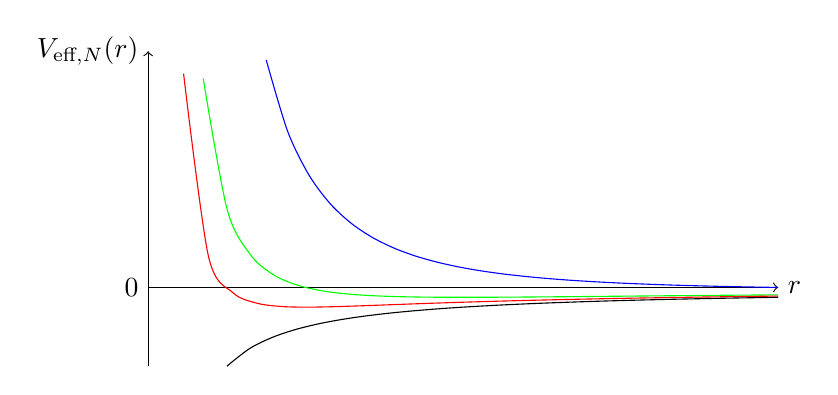
\begin{tikzpicture}
      \draw[->] (0,0) -- (8,0) node[right] {$r$};
      \draw[->] (0,-1) -- (0,3) node[left] {$V_{\text{eff},N}(r)$};
      \draw[domain=1.5:8,smooth,variable=\x,blue] plot ({\x},{-(1/\x)+8*(1/(\x*\x))});
      \draw[domain=0.7:8,smooth,variable=\x,green] plot ({\x},{-(1/\x)+2*(1/(\x*\x))});
      \draw[domain=0.45:8,smooth,variable=\x,red] plot ({\x},{-(1/\x)+(1/(\x*\x))});
      \draw[domain=1.0:8,smooth,variable=\x,black] plot ({\x},{-(1/\x)+0*(1/(\x*\x))});
      \draw (0,0) node[left]{0};
    \end{tikzpicture}
\end{center}
Plots of $V_{\text{eff},N}(r)=-\frac{\mu c^2}{r}+\frac{h^2}{r^2}$ for increasing values of $h/\mu$ (black, red, green, blue).
\begin{prop}
There are two distinct stationary points for $V_{\text{eff}}(r)$ (Eqn.~\ref{timelikeeff}) when $h>\sqrt{12}\mu c$, but only one  inflection point when $h=\sqrt{12}\mu c$. 
\end{prop}
\begin{proof}
The stationary points of $V_{\text{eff}}(r)$ can be found from
$$0=\frac{dV_{\text{eff}}}{dr}=\frac{\mu c^2}{r^2}+\frac{h^2}{r^3}\bigg(\frac{3\mu}{r}-1\bigg)\implies r_\pm=\frac{h}{2\mu c^2}(h\pm\sqrt{h^2-12\mu^2c^2})$$
Clearly, for $h>\sqrt{12}\mu c$, there will be two roots. As $h\sqrt{12}\mu c$, they merge at $r_\pm=6\mu$. No stationary points exist when $h<\sqrt{12\mu c}$.
The nature of the stationary points follow from
$$\frac{d^2V_{\text{eff}}}{dr^2}=-\frac{2\mu c^2}{r^3}+\frac{3h^2}{r^4}\bigg(1-\frac{4\mu}{r}\bigg)$$
\begin{itemize}
\item $h>\sqrt{12}\mu c$: Evaluating at $r_\pm$ gives $\frac{h^2}{r_\pm^5}(r_\pm-6\mu)$ such that $r_-$ corresponds to a local maximum and $r_+$ to a minimum. The effective potential at the stationary points evaluates to
$$V_{\text{eff}}(r_\pm)=\frac{h^2}{2r_\pm^3}(4\mu-r_\pm)$$
\item $h=\sqrt{12}\mu c$: $r=6\mu$ corresponds to an inflection point where $V_{\text{eff}}(r=6\mu)=-c^2/18$.
\end{itemize}
\end{proof}
\begin{remarks}\leavevmode
\begin{enumerate}
    \item As $h/\mu c\rightarrow\infty$, the stationary points tend to $r_+\rightarrow\infty$ and $r_-=\rightarrow 3\mu$ (from above).
    \item The reversal in sign of the centrifugal barrier at small $r$ means that a particle with sufficient energy (large enough $k$) can always reach $r=0$ for any $h$, unlike the case in Newtonian gravity. Such an in-falling particle spirals into $r=0$.
    \item For $h>\sqrt{12}\mu c$, circular orbits are possible at two radii $r_\pm$, with the innermost orbit being unstable and the outermost being stable. The radius of the unstable circular orbit is always in the range $3\mu<r_-\leq 6\mu$, while the radius of the stable circular orbit has $r_+>6\mu$. At the innermost stable circular orbit ($r=6\mu$), the particle has specific angular momentum $h=\sqrt{12}\mu c$.
    \item The circular orbits with $r>4\mu$ are bound ($k<1$, $V_{\text{eff}}<0$).
\end{enumerate}
\end{remarks}
\newpage
\begin{center}
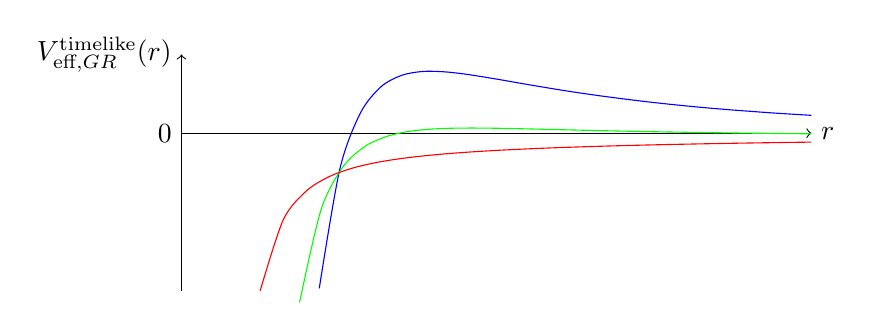
\begin{tikzpicture}
      \draw[->] (0,0) -- (8,0) node[right] {$r$};
      \draw[->] (0,-2) -- (0,1) node[left] {$V_{\text{eff},GR}^{\text{timelike}}(r)$};
      \draw[domain=1.75:8,smooth,variable=\x,blue] plot ({\x},{-(1/\x)+60*(1/(2*\x*\x)-1/(\x*\x*\x)))});
      \draw[domain=1.5:8,smooth,variable=\x,green] plot ({\x},{-(1/\x)+10*(1/(\x*\x)-2/(\x*\x*\x)))});
      \draw[domain=1.0:8,smooth,variable=\x,red] plot ({\x},{-(1/\x)+(1/(\x*\x)-2/(\x*\x*\x)))});
    \draw (0,0) node[left]{0};
    \end{tikzpicture}
\end{center}
Plots of $V_{\text{eff},GR}^{\text{timelike}}(r)=-\frac{\mu c^2}{r}+\frac{h^2}{2r^2}(1-\frac{2\mu}{r})$ for increasing values of $h/\mu$ (red, green, blue).
\begin{eg}[Accretion power]
Gas in an accretion disc around a compact object moves in quasi-circular orbits. Due to viscosity, a packet of gas in the disc loses angular momentum causing it to move slowly inwards until it can no longer follow a stable circular orbit, at which point it falls into the compact object. Vast amount of energy can be radiated as a result. The classical computation gives
$$\frac{\Delta E_N}{mc^2}=\frac{0-(-\frac{\mu}{2r}mc^2)}{mc^2}=\frac{\mu}{2r}$$
But such orbits are compact and a relativistic approach would be more accurate. The angular momentum for a circular orbit at radius $r$ follows from
$$0=\frac{dV_{\text{eff}}}{dr}=\frac{\mu c^2}{r^2}-\frac{h^2}{r^3}+\frac{3\mu h^2}{r^4}\implies\mu c^2r^2=h^2(r-3\mu)$$
but from the `energy conservation' equation, $V_{\text{eff}}(r)=\frac{1}{2}c^2(k^2-1)$. LHS is $-\frac{\mu c^2}{r}+\frac{h^2}{2r^2}(1-\frac{2\mu}{r})=-\frac{h^2}{2r^2}(1-\frac{4\mu}{r})$. This gives 
$$k=\frac{1-2\mu/r}{(1-3\mu/r)^{1/2}}$$
The particle starts in a circular orbit at $r>>\mu$, so $k\approx 1$. When it reaches $r$, the energy of the particle as measured locally by a stationary observer is ($k=1$) from Eqn.~\ref{energymassive}:
$$E_{k=1}=mc^2\bigg(1-\frac{2\mu}{r}\bigg)^{-1/2}$$
But, the energy for a particle in a circular orbit there is
$$E_{k}=kmc^2\bigg(1-\frac{2\mu}{r}\bigg)^{-1/2}=mc^2\sqrt{\frac{1-2\mu/r}{1-3\mu/r}}$$
The difference between these two energies must be lost if the particle is to enter a circular orbit at $r$, which gives
$$\frac{\Delta E}{mc^2}=\bigg(1-\frac{2\mu}{r}\bigg)^{-1/2}-\bigg(\frac{1-2\mu/r}{1-3\mu/r}\bigg)^{1/2}$$
which evaluates to $\frac{\sqrt{3}}{6}(3\sqrt{2}-4)=0.07$ at $r=6\mu$ (innermost stable circular orbit).
\end{eg}
\begin{prop}
The shape of the orbit of massive particles, in the Schwarzschild spacetime, is
\begin{equation}
\frac{d^2u}{d\phi^2}+u-3\mu u^2=\frac{\mu c^2}{h^2}\label{shapemassive}
\end{equation}
\end{prop}
\begin{proof}
The shape of the orbit is found from
\begin{equation}
\dot{r}=\dot{\phi}\frac{dr}{d\phi}=\frac{h}{r^2}\frac{dr}{d\phi}=-h\frac{du}{d\phi}\label{shape}
\end{equation}
Substitute Eqn.~\ref{shape} into Eqn.~\ref{massiveenergyeqn},
$$\frac{1}{2}h^2\bigg(\frac{du}{d\phi}\bigg)^2-GMu+\frac{h^2u^2}{2}(1-2\mu u)=\frac{1}{2}c^2(k^2-1)$$
Differentiating with respect to $\phi$, we obtain the desired equation.
\end{proof}
\subsubsection{Massless particles}
\begin{prop}
Massless particles experiences an effective potential
\begin{equation}
V^{\text{null}}_{\text{eff},GR}(r)=\frac{h^2}{2r^2}\bigg(1-\frac{2\mu}{r}\bigg)\label{masslesseffective}
\end{equation}
\end{prop}
\begin{proof}
Massless particles follow null geodesics that satisfy $Q=0$ (Eqn.~\ref{firstintegral}).
\begin{equation}
\frac{1}{2}c^2k^2=\frac{1}{2}\dot{r}^2+\frac{h^2}{2r^2}\bigg(1-\frac{2\mu}{r}\bigg):=\frac{1}{2}\dot{r}^2+V_{\text{eff}}(r)\label{masslessenergyeqn}
\end{equation}
where we followed a similar procedure as that for the derivation of Eqn.~\ref{massiveenergyeqn}.
\end{proof}
\begin{prop}
There is a single stationary point at $r=3\mu$, which maximizes the effective potential (Eqn.~\ref{masslesseffective}), i.e. $V_{\text{eff}}(3\mu)=\frac{h^2}{54\mu^2}$.
\end{prop}
\begin{proof}
The stationary points of $V_{\text{eff}}(r)$ can be found from $0=\frac{dV_{\text{eff}}}{dr}=-\frac{h^2}{r^3}(1-\frac{3\mu}{r})$ which gives $r=3\mu$. The nature of the stationary point is
$$\frac{d^2V_{\text{eff}}}{dr^2}=\frac{3h^2}{r^4}\bigg(1-\frac{4\mu}{r}\bigg)\implies\frac{d^2V_{\text{eff}}}{dr^2}\bigg|_{r=3\mu}=-\frac{h^2}{r^4}<0$$
and hence a maximum, with value $\frac{h^2}{54\mu^2}$.
\end{proof}
\begin{center}
\begin{tikzpicture}
      \draw[->] (0,0) -- (8,0) node[right] {$r$};
      \draw[->] (0,-3) -- (0,5) node[left] {$V_{\text{eff},GR}^{\text{null}}(r)$};
      \draw[domain=0.37:8,smooth,variable=\x,blue] plot ({\x},{(5/(\x*\x))-(2/(\x*\x*\x))});
      \draw[domain=0.6:8,smooth,variable=\x,green] plot ({\x},{(4/(\x*\x))-(2/(\x*\x*\x))});
      \draw[domain=0.75:8,smooth,variable=\x,red] plot ({\x},{(1/(\x*\x))-(2/(\x*\x*\x))});
    \draw (0,0) node[left]{0};
    \end{tikzpicture}
\end{center}
Plots of $V_{\text{eff},GR}^{\text{null}}(r)=\frac{h^2}{2r^2}(1-\frac{2\mu}{r})$ for increasing values of $h/\mu$ (red, green, blue).
\begin{remarks}
Massless particles have a single circular orbit at $r=3\mu$ and it is unstable.
\end{remarks}
\begin{prop}
The shape of the orbit of massless particles, in the Schwarzschild spacetime, is
\begin{equation}
\frac{d^2u}{d\phi^2}+u-3\mu u^2=0\label{shapemassless}
\end{equation}
\end{prop}
\begin{proof}
Substitute Eqn.~\ref{shape} into Eqn.~\ref{masslessenergyeqn},
$$\frac{1}{2}h^2\bigg(\frac{du}{d\phi}\bigg)^2+\frac{h^2u^2}{2}(1-2\mu u)=\frac{1}{2}c^2k^2$$
Differentiating with respect to $\phi$, we obtain the desired equation.
\end{proof}
\begin{eg}
Consider more general orbits, in particular, a photon moving inwards from large radii with angular momentum $h$. If $c^2k^2/2<V_{\text{eff}}(r=3\mu)=h^2/54\mu^2$ (Eqn.~\ref{masslessenergyeqn}), the photon cannot cross the `barrier' at the maximum point $r=3\mu$. There will be a single turning point of closest approach, where $c^2k^2/2=V_{\text{eff}}(r)$, and the photon will escape to infinity again. However, if $c^2k^2/2>V_{\text{eff}}(r=3\mu)=h^2/54\mu^2$, the photon will be captured by the massive body and will spiral inwards to $r=0$. The behaviour of the photon orbit depends on the ratio $h/k$.
To find the shape of the orbit, we have from Eqns.~\ref{conservedL} and \ref{masslessenergyeqn}.
$$\bigg(\frac{dr}{d\phi}\bigg)^2=\frac{\dot{r}^2}{\dot{\phi}^2}=\frac{r^4\dot{r}^2}{h^2}=r^2\bigg[\frac{c^2k^2}{h^2}r^2-\bigg(1-\frac{2\mu}{r}\bigg)\bigg]\approx r^2\bigg(\frac{c^2k^2r^2}{h^2}-1\bigg)$$
At large radii, the Schwarzschild metric is asymptotically flat, so we expect photon orbits to be straight line there. Define the impact parameter of the orbit to be $b$. Assume $\phi\rightarrow0$ as $r\rightarrow\infty$, the straight line path is $r\sin\phi=b$. Differentiating gives
$$\frac{dr}{d\phi}\sin\phi+r\cos\phi=0\implies\frac{dr}{d\phi}=\pm r\sqrt{\frac{r^2}{b^2}-1}\implies b=\frac{h}{ck}$$
If $b=\frac{h}{ck}<\sqrt{\frac{54\mu^2}{2}}=\sqrt{27}\mu$, the photon will be captured by the massive body.
\end{eg}
\begin{remarks}
The effects of gravitational fields on massless particles are achromatic (i.e. independent of energy). Since we have taken $p^\mu=dx^\mu/d\lambda$, considering a particle of different energy amounts to a constant scaling of the affine parameter. $k$ and $h$ will both scale in the same way, preserving their ratio.
\end{remarks}
\subsection{Gravitational redshift}
\begin{eg}[Simple example]
Consider the change in the frequency of a photon, as measured by observers at constant $(r,\theta,\phi)$, as it propagates through Schwarzschild spacetime. The energy of the photon relative to a stationary observer at $r$ is given by Eqn.~\ref{energymassless}. As $k$ is constant, if a photon is emitted at $r_E$, with frequency $\nu_E$ as measured by a stationary observer there, and is received by a stationary observer at $r_R$ who measures the frequency to be $r_E$, we have $\frac{\nu_R}{\nu_E}=\sqrt{\frac{1-2\mu/r_E}{1-2\mu/r_R}}$. \end{eg}
\begin{defi}[Redshift]
The redshift $z$ is the ratio of received to emitted wavelengths, i.e.
$1+z=\frac{\nu_E}{\nu_R}$.
\end{defi}
\begin{remarks}
For observations at infinity, the redshift becomes  $1+z_\infty=(1-\frac{2\mu}{r_E})^{-1/2}$. This is called gravitational redshift since the change in frequency of a photon is due to the gravitational field it experiences. In the weak-field limit, we have
$$1+z\approx1-\mu\bigg(\frac{1}{r_R}-\frac{1}{r_E}\bigg)=1+\frac{1}{c^2}(\Phi(r_R)-\Phi(r_E))$$
Photons loses energy when they climb out of the potential well.
\end{remarks}
\begin{prop}
For an arbitrary static metric, the gravitational redshift generalizes to
\begin{equation}
\frac{\nu_R}{\nu_E}=\sqrt{\frac{g_{00}(E)}{g_{00}(R)}}\label{gravitationalredshift}
\end{equation}
\end{prop}
\begin{proof}
For any static metric, we have the Lagrangian to be
$$\hat{\mathcal{L}}=g_{00}\dot{t}^2+\sum_{ij}g_{ij}\dot{x}^i\dot{x}^j$$
where the metric functions are time-independent. The Euler-Lagrange equations for $t$ now gives $g_{00}\dot{t}=$const. (since $\partial\hat{\mathcal{L}}/\partial t=0$. But, the 4-velocity of a stationary observer is $u^\mu=\frac{c}{\sqrt{g_00}}(1,\vec{0})$. The energy of the photon as measured by such an observer is
$$E=g_{00}\frac{c}{\sqrt{g_{00}}}\dot{t}\propto\frac{1}{\sqrt{g_{00}}}$$
This gives the desired formula for the gravitational redshift.
\end{proof}
\newpage
\section{Classic tests of General Relativity}
\subsection{Mercury's perihelion precession}
\begin{prop}[Newtonian Attempt]
The equation of orbit is
\begin{equation}
u=\frac{\mu c^2}{h^2}(1+e\cos\phi),\quad\mu=\frac{GM}{c^2}\label{NewtonianConic}
\end{equation}
where $u=\frac{1}{r}$ and $\phi$ is the usual angular coordinate. For eccentricity $e<1$, the orbit will be an ellipse.
\end{prop}
\begin{proof}
Using energy conservation in the classical picture:
$$E_N=\frac{1}{2}m\dot{r}^2+\frac{1}{2}mr^2\dot{\phi}^2-\frac{\mu c^2m}{r}=\frac{1}{2}mh^2\bigg(\frac{du}{d\phi}\bigg)^2+\frac{1}{2}h^2mu^2-\mu c^2 mu\implies 0=\frac{du}{d\phi}\bigg[\frac{d^2u}{d\phi^2}+u-\frac{\mu c^2}{h^2}\bigg]$$
where we used Eqn.~\ref{shape}, $\dot{\phi}=h/r^2$ and $u=1/r$. The equation may be solved by Eqn.~\ref{NewtonianConic}.
\end{proof}
\begin{remarks}\leavevmode
\begin{enumerate}
\item We may relate the eccentricity $e$ to the energy $E_N$ and the semi-major axis of the ellipse $a=\frac{h^2}{GM(1-e^2)}$
\begin{equation}
 \frac{E_N}{mh^2}=\frac{1}{2}\bigg(\frac{\mu c^2}{h^2}\bigg)^2(e^2-1)=-\frac{GM}{2a}\frac{1}{h^2}\label{axes}
\end{equation}
\item The Newtonian solution is not able to account for the precession of Mercury's perihelion.
\end{enumerate}
\end{remarks}
\begin{prop}[Relativistic Attempt]
The equation of orbit for a massive particle in the Schwarzschild metric is approximately
\begin{equation}
u\approx\frac{\mu c^2}{h^2}(1+e\cos[\phi(1-\alpha)])\label{relorbitsol}
\end{equation}
where $u=\frac{1}{r}$ up to order $O(\alpha)$ such that $\alpha:=\frac{3\mu^2c^2}{h^2}<<1$ is small.
\end{prop}
\begin{proof}
The shape of the orbit for a massive particle in the Schwarzschild metric is given by Eqn.~\ref{shapemassive}. In the limit of weak relativistic correction ($\mu<<r$), we may use perturbation theory. We remove the dimensions of $u$ via $u=\frac{\mu c^2}{h^2}U$ such that the equation is now
$$\frac{d^2U}{d\phi^2}+U=1+\alpha U^2,\quad\alpha=\frac{3\mu^2c^2}{h^2}=\frac{3\mu}{r_0}$$
where $r_0=\frac{h^2}{GM}$ is the radius of the stable Newtonian circular orbit. Try solution $U=U_0+\alpha U_1+\alpha^2U_2+\dots$
$$O(1):\quad\frac{d^2U_0}{d\phi^2}+U_0-1=-e\cos\phi+(1+e\cos\phi)-1=0$$
$$O(\alpha):\quad\frac{d^2U_1}{d\phi^2}+U_1=(1+e\cos\phi)^2=1+\frac{1}{2}e^2+2e\cos\phi+\frac{1}{2}e^2\cos2\phi$$
The particular integral is solved by guessing $U_1(\phi)=A+B\phi\sin\phi+C\cos(2\phi)$ which upon solving, gives $A=1+\frac{1}{2}e^2$, $B=e$, $C=\frac{1}{6}e^2$. The term $\phi\sin\phi$ will grow over many orbits, so the approximate orbit solution is
$$u(\phi)\approx\frac{\mu c^2}{h^2}(1+e\cos\phi+e\alpha\phi\sin\phi)\approx\frac{\mu c^2}{h^2}(1+e(\cos\phi\cos\alpha\phi+\sin\phi\sin\alpha\phi))\approx\frac{\mu c^2}{h^2}(1+e\cos(\phi(1-\alpha)))$$
\end{proof}
\begin{remarks}
$u(\phi)\sim1+e\cos[\phi(1-\alpha)]$ is no longer a closed orbit, and the ellipse precesses with the angle $\phi$ at perihelion increasing by $\Delta\phi=2\pi(\frac{1}{1-\alpha}-1)\approx 2\pi\alpha=\frac{6\pi GM}{c^2}\frac{1}{a(1-e^2)}$ per revolution.
\end{remarks}
\begin{eg}
Using $M$ as the mass of the Sun, the perihelion precession rate of Mercury is
$$\frac{\Delta\phi}{T}=\frac{6\pi GM}{a(1-e^2)c^2T}=\frac{6\pi(6.67\times10^{-11})(2\times10^{30})}{(5.8\times10^{10})(1-0.21^2)(3\times10^8)^2}\sim \frac{5.04\times10^{-7}\text{rad}}{88\text{days}}=\frac{5.04\times10^{-7}\times 60^2\times(360/2\pi)}{88/(365.25\times100)}$$
which is 43.1 arc seconds per century for Mercury, as testified by observations. Here, $\alpha<<1$ indeed.
\end{eg}
\subsection{Gravitational lensing}
\begin{prop}[Newtonian Attempt]
The total deflection predicted is $\frac{2GM}{bc^2}$.
\end{prop}
\begin{proof}
In the absence of gravitational field, we have $\frac{d^2u}{d\phi^2}+u=0\implies u=\frac{1}{b}\sin\phi$ where $b$ is physically the impact parameter. Light goes from the left $(\phi\rightarrow\pi)$ to right $(\phi\rightarrow 0)$. With the field, we recall from Mercury perihelion precession that $u\approx\frac{\mu c^2}{h^2}(1+e\sin\phi)$, up to a phase difference. Consider a small deflection. $u=0$ at $\phi=-\Delta\phi$ and $\pi+\Delta\phi$ with $\Delta\phi<<1$. Then, $\sin(-\Delta\phi)\approx-\Delta\phi=-\frac{1}{e}$ and $\sin(\pi+\Delta\phi)\approx-\Delta\phi=-\frac{1}{e}$. It follows $\frac{1}{e}<<1$ and so $e>>1$. The impact parameter is $\frac{1}{b}=u(\pi/2)=\frac{\mu c^2}{h^2}(1+e)\approx\frac{\mu c^2e}{h^2}$. The angular momentum is $h=cb$. The total deflection will be $2\Delta\phi=\frac{2}{e}=\frac{2\mu c^2b}{h^2}=\frac{2GM}{c^2b}$.
\end{proof}
\begin{figure}[H]
    \centering
    \includegraphics[width=\linewidth]{deflection.PNG}
    \caption{Light bending in the (left) absence (right) presence of gravitational field. Image credit: U. Spearhake}
\end{figure}
\begin{prop}[Relativistic Attempt]
The total deflection predicted is $\frac{4GM}{c^2b}$.
\end{prop}
\begin{proof}
The shape of a massless particle in the Schwarzschild metric is given by Eqn.~\ref{shapemassless}. In the absence of a field, $M=0$ and we recover the limit $u=\frac{1}{b}\sin\phi$. Consider small deflection such that using perturbation theory, we have $bu=\sin\phi+\beta U_1+\beta^2U_2$, where again $u=\frac{\mu c^2}{h^2}U$. Plug this into Eqn.~\ref{shapemassless}, the $O(1)$ terms consistently cancel out, while
$$O(\beta):\quad\frac{d^2U_1}{d\phi^2}+U_1=\sin^2\phi=\frac{1}{2}(1-\cos2\phi)$$
We guess the full solution to be $U_1(\phi)=C_1\sin\phi+C_2\cos\phi+C_3\cos2\phi+C_4$. $C_3$ and $C_4$ are obtained by substituting this guess $\implies C_3=\frac{1}{6}$, $C_4=\frac{1}{2}$. $C_1$ and $C_2$ are recovered in the asymptotic limit, i.e. $bu\rightarrow\sin\phi$ as $\phi\rightarrow\pi$, so $C_1=0$ and $C_2=\frac{2}{3}$.
At the far end of the light path, $u\rightarrow 0$ as $\phi\rightarrow-\Delta\phi$ where $|\Delta\phi|<<1$. We thus have
$$0\approx-\frac{\Delta\phi}{b}+\frac{3GM}{c^2b^2}\frac{4}{3}$$
\end{proof}
\begin{remarks}
The result predicted by relativity is twice that of the Newtonian result.
\end{remarks}
\begin{eg}
The light deflection by the Sun is measured during the 1919 solar eclipse by Arthur Eddington. For $b=7\times10^8$ m, this is
$$\frac{4(6.67\times10^{-11})(2\times10^{30})}{9\times10^{16}(7\times10^8)}\times\frac{360}{2\pi}\times 60^2=1.75''$$
\end{eg}
\newpage
\section{Schwarzschild black holes}
\subsection{Causal structure}
\begin{remarks}
The Schwarzschild metric (Eqn.~\ref{Schwarzschild}) is singular at $r=0$ and $r=2\mu$. $r=2\mu$ is a coordinate singularity while $r=0$ is not. 
\end{remarks}
\begin{defi}[Schwarzschild radius]
We define the Schwarzschild radius to be $r_s=2\mu=\frac{2GM}{c^2}$. The Schwarzschild radius is important if the radius of the body is less than $r_s$, i.e. compact.
\end{defi}
To investigate the nature of the singularities, we should consider coordinate-independent properties. One way is to form invariants using the Riemann curvature tensor.
\begin{defi}[Kretschmann scalar]
To determine if a singularity is physical, we compute the Kretschmann scalar at that point $R_{\mu\nu\rho\sigma}R^{\mu\nu\rho\sigma}$.  
\end{defi}
\begin{eg}
For the Schwarzschild metric, \begin{equation}
R_{\mu\nu\rho\sigma}R^{\mu\nu\rho\sigma}\propto\frac{\mu^2}{r^6}\label{Kretschmann}
\end{equation}
and it is related to the magnitude of tidal effects. The Kretschmann scalar is regular at $r=2\mu$ but singular at $r=0$. $r=0$ is a true singularity.
\end{eg}
\begin{eg}[Coordinate singularity]
Consider a 2-sphere, of radius $a$, described in cylindrical coordinates $(\rho,\phi)$, which has an induced line element of 
$$ds^2=\frac{a^2d\rho^2}{a^2-\rho^2}+\rho^2d\phi^2$$
The metric is singular at $\rho=a$, but we know the 2-sphere is perfectly regular everywhere, including the equator. The coordinate invariants are all regular (and same everywhere) and hence $\rho=a$ is a coordinate singularity.
\end{eg}
For the Schwarzschild metric, the boundary $r=2\mu$ demarcates two distinct regions.
\begin{prop}
The radial and time coordinates have opposite behaviours in $r<2\mu$ and $r>2\mu$.
\end{prop}
\begin{proof}
When $r>2\mu$, the coordinate basis vector $\mathbf{e_0}=\partial/\partial t$ is timelike:
$$g(\mathbf{e_0},\mathbf{e_0})=g_{00}=c^2\bigg(1-\frac{2\mu}{r}\bigg)>0$$
i.e. a curve at constant $(r,\theta,\phi)$ is timelike. The spatial basis vectors, here are spacelike. On the contrary, when $r<2\mu$, $g(\mathbf{e_0},\mathbf{e_0})<0$ and so the $\mathbf{e_0}$ basis vector is spacelike, but the spatial basis vectors are timelike. 
\end{proof}
\begin{defi}[Region type]
Colloquially, we can refer the regions when the spatial basis vectors are spacelike (timelike) to be of Type I (Type II).
\end{defi}
\subsubsection{Light cones}
\begin{remarks}
Light cones provide a useful tool to understand the causal structure of spacetime since they represent the possible trajectories of null curves and the boundary of timelike curves which must be inside the light cones. Future (past)-pointing light cones open up into $t>0$ ($t<0$).
\end{remarks}
We construct the light cones in Schwarzschild spacetime from radial null geodesics ($d\theta=0=d\phi$).
\begin{prop}
The radial null geodesics are described by
\begin{equation}
    ct(r)=\pm(r+2\mu\ln|r-2\mu|)+C,\quad C=\text{const.}\label{radialnull}
\end{equation}
\end{prop}
\begin{proof}
From Schwarzschild metric (Eqn.~\ref{Schwarzschild}), we have
$$\frac{dct}{dr}=\pm\bigg(1-\frac{2\mu}{r}\bigg)^{-1}=\pm1\pm\frac{1}{(r/2\mu)-1}\implies ct=\pm r\pm2\mu\ln\bigg|\frac{r}{2\mu}-1\bigg|+C$$
where $C$ is constant. The absolute value means we can consider both $r>2\mu$ and $r<2\mu$. In either region, there are a family of outgoing and ingoing radial null geodesics, given by the positive and negative branch of the solution. 
\end{proof}
\begin{remarks}\leavevmode
\begin{enumerate}
    \item The Schwarzschild metric is symmetric under time reversal (i.e. static) $\implies$ the ingoing and outgoing radial null geodesic solutions are related by $t\rightarrow -t$.
    \item The Schwarzschild metric is asymptotically flat $\implies$ the radial null geodesics are straight lines of gradient $\pm1$ for $r>>2\mu$.
    \item It takes an infinite coordinate time for an ingoing photon to reach $r=2\mu$.
    \item All outgoing rays seem to originate from $r=2\mu$ and $ct\rightarrow-\infty$.
\end{enumerate}
\end{remarks}
We now draw the light cone structure of the Schwarzschild solution.
\begin{figure}[H]
    \centering
    \includegraphics[scale=0.5]{radialnull.PNG}
    \caption{Ingoing (orange) and outgoing (blue) radial null geodesics are discontinuous at $r=2M$ (natural units). Also included are the future-pointing light cones, in green. Image credit: U. Spearhake}
\end{figure}
\begin{itemize}
\item For $r>2\mu$: $r=$const. curves have time-like ($g(\mathbf{e_0},\mathbf{e_0})>0$) behaviour and thus the light cones open up towards $t>0$.
\item For $r<2\mu$: $t=$const. curves have time-like ($g(\mathbf{e_r},\mathbf{e_r})>0$) behaviour and thus the light cones are tilted horizontally. Physically, the gravitational field pulls object towards the centre, so we could expect the future light cones to point towards $r=0$.
\end{itemize}
\begin{prop}
With a finite change in its affine parameter, an ingoing photon may cross $r=2\mu$.
\end{prop}
\begin{proof}
From Eqn.~\ref{conservedE}, we have 
$$\frac{dr}{d\lambda}=\frac{dr}{dt}\frac{dt}{d\lambda}=k\frac{dr}{dt}\bigg(1-\frac{2\mu}{r}\bigg)^{-1}=\pm kc\implies r=\pm ck\lambda+C$$
where $\lambda$ is an affine parameter, and $\frac{dct}{dr}=\pm(1-2\mu/r)^{-1}$ (from Schwarzschild metric Eqn.~\ref{Schwarzschild}).
\end{proof}
\begin{remarks}
Future-directed ingoing null geodesics in the region $r>2\mu$ reach $r=2\mu$ and $t=\infty$ at a finite value of their affine parameter, and then extend into the region $r<2\mu$ moving towards $r=0$ with decreasing $t$. Region $r<2\mu$ is a Type II region since the light cones are tipped over towards $r=0$. The region II in the causal future of region I is a black hole.
\end{remarks}
\begin{defi}[Black hole]
A black hole is a region of spacetime from which no particle can escape to spatial infinity.
\end{defi}
\begin{remarks}
Outgoing null geodesics in the region $r>2\mu$ may cross to $r<2\mu$ upon a change in affine parameter. If we try and extend such outgoing geodesics back to smaller values of $\lambda$, we find that they join onto geodesics in $r<2\mu$ that have $r$ increasing with $\lambda$ and $t$ decreasing. But now, the forward light cone is directed away from $r=0$, this is a type II region (different from causal future) that is the causal past of region I. All particles are inevitably expelled to $r>2\mu$.
\end{remarks}
\begin{defi}[White hole]
A white hole is a region of spacetime from which all particles are inevitably expelled to spatial infinity.
\end{defi}
\begin{prop}
It takes an infinite coordinate time for a massive infalling particle to reach $r=2\mu$. Coordinate time refers to the proper time of an observer far away from $r=2\mu$.
\end{prop}
\begin{proof}
Differentiate Eqn.~\ref{massiveenergyeqn} (for massive particles) with respect to proper time $\tau$, to obtain
$$\ddot{r}=-\frac{GM}{r^2}$$
Consider a particle that starts at rest at infinity, so that $k=1$. For an in-falling particle, 
$$\dot{r}=-\sqrt{2\mu c^2/r}\implies c(\tau-\tau_0)=\frac{2}{3\sqrt{2\mu}}(r_0^{3/2}-r^{3/2})$$
It takes finite amount of proper time to reach $r=2\mu$ and $r=0$. To determine the coordinate time, we have
\begin{align}
\frac{dct}{dr}&=c\frac{\dot{t}}{\dot{r}}=-\sqrt{\frac{r}{2\mu}}\bigg(1-\frac{2\mu}{r}\bigg)^{-1}\nonumber\\\implies c(t-t_0)&=-2\mu\int_{r_0/2\mu}^{r/2\mu}\frac{x^{3/2}}{x-1}dx\nonumber\\&=-2\mu\bigg[\frac{2}{3}x^{3/2}+2\sqrt{x}+\ln\bigg|\frac{\sqrt{x}-1}{\sqrt{x}+1}\bigg|\bigg]_{r_0/2\mu}^{r/2\mu}\nonumber\\&=-2\mu\bigg\{\frac{2}{3(2\mu)^{3/2}}(r^{3/2}-r_0^{3/2})+\frac{2}{\sqrt{2\mu}}(\sqrt{r}-\sqrt{r_0})+\ln\bigg|\frac{(\sqrt{r/2\mu}-1)(\sqrt{r_0/2\mu}+1)}{(\sqrt{r_0/2\mu}-1)(\sqrt{r/2\mu}+1)}\bigg|\bigg\}\nonumber
\end{align}
The integral is improper as $r\rightarrow 2\mu$, i.e. $t\rightarrow\infty$. 
\end{proof}
\begin{figure}[H]
    \centering
    \includegraphics[scale=0.7]{radialtimelike.PNG}
    \caption{The proper time (blue) and coordinate time (red) for radial time-like geodesics for a massive infalling observer. The coordinate time has a vertical asymptote at $r=2M$ (natural units. For smaller $r<2M$, the coordinate time decreases with increasing $\tau$ (not plotted). The infalling observer will reach the singularity at $r=0$ after some finite $\tau$. Image credit: U. Spearhake}
\end{figure}
\begin{remarks}
Consider the in-falling particle as observed by a stationary observer ar $r=\infty$. Light from the particle only reaches the distant observer if it is emitted at $r>2\mu$. Since the coordinate time $t$ is the proper time for the distant observer, they perceive that it takes an infinite amount of their proper time for the particle to reach $r=2\mu$ from any finite $r>2\mu$. The light signals emitted as $r\rightarrow 2\mu$ are also infinitely redshifted when they reach the distant observer. 
\end{remarks}
\subsubsection{Eddington Finkelstein Coordinates}
\begin{remarks}
We attempt to construct coordinates that cover both regions $r<2\mu$ and $r>2\mu$ in its causal future without coordinate singularities. The coordinates are adapted to radially-infalling photons in such a way that their worldlines are continuous through $r=2\mu$.
\end{remarks}
The form of the ingoing radial null geodesics ($t+2\mu\ln|r-2\mu|=-r+C$) motivates the following coordinate choice:
\begin{defi}[Ingoing Eddington Finkelstein coordinates (IEF)]
$$ct_{\text{IEF}}:=ct+2\mu\ln|r-2\mu|$$
In this new coordinates, the outgoing and ingoing radial null geodesics now become
$$ct_{\text{IEF}}=r+4\mu\ln|r-2\mu|+C,\quad ct_{\text{IEF}}=-r+C$$
\end{defi}
Similarly, the outgoing radial null geodesics ($t-2\mu\ln|r-2\mu|=r+C$) gives rise to 
\begin{defi}[Outgoing Eddington Finkelstein coordinates (OEF)]
$$ct_{\text{OEF}}:=ct-2\mu\ln|r-2\mu|$$
In this new coordinates, the outgoing and ingoing radial null geodesics now become
$$ct_{\text{OEF}}=r+C,\quad ct_{\text{OEF}}=-r-4\mu-\ln|r-2\mu|+C$$
\end{defi}
The light cone structure of the Schwarzschild solutions, in the respective new coordinates.
\begin{figure}[H]
\begin{minipage}{\linewidth}
\subfloat[]{\includegraphics[width=.5\linewidth]{IEF.PNG}}
\subfloat[]{\includegraphics[width=0.5\linewidth]{OEF.PNG}}
\end{minipage}
    \caption{IEF (left) and OEF (right). Again, ingoing and outgoing radial null geodesics are coloured orange and blue respectively, while future-pointing light cones are in green. Image credit: U. Spearhake}
\end{figure}
\newpage
\begin{remarks}\leavevmode
\begin{enumerate}
    \item In either coordinate choice, the light cones now smoothly vary across $r=2\mu$. In the $r\rightarrow\infty$ limit, the metric is asymptotically flat and the light cones approach their Minkowskian structure with 45 degrees inclination.
    \item For the IEF, they tilt over in the inward direction, in the black hole, such that outgoing null geodesics, in $r<2\mu$, are directed towards decreasing $r$. Similarly, for the OEF, all outgoing light rays now always point outwards at 45 degrees, and ingoing null geodesics, in $r<2\mu$ (white hole region), will point towards increasing $r$.
    \item For the IEF, the outgoing geodesics in $r>2\mu$ are still discontinuous at $r=2\mu$. This is because the causal past of $r>2\mu$ is another type II region, but with the character of a white hole rather than a black hole. The IEF do not cover this type II region.
    \item The OEF aims to cover this type II region, but it does not cover the black hole region (causal future of $r>2\mu$ region).
    \item $r=2\mu$ behaves like a one-way membrane such that light rays can move towards $r<2\mu$ from the outside, but not the other way round. Even outgoing light rays are drawn in by the gravitational field. Since timelike curves are bounded by light cones, timelike observers inside $r<2\mu$ also inevitably fall towards smaller $r$.
\end{enumerate}
\end{remarks}
The $r=2\mu$ hypersurface defines the event horizon.
\begin{defi}[Event Horizon]
The outermost boundary of a region of spacetime from which no null geodesics or timelike curves can escape to infinity.
\end{defi}
\begin{prop}
In the IEF and OEF respectively, the Schwarzschild metric (Eqn.~\ref{Schwarzschild}) becomes
$$ds^2=c^2\bigg(1-\frac{2\mu}{r}\bigg)dt_{\text{IEF}}^2-\frac{4\mu c}{r}dt_{\text{IEF}}dr-\bigg(1+\frac{2\mu}{r}\bigg)dr^2-r^2d\Omega^2$$
$$ds^2=c^2\bigg(1-\frac{2\mu}{r}\bigg)dt_{\text{OEF}}^2+\frac{4\mu c}{r}dt_{\text{OEF}}dr-\bigg(1+\frac{2\mu}{r}\bigg)dr^2-r^2d\Omega^2$$
\end{prop}
\begin{proof}
The corresponding infinitesimal time gives
$$cdt_{\text{IEF}}=cdt+\bigg(\frac{r}{2\mu}-1\bigg)^{-1}dr,\quad cdt_{\text{OEF}}=cdt-\bigg(\frac{r}{2\mu}-1\bigg)^{-1}dr$$
Rearrange to bring $cdt$ as the subject and plug into Eqn.~\ref{Schwarzschild}. Simplifying them gives the desired result.
\end{proof}
\begin{remarks}
This is no longer singular at $r=2\mu$ and is regular for the whole range $0<r<\infty$. The time component of the metric does vanish at $r=2\mu$, but this is not problematic since the metric is non-diagonal and so the determinant is still non-zero and an inverse exists.
\end{remarks}
\begin{remarks}[Kruskal-Szekeres Coordinates]
The tilting of the light cones in either EF coordinates seemingly contradicts the time reversal symmetry for a static spacetime. It is possible to combine the ingoing and outgoing Eddington-Finkelstein coordinates to form the Kruskal-Szekeres coordinates that cover the global spacetime in a non-singular way.\\[5pt]
In the new coordinates, the radial null geodesics now have a simple form $\hat{t}=\pm\hat{r}+C$. The singularity at $r=2\mu$ and $r=0$ becomes $\hat{t}=\pm\hat{r}$ (null surface) and $\hat{t}=\pm\sqrt{\hat{r}^2+2\mu}$ ($\hat{t}$ has to satisfy $\hat{t}^2\leq\hat{r}^2+2\mu$) respectively. The singularity at $r=0$ is now spacelike. Constant $r$ and constant $t$ surfaces are represented by hyperbolae and $\hat{t}\propto\hat{r}$. Now, $\hat{t}\in(-\infty,\infty)$, but these two asymptotically flat regions are causally
disconnected.
\end{remarks}
\newpage
\subsection{Formation of black holes}
As a toy model for the formation of a black hole, consider the spherically-symmetric collapse of a cloud of pressure-free dust. 
\begin{eg}[Spherical symmetric collapse of dust]
Without pressure support, the dust follows geodesics in spacetime. By Birkhoff's theorem, the spacetime outside the dust cloud will be described by the Schwarzschild solution, so we can treat the outside edge of the cloud as a massive particle free-falling radially in Schwarzschild spacetime.\\[5pt]
For simplicity, we shall assume that the collapse starts from rest at infinity ($k=1$). A distant ($r>>2\mu$) stationary observer will never see the surface of the dust cloud pass through $r=2\mu$. Light emitted after the surface crosses $r=2\mu$ will instead end up at the singularity at $r=0$. The light is increasingly redshifted as $r\rightarrow 2\mu$ and the arrival rate of photons (become dimmer) as measured by the distant observer fall to zero.\\[5pt]
Before the surface of the star crosses $r=2\mu$, we can describe the collapse in terms of the standard Schwarzschild coordinates $(t,r,\theta,\phi)$. Suppose the edge of the cloud emits a radially outgoing photon at coordinates $(t_E,r_E)$ which is received at $(t_R,r_R)$ by the distant stationary observer. Since these coordinates lie on an outgoing null geodesic (Eqn.~\ref{radialnull}), we have
$$ct_R-r_R-2\mu\ln\bigg(\frac{r_R}{2\mu}-1\bigg)=ct_E-r_E-2\mu\ln\bigg(\frac{r_E}{2\mu}-1\bigg)$$
The relation between $ct_E$ and $r_E$ is given by the path of the edge of the dust cloud. As $r_E\rightarrow 2\mu$, we have
$$ct_E=2\mu\ln\bigg(\frac{\sqrt{r_E/2\mu}+1}{\sqrt{r_E/2\mu}-1}\bigg)+C$$
We then have
$$ct_R\rightarrow 2\mu\ln\bigg(\frac{\sqrt{r_E/2\mu}+1}{\sqrt{r_E/2\mu}-1}\bigg)-2\mu\ln\bigg(\frac{r_E}{2\mu}-1\bigg)+C\approx-4\mu\ln\bigg(\frac{r_E}{2\mu}-1\bigg)+C\implies r_E(t_R)-2\mu\propto e^{-ct_R/4\mu}$$
The radius of the cloud has when observed at $t_R$ approaches $r=2\mu$ exponentially with characteristic time $4\mu/c$. We can also compute the redshift of the light from the surface. We have $\frac{\nu_R}{\nu_E}=\frac{g(p_R,u_R)}{g(p_E,u_E)}$, where $p_E$ is the 4-momentum of a radial outgoing photon at emission at $r_E$, and similarly for $p_R$, and $u_E$ is the 4-velocity of the edge of the dust cloud at $r_E$ and $u_R$ is the 4-velocity of the distant observer. The 4-velocity for a static observer at $r\rightarrow\infty$ is $u_R^\mu=(1,\vec{0})$. The 4-velocity of a cloud starting from rest at infinity ($k=1$, Eqn.~\ref{conservedE} and $\frac{d^2r}{d\tau^2}=-GM/r^2$) and the 4-momentum of a radial outgoing photon are respectively,
$$u_E^\mu=\bigg(\frac{dt}{d\tau},\frac{dr}{d\tau},0,0\bigg)=\bigg((1-2\mu/r_E)^{-1},-\sqrt{\frac{2\mu c^2}{r_E}},0,0\bigg),\quad p^\mu=\bigg(\frac{dt}{d\lambda},\frac{dr}{d\lambda},0,0\bigg)=\frac{dt}{d\lambda}\bigg(1,c\bigg(1-\frac{2\mu}{r}\bigg),0,0\bigg)$$
where $g_{\mu\nu}p^\mu p^\nu=0$. Using Eqn.~\ref{Schwarzschild}, the frequencies are
$$\nu_R=g_{00}u^0_Rp^0_R=\bigg(1-\frac{2\mu}{r}\bigg)c^2\frac{dt}{d\lambda}$$
$$\nu_E=g_{00}u_E^0p_E^0+g_{11}u_E^1p_E^1=\bigg(1-\frac{2\mu}{r}\bigg)\frac{dt}{d\lambda}\bigg[c^2\bigg(1-\frac{2\mu}{r}\bigg)^{-1}+\bigg(1-\frac{2\mu}{r}\bigg)^{-1}\sqrt{\frac{2\mu c^2}{r}}c\bigg]=c^2\frac{dt}{d\lambda}\bigg(1+\sqrt{\frac{2\mu}{r}}\bigg)$$
$$\implies\frac{\nu_R}{\nu_E}=1-\sqrt{\frac{2\mu}{r_E}}\sim 1-(1+a\exp(-ct_R/4\mu))^{-1/2}\sim\frac{1}{2}a\exp(-ct_R/4\mu)$$
where $a$ is some unimportant constant. The observed frequency decreases exponentially with characteristic decay time $4\mu/c$.
\end{eg}
\begin{eg}
After a star has expended its nuclear fuel, it will cool and lose pressure support causing it to contract under the influence of gravity. If the star is sufficiently massive and contracts to a radius smaller than $2GM/c^2$, it must inevitably collapse to form a singularity resulting in a black hole.
\end{eg}
\newpage
\section{Cosmology}
We now aim to use relativistic models to describe our entire Universe.
\begin{remarks}\leavevmode
\begin{enumerate}
\item Over large spatial scales, the Universe appears spatially homogeneous and isotropic around every point. This is supported by astrophysical observations, notably the cosmic microwave background radiation (CMBR). This provides us with sufficient degrees of symmetry, allowing us to find analytic solutions. The structures we observe on smaller scales treated as perturbation to the highly symmetric background.
\item We can model matter of Universe as a fluid, i.e continuum limit of a large number of particles.
\item A homogeneous Universe with constant magnetic field everywhere is not isotropic. Conversely, an isotropic Universe is not necessarily homogeneous.
\end{enumerate}
\end{remarks}
\subsection{Homogeneity and isotropy}
\begin{post}[Cosmological Principle]
The Cosmological Principle states that at a given time, the Unvierse is spatially homogeneous and isotropic when viewed on large scales. 
\end{post}
\begin{defi}[Fundamental observers]
If we assume that we are not in a privileged location, then it should be possible to construct a whole class of observers (we named them `fundamental observers'), filling space, who all observe the Universe to be isotropic. Moreover, with appropriate synchronisation of their clocks, the fundamental observers must agree on what they observe at any given proper time, hence spatially homogeneous.
\end{defi}
\begin{defi}[Synchronous Coordinates]
Let $x^i$ be the spatial coordinates co-moving with the cosmological fluid (i.e. that of the fundamental observers). The worldlines of fundamental observers are of the form $x^\mu=(t,x^i)$, where $x^i=$const. for each observer. We label the surfaces of homogeneity with proper time as measured by one of the fundamental observers. Let $x^0=t$ be the proper time along the world lines of the cosmological fluid. The line element in these synchronous coordinates must take the following form:
\begin{equation}
    ds^2=c^2dt^2+g_{ij}(t,\vec{x})dx^idx^j\label{synchronous}
\end{equation}
\end{defi}
\begin{post}[Weyl's Postulate]
The world lines of the Universe's fluid elements (and hence that of the fundamental observers) are orthogonal to hypersurfaces of constant time, $\Sigma_t$, to which the cosmological principle applies.
\end{post}
\begin{remarks}\leavevmode
\begin{enumerate}
    \item Fundamental observers must comove with the matter in the Universe, staying in fixed positions in comoving coordinates. They must not have peculiar motion relative to the average large-scale motion of the cosmological fluid elements, otherwise the 3-velocity of the matter they measure locally would break isotropy.
    \item Fundamental observers must be free-falling. If they were accelerating, their motion will depart from geodesics, hence breaking isotropy.
    \item Local measurements of the density in the instantaneous rest space of each fundamental observer must reveal no spatial gradients (otherwise they will break isotropy), so the local rest spaces must be tangent to the hypersurfaces of constant density. Pressure gradients in the instantaneous rest space of the fluid, would also result in acceleration.
    \item We do not require homogeneity in time.
    \item By spatial homogeneity, all fundamental observers will see cosmic time pass at the same rate as their proper time.
\end{enumerate}
\end{remarks}
\newpage
\begin{cor}\leavevmode
\begin{enumerate}
    \item $t=\tau$ where $\tau$ is the proper time for the observer.
    \item $g_{0i}=0$.
    \item the worldlines $x^\mu=(t,x^i)$ for fixed $x^i$ are geodesics.
\end{enumerate}
\end{cor}
\begin{proof}\leavevmode
\begin{enumerate}
    \item By construction, $dx^\mu=\tensor*{\delta}{*_{}^{\mu}_{0}}dt$ along the worldline, so Eqn.~\ref{synchronous} gives $c^2d\tau^2=ds^2=c^2dt^2\implies t=\tau$.
    \item $e_0$ is tangent to the worldlines of comoving observers since they are curves $x^i=$const. By Weyl's postulate, any infinitesimal displacement in the hypersurface $t=$const. is of the form $dx^\mu=(0,dx^i)$, and this must be orthogonal everywhere to the 4velocity of the fundamental observers, $u^\mu=\tensor*{\delta}{*_{}^{\mu}_{0}}$ since $e_i$ is tangent to the hypersurface. We must have $g_{0i}=0$.
    \item $t=\tau$ is an affine parameter, so we require
    $$0=\frac{d^2x^\mu}{dt^2}+\Gamma^\mu_{\nu\rho}\frac{dx^\nu}{dt}\frac{dx^\rho}{dt}=0+\Gamma_{00}^\mu$$
    Eqn.~\ref{synchronous} does satisfy this since $\Gamma_{00}^\mu=\frac{1}{2}g^{\mu\nu}(2\partial_0g_{\nu0}-\partial_\nu g_{00})=\frac{1}{2}g^{\mu\nu}(2\partial_00-\partial_\nu c^2)=0$.
\end{enumerate}
\end{proof}
\begin{prop}[Robertson-Walker-Metric]
\begin{equation}
ds^2=c^2dt^2-a(t)^2\bigg[\frac{dr^2}{1-kr^2}+r^2(d\theta^2+\sin^2\theta d\phi^2)\bigg]\label{RWM}
\end{equation}
\end{prop}
\begin{proof}
The intrinsic geometry must be consistent with isotropy and homogeneity $\forall t$, if every component of $g_{ij}$ evolves in the same way with $t$, so we write
\begin{equation}
g_{ij}(t,\vec{x})=-a^2(t)h_{ij}(\vec{x})\label{scale}
\end{equation}
where $a(t)$ is the scale factor which determines the overall scale of the intrinsic geometry of the $t=$const. surfaces, $h_{ij}(\vec{x})$ is the 3D metric of the surfaces $t=$const. Under time-independent coordinate transformations, $x^i\rightarrow x'^i(\vec{x})$ in spacetime, $h_{ij}$ transform as a 3D type (0,2) tensor.\\[5pt]
We require $h_{ij}$ to describe a homogeneous and isotropic (hence spherically symmetric) 3D space. Let $h_{ij}dx^idx^j=B(r)dr^2+r^2d\Omega^2$, then it follows that
$$h_{rr}=B(r),\quad h_{\theta\theta}=r^2,\quad h_{\phi\phi}=r^2\sin^2\theta$$
The following quantities are restricted to 3D space. The connection coefficients (Eqn.~\ref{Christoffel}) are
$$\Gamma_{rr}^r=\frac{1}{2}h^{r\sigma}(\partial_r h_{\sigma r}+\partial_r h_{\sigma r}-\partial_\sigma h_{rr})=\frac{\partial_rB}{2B}$$
$$\Gamma_{\rho\rho}^\mu=-\frac{1}{2}h^{\mu\mu}\partial_\mu h_{\rho\rho}\implies\Gamma_{\phi\phi}^r=-\frac{2r\sin^2\theta}{2B},\quad\Gamma_{\phi\phi}^\theta=-\frac{2r^2}{2r^2}\sin\theta\cos\theta$$
$$\Gamma_{r\theta}^\theta=\frac{1}{2}h^{\theta\theta}\partial_r h_{\theta\theta}=\frac{2r}{2r^2},\quad\Gamma^\phi_{r\phi}=\frac{1}{2}h^{\phi\phi}\partial_rh_{\phi\phi}=\frac{2r\sin^2\theta}{2r^2\sin^2\theta},\quad\Gamma^\phi_{\theta\phi}=\frac{1}{2}h^{\phi\phi}(\partial_\theta h_{\phi\phi})=\frac{2r^2\sin\theta\cos\theta}{2r^2\sin^2\theta}=\cot\theta$$
The fully covariant Riemann tensor (Eqn.~\ref{Riemann1}) is
$$R_{\lambda\rho\alpha\beta}=g_{\lambda\gamma}(\partial_\alpha\Gamma^\gamma_{\rho\beta}-\partial_\beta\Gamma^\gamma_{\rho\alpha}+\Gamma^\mu_{\rho\beta}\Gamma_{\mu\alpha}^\gamma-\Gamma_{\rho\alpha}^\mu\Gamma^\gamma_{\mu\beta})$$
The only non-vanishing components are
$$R_{\theta r\theta r}=h_{\theta\theta}(\partial_\theta\Gamma^\theta_{rr}-\partial_r\Gamma^\theta_{r\theta}+\Gamma^\mu_{rr}\Gamma^\theta_{\mu\theta}-\Gamma^\mu_{r\theta}\Gamma^\theta_{\mu r})=r^2\bigg(-\partial_r\frac{1}{r}+\frac{1}{2B}\frac{\partial B}{\partial r}\frac{1}{r}-\frac{1}{r}\frac{1}{r}\bigg)=\frac{r}{2B}\frac{\partial B}{\partial r}$$
$$R_{\phi r\phi r}=h_{\phi\phi}(\partial_\phi\Gamma^\phi_{rr}-\partial_r\Gamma^\phi_{r\phi}+\Gamma^\mu_{rr}\Gamma^\phi_{\mu\phi}-\Gamma^\mu_{r\phi}\Gamma^\phi_{\mu r})=r\sin^2\theta\bigg(0-\partial_r\frac{1}{r}-\frac{1}{r}\frac{1}{r}+\frac{1}{2B}\frac{1}{r}\frac{\partial B}{\partial r}\bigg)=\frac{r}{2B}\sin^2\theta\frac{\partial B}{\partial r}$$
$$R_{\phi\theta\phi \theta}=h_{\phi\phi}(\partial_\phi\Gamma^\phi_{\theta\theta}-\partial_\theta\Gamma^\phi_{\theta\phi}+\Gamma^\mu_{\theta\theta}\Gamma^\phi_{\mu\phi}-\Gamma^\mu_{\theta\phi}\Gamma^\phi_{\mu\theta})=r^2\sin^2\theta\bigg(0-\partial_\theta\cot\theta-\frac{r}{B}\frac{1}{r}-\cot^2\theta\bigg)=r^2\sin^2\theta(1-B^{-1})$$
Using Eqn.~\ref{symmetry5}, the Ricci tensors (Eqn.~\ref{RicciTensor}) will be
$$R_{rr}=\tensor*{R}{*_{}^{\mu}_{r\mu r}}=h^{\theta\theta}R_{\theta r\theta r}+h^{\phi\phi}R_{\phi r \phi r}=\frac{1}{r^2}\frac{r}{2B}\frac{\partial B}{\partial r}+\frac{1}{r^2\sin^2\theta}\frac{r\sin^2\theta}{2B}\frac{\partial B}{\partial r}=\frac{1}{rB}\frac{\partial B}{\partial r}$$
$$R_{\theta\theta}=\tensor*{R}{*_{}^{\mu}_{\theta\mu\theta}}=h^{rr}R_{r\theta r\theta}+h^{\phi\phi}R_{\phi\theta \phi\theta}=h^{rr}R_{\theta r\theta r}+h^{\phi\phi}R_{\phi\theta\phi\theta}=\frac{1}{B}\frac{r}{2B}\frac{\partial B}{\partial r}+1-\frac{1}{B}$$
$$R_{\phi\phi}=\tensor*{R}{*_{}^{r}_{\mu \mu\phi}}=h^{rr}R_{r\phi r\phi}+h^{\theta\theta}R_{\theta\phi\theta \phi}=\frac{1}{B}\frac{r}{2B}\sin^2\theta\frac{\partial B}{\partial r}+\frac{1}{r^2}r^2\sin^2\theta\bigg(1-\frac{1}{B}\bigg)=\sin^2\theta R_{\theta\theta}$$
The Ricci scalar (Eqn.~\ref{RicciScalar}) is then
\begin{align}
    R&=h^{rr}R_{rr}+h^{\theta\theta}R_{\theta\theta}+h^{\phi\phi}R_{\phi\phi}\nonumber\\&=\frac{1}{rB^2}\frac{\partial B}{\partial r}+\frac{1}{2B^2r}\frac{\partial B}{\partial r}+\frac{1}{r^2}\bigg(1-\frac{1}{B}\bigg)+\frac{\sin^2\theta}{r^2\sin^2\theta}\bigg(\frac{r}{2B^2}\frac{\partial B}{\partial r}+1-\frac{1}{B}\bigg)\nonumber\\&=\frac{2}{r^2}\bigg(1-\frac{1}{B}\bigg)+\frac{2}{B^2r}\frac{\partial B}{\partial r}\nonumber\\&=\frac{2}{r^2}\bigg[1-\frac{1}{B}+\frac{r}{B^2}\frac{\partial B}{\partial r}\bigg]\nonumber\\&=\frac{2}{r^2}\bigg[1-\frac{d}{dr}\frac{r}{B}\bigg]\implies B=\frac{1}{A/r+1-(R/6)r^2}\label{B}
\end{align}
where by the homogeneity postulate, the Ricci scalar cannot depend on position.  The integration constant must vanish in order for the space to be homogeneous. All curvature invariants are constant, i.e.
$$R_{ij}R^{ij}=\frac{R^2}{3}+\frac{3A^2}{2r^6}\implies A=0$$
Putting everything together (Eqns.~\ref{synchronous}, \ref{B} and \ref{scale}) and setting $k=R/6$, we obtain the Robertson-Walker metric.
\end{proof}
\begin{defi}[Maximally symmetric space]
Maximally symmetric spaces have the same number of symmetries as Euclidean space of the same dimension.
\end{defi}
\begin{eg}
Substitute $B(r)=\frac{1}{1-kr^2}$ into the Riemann tensors and Ricci tensors, for the Robertson-Walker metric, we have
\begin{equation}
R_{rr}=\frac{1}{rB}\frac{dB}{dr}=\frac{B^22kr}{rB}=2kh_{rr},\quad R_{\theta\theta}=1-\frac{1}{B}+\frac{r}{2B^2}\frac{dB}{dr}=2kr^2=2kh_{\theta\theta},\quad R_{\phi\phi}=\sin^2\theta 2kh_{\theta\theta}=2kh_{\phi\phi}\label{maximallysymmetric}
\end{equation}
i.e. $R_{ij}=2kh_{ij}$. Similarly,
$$R_{r\theta r\theta}=\frac{r}{2B}\frac{dB}{dr}=\frac{r}{2B}B^22kr=kh_{rr}h_{\theta\theta},\quad R_{r\phi r\phi}=\frac{r}{2B}\frac{dB}{dr}\sin^2\theta=kh_{rr}h_{\phi\phi},\quad R_{\theta\phi\theta\phi}=kr^2r^2\sin^2\theta=kh_{\theta\theta}h_{\phi\phi}$$
These are a consequence of the more generic result, $R_{abcd}=k(h_{ac}h_{bd}-h_{ad}h_{bc})$. Even more generally, for $N$ dimensions, we have
$$R_{ab}=k(N-1)g_{ab},\quad R=kN(N-1)$$
$k$ is indeed a constant, and it is a consequence of the Binachi's identity (Eqn.~\ref{contractedBianchi}), i.e.
$$0=\nabla^a(R_{ab}-\frac{1}{2}g_{ab}R)=-\frac{1}{2}(N-1)(N-2)\nabla^a(kg_{ab})\implies\nabla_bk=0$$
\end{eg}
\begin{remarks}
The constant $k$ is always $+1$, 0 or $-1$ without loss of generality. Otherwise, $k$ and $a$ may be trivially rescaled accordingly. The sign, however, cannot be rescaled.
\end{remarks}
\begin{prop}[Geometry of the metric]\leavevmode
\begin{enumerate}
    \item If $k=0$, the Universe is said to be flat.
    \item If $k=+1$, the Universe is a 3-sphere and is said to be closed.
    \item If $k=-1$, the Universe is a saddle and is said to be open.
\end{enumerate}
\end{prop}
\begin{proof}\leavevmode
\begin{enumerate}
    \item The Robertson-Walker metric (Eqn.~\ref{RWM}) will become
    $$ds^2=c^2dt^2-a(t)^2(dr^2+r^2d\Omega^2)=dx^2+dy^2+dz^2$$
    which is a flat metric on $\mathbb{R}^3$. 
    \item We introduce a radial coordinate $\sigma$ such that $r=\sin\sigma$, then the Robertson-Walker metric (Eqn.~\ref{RWM}) will become
    $$ds^2=c^2dt^2-a(t)^2\bigg(\frac{dr^2}{1-r^2}+r^2d\Omega^2\bigg)=\frac{\cos^2\sigma}{1-\sin^2\sigma}d\sigma^2+\sin^2\sigma d\Omega^2=d\sigma^2+\sin^2\sigma d\Omega^2$$
    which is the metric of a three-sphere, i.e. the surface $w^2+x^2+y^2+z^2=$const. in $\mathbb{R}^4$. 
    \item We introduce a radial coordinate $\psi$ such that $r=\sinh\psi$, then the Robertson-Walker metric (Eqn.~\ref{RWM}) will become
    $$ds^2=c^2dt^2-a(t)^2\bigg(\frac{dr^2}{1+r^2}+r^2d\Omega^2\bigg)=\frac{\cosh^2\chi}{1+\sinh^2\chi}d\chi^2+\sinh^2\chi d\Omega^2=d\chi^2+\sinh^2\chi d\Omega^2$$
    which is the metric of a saddle, i.e. the surface $w^2-x^2-y^2-z^2=$const. in $\mathbb{R}^4$. 
\end{enumerate}
\end{proof}
\begin{remarks}
If instead we do not rescale the scale factor $a$, then $k$ can take arbitrary values. The new radial coordinates will be $r_{\text{closed}}=\frac{1}{\sqrt{k}}\sin(\sqrt{k}\sigma)$ and $r_{\text{open}}=\frac{1}{\sqrt{|k|}}\sinh(\sqrt{|k|}\psi)$, for $k>0$ and $k<0$ respectively. The 3-sphere ($w^2+x^2+y^2+z^2=1/k$) may be parametrized by
$$w=\frac{1}{\sqrt{k}}\cos(\sqrt{k}\sigma),~x=\frac{1}{\sqrt{k}}\sin(\sqrt{k}\sigma)\sin\theta\cos\phi,~y=\frac{1}{\sqrt{k}}\sin(\sqrt{k}\sigma)\sin\theta\sin\phi,~z=\frac{1}{\sqrt{k}}\sin(\sqrt{k}\sigma)\cos\theta$$
where $0\leq\sqrt{k}\sigma\leq \pi$, and $\theta,\phi$ take the usual angular coordinates. The 3D maximally-symmetric space with $k>0$ is compact (or closed). The area of a 2-sphere $\sigma=$const. is $A=4\pi\frac{1}{k}\cos^2(\sqrt{k}\sigma)$, which grows from zero at $\sigma=0$ to a maximum of $4\pi/k$ at $\sqrt{k}\sigma=\pi/2$, before shrinking back to zero as $\sqrt{k}\sigma\rightarrow\pi$. The space has finite volume
$$V=4\pi\int_0^{\pi/\sqrt{k}}\frac{1}{k}\sin^2(\sqrt{k}\sigma)d\sigma=\frac{2\pi^2}{k^{3/2}}$$
The spacelike hyperboloid (or saddle)  ($w^2-x^2-y^2-z^2=1/|k|$) may be parametrized by
$$w=\frac{1}{\sqrt{|k|}}\cosh(\sqrt{|k|}\psi),\quad x=\frac{1}{\sqrt{|k|}}\sinh(\sqrt{|k|}\psi)\sin\theta\cos\phi$$
$$y=\frac{1}{\sqrt{|k|}}\sinh(\sqrt{|k|}\psi)\sin\theta\sin\phi,\quad z=\frac{1}{\sqrt{|k|}}\sinh(\sqrt{|k|}\psi)\cos\theta$$
where $0\leq\sqrt{|k|}\psi\leq \infty$, and $\theta,\phi$ take the usual angular coordinates. The 3D maximally-symmetric space with $k<0$ is infinite (or open) and has infinite volume. Without loss of generality, we can always define 
$$S_k(\chi)= \begin{cases} \sin(\sqrt{k}\chi)/\sqrt{k}\quad k>0,\\
\chi\quad k=0\\
\sinh(\sqrt{|k|}\chi)/\sqrt{|k|}\quad k<0
\end{cases}$$
such that the Robertson-Walker metric (Eqn.~\ref{RWM}) can be unified as $ds^2=c^2dt^2-a^2(t)(d\chi^2+S_k^2(\chi) d\Omega^2)$ $S_k(\chi)$ is continuous in $k$ at $k=0$, and that $(\chi,\theta,\phi)$ are still comoving coordinates.
\end{remarks}
\newpage
\subsection{Cosmological redshift}
\begin{defi}[Proper distance]
Consider the fundamental observer at $\chi=0$ and a neighbouring one at $\Delta\chi$. The proper distance between these observers is $\ell(t)=a(t)\Delta\chi$.
\end{defi}
\begin{defi}[Hubble parameter]
If the scale factor depends on time, i.e. $a=a(t)$, then the proper distance between two fundamental observers will change by a value equal to the Hubble parameter:
\begin{equation}
H(t):=\frac{1}{\ell(t)}\frac{d\ell(t)}{dt}=\frac{1}{a}\frac{da(t)}{dt}\label{Hubble}
\end{equation}
\end{defi}
\begin{eg}
We measure today's Hubble parameter, denoted by $H_0$, as 71 km s$^{-1}$ Mpc$^{-1}$. If $H>0$, the observer at the origin sees all fundamental observers moving away isotropically with the same fractional rate. By the Cosmological Principle, this is true for any other fundamental observer. In fact, our Universe  is expanding as the light from distant galaxies is observed to be redshifted. This is discovered by Edwin Hubble in 1929.
\end{eg}
\begin{defi}[Cosmological redshift]
The expansion of the Universe results in light to be redshifted.
\end{defi}
\begin{eg}
Consider a photon emitted by a fundamental observer at coordinates $(t_E,0,0,0)$, which is received later by a funamental observer at ($t_R,\chi_R,\theta_R,\phi_R$). By symmetry, the radial path of the photon is
$$x^\mu(\lambda)=(t(\lambda),\chi(\lambda),\theta_R,\phi_R)$$
where $\lambda$ is an affine parameter. The 4-momentum of the photon is $p^\mu=dx^\mu/d\lambda$, where $p_0=c^2p^0$ and $p_1=-a^2p^1$ (see Eqn.~\ref{RWM}). The photon travels on a null geodesic, parallel transporting $p^\mu$, i.e.
$$\frac{dp_\mu}{d\lambda}=\frac{1}{2}\frac{\partial g_{\nu\rho}}{\partial x^\mu}p^\nu p^\rho\implies\frac{dp_1}{d\lambda}=\frac{1}{2}\bigg(\frac{\partial c^2}{\partial \chi}p^0p^0-\frac{\partial a^2}{\partial\chi}p^1p^1\bigg)=0$$
Hence, $p_1$ is constant. The energy of a photon of 4-momentum $p^\mu$ as measured by a fundamental observer with 4-velocity $u^\mu$ is $E=g_{\mu\nu}p^\mu u^\nu=p_0$. Using the null condition,
$$g^{\mu\nu}p_\mu p_\nu=0\implies p_0=cp_1/a$$
and so $Ea(t)$ is a constant. The cosmological redshift of the photon is 
\begin{equation}
1+z=\frac{\lambda_R}{\lambda_E}=\frac{E_E}{E_R}=\frac{a(t_R)}{a(t_E)}\label{cosmoredshift}
\end{equation}
Alternatively, we may derive this from the radial null geodesics ($d\theta=0=d\phi$) in the Robertson-Walker metric (Eqn.~\ref{RWM}):
$$ds^2=c^2dt^2-\frac{a^2}{1-kr^2}dr^2=0\implies\frac{cdt}{a(t)}=\pm\frac{dr}{\sqrt{1-kr^2}}$$
Let the receiver be located at $r=0$ and a galaxy at $r=R$ from where it emits light towards the receiver. A first signal is emitted at $t_E$ and a second at $t_E+\Delta t_E$. These reach the receiver at $t_R$ and $t_R+\Delta t_R$ respectively. Let these be two consecutive crests in a light wave ($\Delta t_E,\Delta t_R<<t_R-t_E$). The signal travels on ingoing null geodesics (towards $r=0$)
$$\int_{t_E}^{t_R}\frac{dt}{a}=-\int_R^0\frac{dr}{\sqrt{1-kr^2}}=\int_{t_E+\Delta t_E}^{t_R+\Delta t_R}\frac{dt}{a}\implies\int_{t_R}^{t_R+\Delta t_R}\frac{dt}{a}=\int_{t_E}^{t_E+\Delta t_E}\frac{dt}{a}$$
where we consider the negative branch for ingoing geodesics. As $\Delta t_E,\Delta t_R<<t_R-t_E$, then $a$ is nearly constant. The wavelength of a photon is $\lambda$ directly proportional to $\Delta t$, then
$$\frac{\Delta t_R}{a(t_R)}=\frac{\Delta t_E}{a(t_E)}\implies\frac{\lambda_R}{\lambda_E}=\frac{a(t_R)}{a(t_E)}$$
For relatively nearby galaxies, we can Taylor expand $a$ around $t_R$, 
$$a(t_E)\approx a(t_R)-(t_R-t_E)\dot{a}(t_R)\implies\frac{a(t_R)}{a(t_E)}\approx 1+(t_R-t_E)\frac{\dot{a}(t_R)}{a(t_R)}=1+(t_R-t_E)H(t_R)$$
where we used Eqn.~\ref{Hubble}. This is Hubble's law, where $c(t_R-t_E)$ is the distance between the receiver and the galaxy.
\end{eg}
\begin{remarks}[Notion of distance]
The instantaneous physical distance is not itself observable since observations always refer to events on our past light cone, not out current spatial hypersurface. In Euclidean space, there are a number of different ways to infer the distance of an object.
\begin{itemize}
    \item \textbf{Luminosity distance} $D_L^2=\frac{L}{4\pi F}$ where $L$ is the absolute luminosity of the source and $F$ is the flux measured by the observer. In an FRW universe, the flux will be diluted.
    $$\frac{F}{L}=\frac{1}{(1+z)^2A},\quad A=4\pi R_0^2S_k^2(\chi),\quad ds^2=c^2dt^2-a^2(t)R_0^2(d\chi^2+S_k^2(\chi)d\Omega^2)$$
    Two factors of $(1+z)$: individual photon redshift and photons reach the observer less frequently. Hence, $d_L=(1+z)R_0S_k(\chi)$. But on null paths,
    $$0=c^2dt^2-a^2R_0^2d\chi^2\implies\chi=\frac{1}{R_0}\int\frac{da}{a^2H(a)}=\frac{1}{R_0}\int_0^z\frac{dz'}{H(z')}\implies d_L=(1+z)R_0S_k^2\bigg(\frac{1}{R_0}\int_0^z\frac{dz'}{H(z')}\bigg)$$
    \item \textbf{Proper motion distance} $D_M=\frac{u}{\dot{\theta}}$ inferred from the intrinsic (proper transverse velocity $u$) and observed motion (observed angular velocity $\dot{\theta}$) of the source.
    \item \textbf{Angular diameter distance} $D_A=\frac{R}{\theta}$ inferred from the intrinsic (proper size $R$) and observed size (observed angular diameter $\theta$) of the source.
\end{itemize}
$$D_L=(1+z)D_M=(1+z)^2D_A$$
\end{remarks}
\subsection{Friedmann equations}
\subsubsection{Ricci Tensor and Christoffel symbols of the Robertson-Walker metric}
\begin{prop}
\begin{equation}
    \Gamma^0_{ij}=\frac{\dot{a}a}{c^2}h_{ij},\quad\Gamma_{0j}^i=\frac{\dot{a}}{a}\tensor*{\delta}{*_{}^{i}_{j}},\quad\Gamma^i_{jk}\text{ is 3D only}\label{connectionRWM}
\end{equation}
\end{prop}
\begin{proof}
The Robertson-Walker metric (Eqn.~\ref{RWM}) gives
$$g_{00}=c^2,\quad g_{ij}=-a^2h_{ij}\implies g^{00}=\frac{1}{c^2},\quad g^{ij}=-\frac{1}{a^2}h^{ij}$$
The connection coefficients are computed using Eqn.~\ref{Christoffel}:
$$\Gamma^0_{ij}=\frac{1}{2}g^{0\sigma}(\partial_ig_{\sigma j}+\partial_jg_{\sigma i}-\partial_\sigma g_{ij})=\frac{1}{2}g^{00}(\partial_ig_{0j}+\partial_jg_{0i}-\partial_0g_{ij})=\frac{1}{2c^2}\frac{da^2}{dt}h_{ij}=\frac{\dot{a}a}{c^2}h_{ij}$$
$$\Gamma^i_{0j}=\frac{1}{2}g^{i\sigma}(\partial_0g_{\sigma j}+\partial_jg_{\sigma 0}-\partial_\sigma g_{0j})=\frac{1}{2}g^{ik}(\partial_0g_{kj}+\partial_jg_{k0}-\partial_kg_{0j})=\frac{1}{2a^2}h^{ik}\frac{da^2}{dt}h_{kj}=\frac{\dot{a}}{a}\tensor*{\delta}{*_{}^{i}_{j}}$$
$$\Gamma^i_{jk}=\frac{1}{2}g^{i\sigma}(\partial_jg_{\sigma k}+\partial_kg_{\sigma j}-\partial_\sigma g_{jk})=\frac{1}{2}h^{il}(\partial_jh_{lk}+\partial_kh_{lj}-\partial_lh_{jk})$$
where the last non-zero connection coefficient is simply the 3D connection:
\end{proof}
\begin{prop}
\begin{equation}
R_{00}=-3\frac{\ddot{a}}{a},\quad R_{ij}=\frac{1}{c^2}h_{ij}(\ddot{a}a+2\dot{a}^2+2kc^2)\label{RicciRWM}
\end{equation}
\end{prop}
\begin{proof}
With $\Gamma^\rho_{\rho\mu}=\Gamma^0_{0\mu}+\Gamma^i_{i\mu}$, we have
$$\Gamma^\rho_{\rho0}=\frac{3\dot{a}}{a},\quad\Gamma^\rho_{\rho i}=\Gamma^j_{ji}\text{ 3D only}$$
Using Eqn.~\ref{RicciTensor} to compute the Ricci tensor:
\begin{align}
    R_{00}&=\partial_\mu\Gamma^\mu_{00}-\partial_0\Gamma^\mu_{0\mu}+\Gamma^\lambda_{00}\Gamma^\mu_{\lambda\mu}-\Gamma^\lambda_{0\mu}\Gamma^\mu_{\lambda0}\nonumber\\&=-\partial_0\frac{3\dot{a}}{a}-\Gamma^j_{0i}\Gamma^i_{j0}\nonumber\\&=-3\frac{d}{dt}\frac{\dot{a}}{a}-\bigg(\frac{\dot{a}}{a}\bigg)^2\tensor*{\delta}{*_{}^{i}_{j}}\tensor*{\delta}{*_{}^{i}_{j}}=-3\frac{\ddot{a}}{a}\nonumber
\end{align}
For $R_{ij}$, we compute the individual terms, namely
$$\partial_\rho\Gamma^\rho_{ij}=\partial_0\Gamma^0_{ij}+\partial_k\Gamma^k_{ij}=\frac{1}{c^2}\frac{d(\dot{a}a)}{dt}h_{ij}+\partial_k\Gamma^k_{ij},\quad\partial_i\Gamma^\rho_{\rho j}=\partial_i\Gamma^k_{kj},\quad\Gamma^\sigma_{ij}\Gamma^\rho_{\rho\sigma}=-\Gamma^0_{ij}\Gamma^\rho_{\rho0}+\Gamma_{ij}^k\Gamma^\rho_{\rho k}=\frac{3\dot{a}^2}{c^2}h_{ij}-\Gamma^k_{ij}\Gamma^l_{lk}$$
\begin{align}
\Gamma^\sigma_{\rho j}\Gamma^\rho_{i\sigma}&=\Gamma^0_{\rho j}\Gamma^\rho_{i0}+\Gamma^k_{\rho j}\Gamma^\rho_{ik}\nonumber\\&=\Gamma^0_{kj}\Gamma^k_{i0}+\Gamma^k_{0 j}\Gamma^0_{ik}+\Gamma^k_{lj}\Gamma^l_{ik}\nonumber\\&=\frac{\dot{a}a}{c^2}h_{kj}\frac{\dot{a}}{a}\tensor*{\delta}{*_{}^{k}_{i}}+\frac{\dot{a}}{a}\tensor*{\delta}{*_{}^{k}_{j}}\frac{\dot{a}a}{c^2}h_{ik}+\Gamma^k_{lj}\Gamma^l_{ik}\nonumber\\&=2\frac{\dot{a}^2}{c^2}h_{ij}+\Gamma^k_{lj}\Gamma^l_{ik}\nonumber
\end{align}
Finally, we have
$$R_{ij}=\frac{1}{c^2}(\ddot{a}a+2\dot{a}^2)h_{ij}+\partial_k\Gamma^k_{ij}-\partial_i\Gamma^k_{kj}+\Gamma^k_{ij}\Gamma^l_{lk}-\Gamma^k_{lj}\Gamma^l_{ik}=\frac{1}{c^2}(\ddot{a}a+2\dot{a}^2+2kc^2)h_{ij}$$
where $^{(3)}R_{ij}=2kh_{ij}$ (Eqn.\ref{maximallysymmetric}) for the maximally-symmetric 3D space.
\end{proof}
\subsubsection{Deriving Friedmann equations}
\begin{prop}[Friedmann equations]
\begin{equation}
    \frac{\ddot{a}}{a}=-\frac{4\pi G}{3}\bigg(\rho+\frac{3P}{c^2}\bigg)+\frac{1}{3}\Lambda c^2\label{Friedmann1}
\end{equation}
\begin{equation}
    \bigg(\frac{\dot{a}}{a}\bigg)^2+\frac{kc^2}{a^2}=\frac{8\pi G}{3}\rho+\frac{1}{3}\Lambda c^2\label{Friedmann2}
\end{equation}
\end{prop}
\begin{proof}
In the continuum limit, it is valid to model the Universe as a perfect fluid. From Eqn.~\ref{modifiedEinstein2} and Eqn.~\ref{stressenergytensor} respectively:
$$R_{\mu\nu}=\frac{8\pi G}{c^4}\bigg(T_{\mu\nu}-\frac{1}{2}g_{\mu\nu}T\bigg)-\Lambda g_{\mu\nu}$$
$$T=g_{\mu\nu}\bigg(\rho+\frac{P}{c^2}\bigg)u^\mu u^\nu-Pg_{\mu\nu}g^{\mu\nu}=\rho c^2+P-4P=\rho c^2-3P$$
The Ricci tensor will then be
$$R_{\mu\nu}=\frac{8\pi G}{c^4}\bigg[\bigg(\rho+\frac{P}{c^2}\bigg)u_\mu u_\nu-\frac{1}{2}(\rho c^2-P)g_{\mu\nu}\bigg]-\Lambda g_{\mu\nu}$$
but $u_\mu=g_{\mu0}=c^2\delta_{\mu,0}$ (Eqn.~\ref{RWM}), so
$$R_{00}=\frac{8\pi G}{c^4}\bigg[\bigg(\rho+\frac{P}{c^2}\bigg)c^4-\frac{1}{2}(\rho c^2-P)c^2\bigg]-\Lambda c^2=4\pi G\bigg[\rho+\frac{3P}{c^2}\bigg]-\Lambda c^2$$
$$R_{ii}=\frac{8\pi G}{c^4}\bigg[-\frac{1}{2}(\rho c^2-P)(-a^2h_{ij})\bigg]+\Lambda h_{ij}a^2=\frac{4\pi G}{c^2}\bigg(\rho-\frac{P}{c^2}\bigg)a^2h_{ij}+\Lambda a^2h_{ij}$$
The first part of Eqn.~\ref{RicciRWM} gives Eqn.~\ref{Friedmann1}. The second part will give
\begin{align}
    \ddot{a}a+2\dot{a}^2+2kc^2&=-c^2a^2\bigg[-\Lambda-\frac{4\pi G}{c^2}\bigg(\rho-\frac{P}{c^2}\bigg)\bigg]\nonumber\\\frac{\ddot{a}}{a}+2\bigg(\frac{\dot{a}}{a}\bigg)^2+2k\frac{c^2}{a^2}&=-c^2\bigg[-\Lambda-\frac{4\pi G}{c^2}\bigg(\rho-\frac{P}{c^2}\bigg)\bigg]\nonumber\\2k\frac{c^2}{a^2}-\frac{4}{3}\pi G\bigg(\rho+\frac{3P}{c^2}\bigg)+\frac{1}{3}\Lambda c^2+2\bigg(\frac{\dot{a}}{a}\bigg)^2&=\Lambda c^2+4\pi G\bigg(\rho-\frac{P}{c^2}\bigg)\nonumber\\\bigg(\frac{\dot{a}}{a}\bigg)^2&=\frac{1}{3}\Lambda c^2+\frac{8\pi G}{3}\rho-\frac{kc^2}{a^2}\nonumber
\end{align}
where we used Eqn.~\ref{Friedmann1}.
\end{proof}
\subsubsection{Energy conservation and equation of state}
\begin{prop}[Energy conservation]
\begin{equation}
\dot{\rho}+3\frac{\dot{a}}{a}\bigg(\rho+\frac{P}{c^2}\bigg)=0\label{energyconservation}
\end{equation}
\end{prop}
\begin{proof}
Differentiate Eqn.~\ref{Friedmann2}:
$$2\frac{\dot{a}\ddot{a}}{a^2}-2\frac{\dot{a}^3}{a^3}=\frac{8\pi G}{3}\dot{\rho}+\frac{2kc^2}{a^3}\dot{a}$$
where $\Lambda$ is constant. Plug in Eqn.~\ref{Friedmann1}:
$$2\frac{\dot{a}}{a}\bigg(-\frac{4}{3}\pi G\bigg(\rho+\frac{3P}{c^2}\bigg)+\frac{1}{3}\Lambda c^2\bigg)-2\frac{\dot{a}^3}{a^3}=\frac{8\pi G}{3}\dot{\rho}+\frac{2kc^2}{a^3}\dot{a}$$
Use Eqn.~\ref{Friedmann2} again:
$$\frac{\dot{a}}{a}\bigg(-\frac{4}{3}\pi G\bigg(\rho+\frac{3P}{c^2}\bigg)+\frac{1}{3}\Lambda c^2+\frac{kc^2}{a^2}-\frac{8\pi G}{3}\rho-\frac{1}{3}\Lambda c^2-\frac{kc^2}{a^2}\bigg)=\frac{4\pi G}{3}\dot{\rho}$$
which will eventually reduce to Eqn.~\ref{energyconservation}.
\end{proof}
\begin{remarks}
We could have also derived Eqn.~\ref{energyconservation} from Eqn.~\ref{parallel} (which was obtained directly from the conservation law $\nabla_\alpha T^{\alpha\beta}=0$ for an ideal fluid which has a stress energy tensor given by Eqn.~\ref{stressenergytensor}). We have $u^\mu=\tensor*{\delta}{*_{}^{\mu}_{0}}\implies u^\mu\nabla_\mu\rho=\dot{\rho}$ and 
$$\nabla_\mu u^\mu=\partial_\mu u^\mu+\Gamma^\mu_{\mu\nu}u^\nu=0+\Gamma^\mu_{\mu\nu}=\Gamma^\mu_{\mu0}=\frac{3\dot{a}}{a}$$
where we used Eqn.~\ref{connectionRWM}. Then, Eqn.~\ref{parallel} becomes
$$0=c^2\nabla_\alpha(\rho u^\alpha)+P\nabla_\alpha u^\alpha=\bigg(c^2\rho+P\bigg)\frac{3\dot{a}}{a}+c^2\dot{\rho}$$
i.e. Eqn.~\ref{energyconservation}.
\end{remarks}
\begin{defi}[Equation of state]
In cosmology, we frequently consider the following equation of state
\begin{equation}
    P=w\rho c^2\label{eqnofstate}
\end{equation}
where $w$ is some constant. From Eqn.~\ref{energyconservation}, we simply have $\rho\sim a^{-3(1+w)}$.
\end{defi}
\begin{eg}\leavevmode
\begin{enumerate}
    \item Dust: $w=0\implies P=0\implies\rho\sim a^{-3}$. The proper volume scales with $a^3$ and the proper number density and energy density scale with $a^{-3}$. This case represents a matter dominated Universe. The pressure between the individual galaxies is negligible, so that this type of cosmological fluid is well approximated by dust.
    \item Radiation: $w=\frac{1}{3}$ (for blackbody radiation, $P=\frac{1}{3}\rho c^2$). This corresponds to $\rho\sim a^{-4}$. The fourth power of $a$ comes from redshift. There is an additional work done by the fluid. This case represents a radiation dominated Universe.
    \item Dark energy: From Eqn.\ref{modifiedEinstein2}, we have shown that $\rho=\frac{\Lambda c^2}{8\pi G}$ for dark energy. From Eqn.~\ref{energyconservation}, 
    $$-\frac{P}{c^2}=\rho=\frac{\Lambda c^2}{8\pi G}\implies w=-1\implies\rho\sim a^0$$
    As one might expect from a vacuum energy, its density is independent of the size of the Universe.
\end{enumerate}
\end{eg}
\begin{defi}[Deceleration Parameter]
$q:=-\frac{a\ddot{a}}{\dot{a}^2}$
\end{defi}
\begin{defi}[Critical Density]
$\rho_{\text{crit}}:=\frac{3H^2}{8\pi G}$
\end{defi}
\begin{defi}[Density Parameter]
$\Omega=\frac{\rho}{\rho_{\text{crit}}}=\frac{8\pi G}{3H^2}\rho$
\end{defi}
Note that these quantities are in general time dependent. They are often referred to as “parameters” because observations measure their present value which then is a number
\subsection{Cosmological models}
\subsubsection{No cosmological constant}
\begin{prop}
If the density of the Universe, $\rho$, is
\begin{enumerate}
    \item greater than the critical density $\rho_{\text{crit}}$ ($\Omega>1$), then the Universe is closed;
    \item equal to the critical density $\rho_{\text{crit}}$ ($\Omega=1$), then the Universe is flat;
    \item smaller than the critical density $\rho_{\text{crit}}$ ($\Omega>1$), then the Universe is open.
\end{enumerate}
\end{prop}
\begin{proof}
From Eqn.~\ref{Friedmann2} and the definition of the Hubble parameter (Eqn.~\ref{Hubble}), we have
$$H^2=\frac{\dot{a}^2}{a^2}=\frac{8\pi G \rho}{3}c^2+\frac{\Lambda}{3}c^2-\frac{kc^2}{a^2}\implies 1=\Omega+\frac{\Lambda c^2}{3H^2}-\frac{kc^2}{\dot{a}^2}$$
We have shown in Proposition 10.2 that the sign of $k$ determines the geometry of the Universe, and thus the result follow when $\Lambda=0$.
\end{proof}
\begin{prop}
$1/H_0$ is the upper limit of the age of the Universe.
\end{prop}
\begin{proof}
Consider $\Lambda=0$ and assume $\rho>0$, $P\geq 0$. From Friedmann Eqn.~\ref{Friedmann1}, $\ddot{a}<0$. But observations show that $\dot{a}>0$. If $\ddot{a}=0$, then $a(t)$ is a straight line, which we may extrapolate to $a=0$ at time $-\Delta t=-a/\dot{a}=1/H=1/H_0$ since $\ddot{a}=0$ and hence $H$ does not change. But if $\ddot{a}<0$, then $\dot{a}$ was larger in the past, hence $|\Delta t|$ is the upper limit of the age of the Universe. 
\end{proof}
\begin{defi}[Big Bang]
The singularity $a=0$ represents the start of the Universe, which is a mere point. The Big Bang event occurs when the Universe expands from $a=0$ to $a\neq 0$.
\end{defi}
\begin{eg}
Current observations indicate that $H_0\approx 71$ km s$^{-1}$ Mpc$^{-1}$, so the age of the Universe is estimated to be 13.8 Gyr.
\end{eg}
\begin{prop}
For a closed Universe, $a$ will revert back to zero at some finite time later after the Big Bang. Otherwise, the expansion never stops.
\end{prop}
\begin{proof}
For $\Lambda=0$, Eqn.~\ref{Friedmann2} gives
$$\dot{a}^2=\frac{8\pi}{3}Gc^2\rho a^2-kc^2$$
If $k=0$ or $-1$ (flat and open respectively), the RHS is positive. Since $\dot{a}>0$ today, $\dot{a}>0$ will always be true. Eqn.~\ref{energyconservation} gives
$$\frac{d}{dt}(a^3\rho)=-P\frac{d}{dt}a^3=-3a^2P\dot{a}\leq 0$$
By construction, $\rho a^3\geq0$ and so $\lim_{t\rightarrow\infty}a^2\rho=0$. Hence, in the long-time limit, Eqn.~\ref{Friedmann2} gives
$$\dot{a}^2=\frac{8\pi Gc^2}{3}a^2\rho -kc^2\rightarrow-kc^2\implies\lim_{t\rightarrow\infty}\dot{a}=|k|$$
which is either 0 or 1, i.e. the expansion never stops. For $k=+1$, $\dot{a}=0$ at some finite $a$, i.e. $a_{\text{max}}=\sqrt{3/8\pi\rho Gc^2}$. $\dot{a}$ will then turn negative. From Eqn.~\ref{Friedmann2}, we have
$$\lim_{a\rightarrow a_{\text{max}}}\ddot{a}=-\frac{4\pi G}{3}\bigg(\rho+\frac{3P}{c^2}\bigg)a_{\text{max}}<0$$
as long as $a>0$, $\ddot{a}<0$. $a$ will increase to $a_{\text{max}}$, which will then drop to zero.
\end{proof}
\begin{defi}[Big Crunch]
The Big Crunch event occurs when a closed Universe shrinks back to the singularity $a=0$.
\end{defi}
\begin{prop}[Matter-dominated, with no cosmological constant]
The solution $a(t)$ for $\Lambda=0$ and $P=0$ is
$$\pm t=\begin{cases}
A\bigg[\sin^{-1}c\sqrt{\frac{a}{A}}-c\sqrt{\frac{a}{A}}\sqrt{1-c^2\frac{a}{A}}\bigg]&\quad k=+1\\
\frac{2}{3\sqrt{A}}a^{3/2}&\quad k=0\\
A\bigg[-\sinh^{-1}c\sqrt{\frac{a}{A}}-c\sqrt{\frac{a}{A}}\sqrt{1+c^2\frac{a}{A}}\bigg]&\quad k=-1
\end{cases}$$
where $A=8\pi G\rho a^3/3$.
\end{prop}
\begin{proof}
Multiply Eqn.~\ref{Friedmann1} by 2 and plug in Eqn.~\ref{Friedmann2},
$$2\frac{\ddot{a}}{a}=-\frac{8}{3}\pi G\rho-8\pi G\frac{P}{c^2}+\frac{2}{3}\Lambda c^2=-\bigg(\frac{\dot{a}}{a}\bigg)^2-\frac{kc^2}{a^2}+\Lambda c^2-8\pi G\frac{P}{c^2}$$
Multiply the result by $a^2\dot{a}$:
\begin{equation}
0=2a\dot{a}\ddot{a}+\dot{a}^3+kc^2\dot{a}-\Lambda c^2a^2\dot{a}=\frac{d}{dt}a\dot{a}^2+kc^2\dot{a}-\Lambda c^2a^2\dot{a}\implies\frac{2\ddot{a}a+\dot{a}^2+kc^2}{a^2}-\Lambda c^2=-8\pi G\frac{P}{c^2}\label{Friedmann3}
\end{equation}
where $\frac{d}{dt}a\dot{a}^2=\dot{a}^3+2a\dot{a}\ddot{a}$. Integrate the result to get
\begin{equation}
\dot{a}^2=\frac{A}{a}+\frac{1}{3}\Lambda c^2a^2-kc^2\implies\frac{8\pi G\rho}{3}a^2=\dot{a}^2+kc^2-\frac{1}{3}\Lambda c^2a^2=\frac{A}{a}\label{Friedmann4}
\end{equation}
where the integration constant is obtained from Eqn.~\ref{Friedmann2}, i.e. $A=\frac{8\pi G\rho}{3}a^3$. Here, we consider $\Lambda=0$ and $k=\pm1$ and 0. We solve
$$\dot{a}^2=\frac{A}{a}-kc^2,\quad A=\frac{8\pi G\rho}{3}a^3,\quad u^2:=\frac{a}{A}$$
$u^2=a/A\implies 4u^2\dot{u}^2=\dot{a}^2/A^2=\frac{\dot{a}^2u^2}{a^2}$, and so
$$\dot{u}^2=\frac{\dot{a}^2}{4a^2}=\frac{1}{4u^2A^2}\bigg(\frac{A}{a}-kc^2\bigg)=\frac{1}{4u^4A^2}(1-kc^2u^2)\implies\frac{2}{c^4}\int\frac{c^2u^2}{\sqrt{1-kc^2u^2}}d(cu)=\pm\frac{t}{A}+b_\pm$$
where $b_\pm$ is some integration constant, which we may set to zero without loss of generality. To solve the integral, we substitute $cu=\sin\chi$ and $cu=\sinh\chi$ for $k=+1$ and $k=-1$ respectively. LHS will respectively evaluate to
$$\frac{2}{c^4}\frac{1}{2}(\chi-\frac{1}{2}\sin2\chi)=\frac{1}{c^4}(\sin^{-1}(cu)-\frac{1}{2}2cu\sqrt{1-c^2u^2})$$
$$\frac{2}{c^4}\frac{1}{2}(-\chi+\frac{1}{2}\sinh2\chi)=\frac{1}{c^4}(-\sinh^{-1}(cu)+\frac{1}{2}2cu\sqrt{1+c^2u^2})$$
but $cu=c\sqrt{a/A}$. The integral is much simpler for $k=0$. Start from Eqn.~\ref{Friedmann3}: $\frac{da}{dt}=\sqrt{\frac{A}{a}}\implies\frac{2}{3}a^{3/2}=\sqrt{A}t\implies a^3=\frac{9A}{4}t^2$.
\end{proof}
\begin{figure}[H]
    \centering
    \includegraphics[width=\linewidth]{bigbang.PNG}
    \caption{(Left) Illustration of the function $a(t)$ for $\ddot{a}=0$ (dashed curve) and $\ddot{a}<0$ (solid curve). The measured Hubble parameter $H_0\approx 71$ km s$^{-1}$ Mpc$^{-1}$ corresponds to an upper bound on the age of the Universe, which is 13.8 Gyr; (Right) Future of the matter-dominated Universe with various curvature values. Image Credit: U. Spearhake}
\end{figure}
\begin{remarks}
The $k=0$, $\Lambda=0$ case is known as the Einstein-de Sitter model. The Hubble's parameter and the deceleration parameter are respective
$$a^3=\frac{9A}{4}t^2\implies3a^2\dot{a}=\frac{9A}{2}t\implies H=\frac{\dot{a}}{a}=\frac{2}{3t}$$
$$3a^2\dot{a}=\frac{9A}{2}t\implies 6a^3\frac{\dot{a}^2}{a^2}+3a^2\ddot{a}=\frac{9C}{2a^3}\implies\frac{\ddot{a}}{a}=-\frac{2}{9t^2}\implies\frac{\ddot{a}}{\dot{a}}=\frac{\ddot{a}}{a}\frac{a}{\dot{a}}=-\frac{1}{3t}\implies q=-\frac{a}{\dot{a}}\frac{\ddot{a}}{\dot{a}}=\frac{1}{3t}\frac{3t}{2}=\frac{1}{2}$$
\end{remarks}

\begin{prop}[Radiation-dominated, with no cosmological constant]
$$a(t)=\begin{cases}
\sqrt{B}\sqrt{1-(1-\frac{t}{\sqrt{B}})^2}&\quad k=+1\\
\sqrt{2}B^{1/4}\sqrt{t}&\quad k=0\\
\sqrt{B}\sqrt{(1+\frac{t}{\sqrt{B}})^2-1}&\quad k=-1
\end{cases}$$
where $B=8\pi a^4\rho G/3$.
\end{prop}
\begin{proof}
We have shown from Eqn.~\ref{energyconservation} that $\rho a^4$ is a constant for radiation. From Eqn.~\ref{Friedmann2}, we have
$$\dot{a}^2=\frac{8\pi G\rho a^4}{3}\frac{1}{a^2}-kc^2:=\frac{B}{a^2}-kc^2$$
When $k=0$, $\dot{a}^2\propto a^{-2}\implies a\propto\sqrt{t}$. Verify the remaining two solutions for $k=\pm1$.
\end{proof}
\subsubsection{With cosmological constant}
\begin{prop}[Matter-dominated, with dark energy but no curvature]
The solution $a(t)$ for $k=0$ and $P=0$ is
$$a(t)=\begin{cases}
\frac{3A}{2\Lambda c^2}(\cosh(\sqrt{3\Lambda}t)-1) &\quad \Lambda>0\\
(9A/4)^{1/3}t^{2/3}&\quad \Lambda=0\\
\frac{3A}{-2\Lambda c^2}(-\cos(\sqrt{-3\Lambda}t)+1) &\quad \Lambda<0
\end{cases}$$
where $A=8\pi G\rho a^3/3$.
\end{prop}
\begin{proof}
The $\Lambda=0$ case was previously solved, hence we will only work out $\Lambda\neq 0$. From Eqn.~\ref{Friedmann3}, we have got 
$$\dot{a}^2=\frac{A}{a}+\frac{1}{3}\Lambda c^2a^2-kc^2\implies\frac{8\pi G\rho}{3}a^2=\dot{a}^2+kc^2-\frac{1}{3}\Lambda c^2a^2=\frac{A}{a}$$
where the integration constant is $A=\frac{8\pi G\rho}{3}a^3$. Here, we consider $k=0$. Solve
$$\dot{a}^2=\frac{A}{a}+\frac{1}{3}\Lambda c^2a^2,\quad A=\frac{8\pi G\rho}{3}a^3,\quad u:=\sgn(\Lambda)\frac{2\Lambda c^2}{3A}a^3$$
$u=\sgn(\Lambda)\frac{2\Lambda c^2}{3A}a^3\implies \dot{u}=\sgn(\Lambda)\frac{2\Lambda}{A}c^2a^2\dot{a}$, and so
$$\dot{u}^2=\frac{4\Lambda^2}{A^2}c^2a^4\dot{a}^2=\frac{4\Lambda^2c^2a^3}{A}+\frac{4}{3}\Lambda^3c^4a^6=\sgn(\Lambda)6\Lambda u+3\Lambda u^2=\sgn(\Lambda)3\Lambda(2 u+\sgn(\Lambda)3u^2)$$
The initial condition is $a(t=0)=0\implies u(t=0)=0$, so
$$\int_0^u\frac{1}{2u'+\sgn(\Lambda)u'^2}du'=\sqrt{\sgn(\Lambda)3\Lambda}t$$
which is solved by the substitutions $u'=\cosh w-1$ and $u'=1-\cos w$ for $\Lambda>0$ and $\Lambda<0$ respectively. The LHS will evaluate to $w$ for both cases. The respective solutions are
$$\cosh^{-1}(u+1)=\sqrt{3\Lambda}t,\quad\cos^{-1}(1-u)=\sqrt{-3\Lambda}t$$
which gives our desired solutions.
\end{proof}
\begin{figure}[H]
\begin{minipage}{\linewidth}
\subfloat[]{\includegraphics[width=.5\linewidth]{radiationnoLambda.PNG}}
\subfloat[]{\includegraphics[width=0.5\linewidth]{flatmatter.PNG}}
\end{minipage}
    \caption{(a) $a(t)$ plot for different cases for $k$, when $\Lambda=0$, $P=\rho/3$; (b) $a(t)$ plot for different cases for $\Lambda$, when $k=0$ and $P=0$. Image Credit: U. Spearhake.}
\end{figure}
Einstein’s original motivation for introducing the cosmological constant came from his attempts to construct a static cosmological model which is not possible for $\Lambda=0$.
\begin{prop}[Einstein's static Universe]
The Einstein's static Universe ($\dot{a}=0=\ddot{a}$ and $P=0$) is unstable.
\end{prop}
\begin{proof}
Eqn.~\ref{Friedmann2} and \ref{Friedmann3} respectively give
$$0=\frac{1}{3}\Lambda c^2+\frac{8\pi G\rho}{3}-\frac{kc^2}{a^2},\quad kc^2-\Lambda c^2a^2=0$$
These suggest $k=4\pi a^2\rho$ and hence $k=+1$ must be true, i.e. $a^2=1/\Lambda$. But from Eqn.~\ref{Friedmann4},
$$\frac{A}{a}=\frac{8\pi G\rho}{3}a^2=c^2-\frac{1}{3}\Lambda c^2\frac{1}{\Lambda}\implies A=\frac{2}{3}ac^2\implies a=\frac{2A}{3c^2},~\Lambda=\frac{1}{a^2}=\frac{4c^2}{9A^2}$$
Let this be the background solution $a_0$, and consider perturbations $a=a_0+\xi$, where $\xi<<a_0$. From Eqn.~\ref{Friedmann1},
$$a^2\ddot{a}=-\frac{4\pi}{3}G\rho a^3+\frac{\Lambda}{3}a^3c^2=-\frac{A}{2}+\frac{4c^4}{27A^2}a^3\implies a_0^2\ddot{\xi}\approx-\frac{A}{2}+\frac{4c^4}{27A^2}(a_0^3+3a_0^2\xi)=0+\frac{4c^2}{9A^2}\frac{9A^2}{4c^4}\xi\approx\xi$$
This gives exponential solutions:
$$\ddot{\xi}\approx\frac{1}{a_0^2}\xi=\frac{4c^4}{9A^2}\xi=\Lambda c^2\xi\implies\xi\sim\exp(\pm c\sqrt{\Lambda}t)$$
We can rule out the negative exponent solution, on physical grounds, i.e. $\xi\sim\exp(c\sqrt{\Lambda}t)$. Perturbations thus grow exponentially, and hence unstable.
\end{proof}
\begin{prop}[de Sitter Universe]
Consider a Universe dominated by dark energy (and consists of nothing else, i.e. $\Lambda>0$ and $\rho=0=P$). Then, $a(t)\sim\exp(\pm\sqrt{\Lambda c^2/3}t)$.
\end{prop}
\begin{proof}
From Eqn.~\ref{Friedmann2}, we have
$$\dot{a}^2+kc^2=\frac{1}{3}\Lambda c^2a^2$$
For $k=+1$, $0$ and $-1$ respectively, $a(t)\sim\sinh(\sqrt{\Lambda c^2/3}t)$, $\exp(\pm\sqrt{\Lambda c^2/3}t)$ and $\cosh(\sqrt{\Lambda c^2/3}t)$, which are essentially the same physical solution, expressed differently.
\end{proof}
\begin{remarks}
$\Lambda>0$ corresponds to our familiar repulsive dark energy. Note that dark energy is not the same as dark matter.
\end{remarks}
\end{document}